\documentclass[12pt]{article}

\usepackage{booktabs}% http://ctan.org/pkg/booktabs
\usepackage[utf8]{inputenc}
\usepackage{changepage}
\usepackage{pgfplots}
\usepackage{amssymb}
\usepackage{xcolor}
\usepackage{hyperref}
\usepackage{listings}
\usepackage[T1]{fontenc}
\usepackage[utf8]{inputenc}
\usepackage{adjustbox}
\usepackage{amsmath}
\usepackage{mathtools}
\usepackage{biblatex}
\lstset{
  language=Python,
  numbers=left,
  numberstyle=\tiny,
  stepnumber=1,
  numbersep=5pt,
  tabsize=4,
  basicstyle=\ttfamily,
  columns=fullflexible,
  keepspaces,
}
\hypersetup{
    colorlinks,
    citecolor=black,
    filecolor=black,
    linkcolor=black,
    urlcolor=black
}

% Set page size and margins
% Replace `letterpaper' with `a4paper' for UK/EU standard size
\usepackage[letterpaper,top=2cm,bottom=2cm,left=3cm,right=3cm,marginparwidth=1.75cm]{geometry}

% Useful packages
\usepackage{amsmath}
\usepackage{mathtools}
\usepackage{graphicx}
\newenvironment{para}{\begin{adjustwidth}{13mm}{}}{\end{adjustwidth}}

\newcommand\tab[1][1cm]{\hspace*{#1}}

\newcommand{\tabitem}{\llap{\textbullet}}
\newcommand{\Hsquare}{%
\text{\fboxsep=-.2pt\fbox{\rule{0pt}{1ex}\rule{1ex}{0pt}}}%
}

\newtheorem{Definizione}{Definizione}[subsection]
\newtheorem{Lemma}{Lemma}[subsection]
\newtheorem{Teorema/Definizione}{Teorema/Definizione}[subsection]
\newtheorem{Corollario}{Corollario}[subsection]
\newtheorem{Teorema}{Teorema}[subsection]
\newtheorem{Proposizione}{Proposizione}[subsection]
\newtheorem{Notazione}{Notazione}[subsection]
\newtheorem{Commento}{Commento}[subsection]
\newtheorem{Dimostrazione}{Dimostrazione}[subsection]
\newtheorem{Osservazione}{Osservazione}[subsection]
\newtheorem{Nota}{Nota}[subsection]

\title{Sistemi Distribuiti}
\author{spitfire}
\date{A.A. 2023-2024}
\begin{document}
\begin{figure}
    \centering
    
\includegraphics[width=0.35\textwidth]{Images/Logo scienze bicocca.png}
\end{figure}

\vspace{10cm}
\date{A.A. 2023-2024}


\maketitle

\newpage

\tableofcontents
\newpage

\section{Concetti e modelli base}
La domanda "cos'è un sistema distribuito" non ha una risposta univoca. Iniziamo quindi a presentare alcune definizioni di esso:
\begin{Definizione}
    Definiamo un sistema distribuito come un sistema dove \textbf{le componenti hardware e software} presenti in \textbf{computer in rete comunicano e coordinano le loro azioni passandosi dei messaggi}.
    \begin{center}
        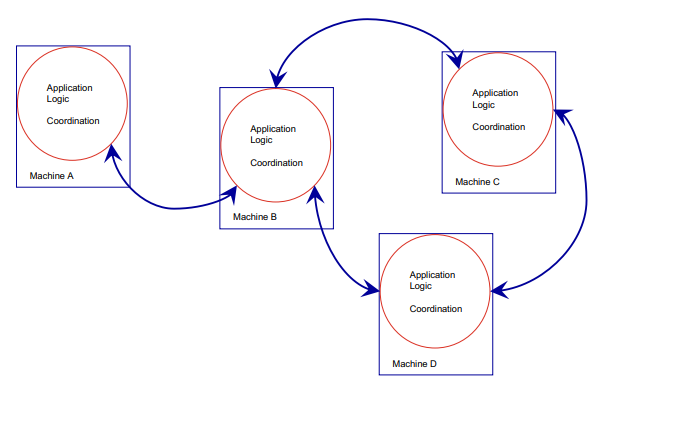
\includegraphics[width = 0.90\textwidth]{Images/1.PNG}
    \end{center}
\end{Definizione}

\begin{Definizione}
    Un sistema distribuito è una \textbf{collezione di elementi autonomi capaci di computazione} che appare ai suoi utenti come \textbf{un singolo sistema coerente}
    \begin{center}
        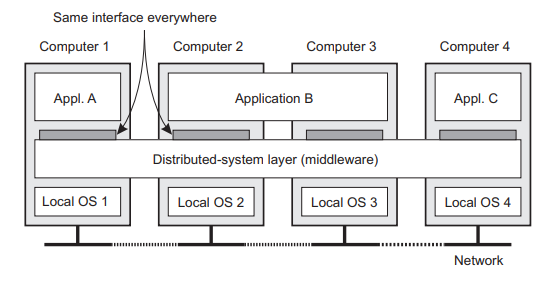
\includegraphics[width = 0.90\textwidth]{Images/2.PNG}
    \end{center}
    Gli elementi capaci di computazione si dicono \textbf{nodi} ed essi possono essere sia componenti \textbf{hardware} che \textbf{software}. \newline
    Gli utenti (o le applicazioni che si interfacciano con il sistema distribuito) percepiscono quindi \textbf{un singolo sistema} piuttosto che una collezione di elementi indipendenti; i nodi quindi \textbf{devono collaborare} per risolvere i compiti richiesti
\end{Definizione}
Quest'ultima definizione introduce però dei concetti e dei problemi fondamentali: \newline
Ogni nodo è \textbf{autonomo} e quindi avrà la \textbf{propria nozione di tempo}: non esiste quindi \textbf{un "orologio" globale}. \newline
Inoltre, se il sistema è una \textbf{collezione di nodi}, come si può gestire \textbf{l'appartenenza di un nodo ad un certo gruppo}? I gruppi possono essere \textbf{aperti}(ogni nodo del sistema \textbf{può partecipare}) oppure \textbf{chiusi}(solo un numero selezionato di nodi possono partecipare). Ciò però introduce un altro problema: \textbf{come facciamo a capire che stiamo interloquendo con un nodo autorizzato}? \newline
In sintesi, una collezione di nodi \textbf{opera sempre nella stessa maniera}, indipendentemente dal dove, quando o come l'interazione dell'utente con il sistema avviene. \newline
Per esempio:
\begin{itemize}
    \item Un utente \textbf{non può capire} dove una certa computazione sta avvenendo
    \item Dove vengono immagazzinati i dati \textbf{dovrebbe essere irrilevante per l'applicazione}
    \item Se certi dati sono stati replicati \textbf{dovrebbe essere completamente nascosto}
\end{itemize}
La parola chiave quindi è \textbf{trasparenza della distribuzione}; tuttavia ciò comporta il problema di \textbf{"fallimenti parziali" del sistema}:
\begin{itemize}
    \item È praticamente inevitabile che, ad un certo istante di tempo, solo \textbf{una parte} del sistema distribuito fallisca
    \item Nascondere i "fallimenti parziali" e la loro risoluzione \textbf{è molto spesso difficile e in generale impossibile da nascondere}
\end{itemize}
Ricapitolando, quindi, elenchiamo \textbf{le caratteristiche che ogni sistema distribuito deve avere}:
\begin{itemize}
    \item \textbf{Gestione della memoria}:
          \begin{itemize}
              \item \textbf{Non c'è memoria condivisa}
              \item La comunicazione avviene attraverso lo \textbf{scambio di messaggi}
              \item Non c'è uno \textbf{stato globale}: ogni componente (nodo, processo, ecc...) conosce \textbf{solo il proprio stato} e può \textbf{sondare lo stato delle altre componenti}
          \end{itemize}
    \item \textbf{Gestione dell'esecuzione}:
          \begin{itemize}
              \item \textbf{Ogni componente è autonoma}, l'esecuzione di un'applicazione avviene quindi in \textbf{maniera concorrente}
              \item Il coordinamento delle attività diventa quindi \textbf{fondamentale} per definire il comportamento \textbf{dell'intera applicazione} e del sistema
          \end{itemize}
    \item \textbf{Gestione del tempo}:
          \begin{itemize}
              \item \textbf{Non c'è un clock globale}
              \item Non c'è possibilità di \textbf{scheduling o di controllo globale}
              \item Il coordinamento avviene \textbf{solo tramite messaggi!}
          \end{itemize}
    \item \textbf{Tipi di fallimenti}:
          \begin{itemize}
              \item \textbf{Fallimenti indipendenti} dei \textbf{singoli nodi}, non ci sono \textbf{fallimenti dell'intero sistema}
          \end{itemize}
\end{itemize}
\subsection{Architetture Software}
Una architettura software \textbf{definisce la struttura del sistema, le interfacce tra i componenti e i pattern di interazione}(i protocolli). I sistemi distribuiti possono essere organizzati in più modi e secondo diversi stili architetturali. In particolare:
\begin{itemize}
    \item \textbf{Modello base: Architettura stratificata (layered)}
          \begin{itemize}
              \item Sistemi operativi
              \item Middleware
          \end{itemize}
    \item \textbf{Architettura a livelli (tier)}
          \begin{itemize}
              \item Applicazioni \textbf{client-server} (2-tier, 3-tier)
          \end{itemize}
    \item \textbf{Architetture basate sugli oggetti}
          \begin{itemize}
              \item Java-Remote Method Invocation (RMI)
          \end{itemize}
    \item \textbf{Architetture centrare sui dati}
          \begin{itemize}
              \item Il \textbf{Web come File System (FS) condiviso}
          \end{itemize}
    \item \textbf{Architetture basate su eventi}
          \begin{itemize}
              \item Applicazioni web dinamiche basate su \textbf{callbacks} (AJAX)
          \end{itemize}
\end{itemize}
\subsubsection{Architetture stratificate (layered)}
Iniziamo dando una definizione di architettura stratificata:
\begin{Definizione}
    Un'architettura \textbf{layered} è un'architettura software che organizza il software in \textbf{layer}. Ogni layer viene costruito basandosi sul \textbf{layer precedente}, il quale è più generale. \newline
    Un layer può quindi essere definito come un (sotto)insieme di \textbf{(sotto)sistemi} con lo stesso \textbf{grado di generalità} \newline
    I layer superiori sono \textbf{più specifici all'applicazione}, mentre i layer inferiori sono \textbf{più generali}
\end{Definizione}
L'idea alla base di un'architettura a strati è semplice: le componenti sono organizzate in \textbf{layer} in modo tale che una componente che si trova nel layer $L_j$ può effettuare una chiamata (\textbf{downcall}) ad una componente nel layer $L_i$ (con $i < j$) e generalmente si aspetta una \textbf{risposta}. Solo in casi \textbf{particolari} una componente effettuerà una chiamata a componenti in layer più alti (\textbf{upcall}). Mostriamo ora \textbf{diversi tipi di architetture a strati}:
\begin{center}
    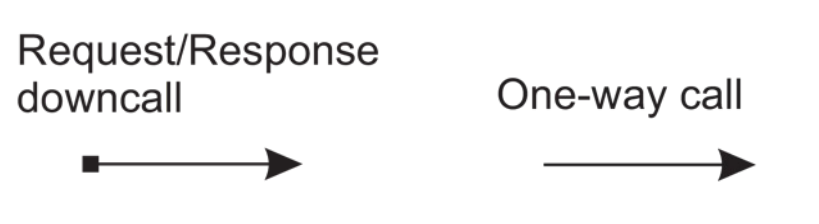
\includegraphics[width = 0.35\textwidth]{Images/3.PNG}
\end{center}
\textbf{Pure layered organization}:
\begin{center}
    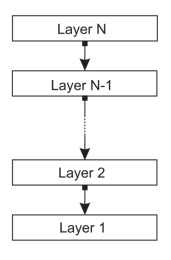
\includegraphics[width = 0.20\textwidth]{Images/4.PNG}
\end{center}
Un esempio di questa architettura è \textbf{lo stack ISO/OSI}:
\begin{center}
    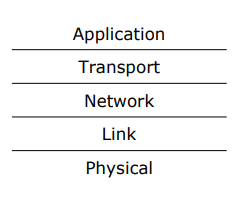
\includegraphics[width = 0.25\textwidth]{Images/5.PNG}
\end{center}
\textbf{Mixed Layer Organization}:
\begin{center}
    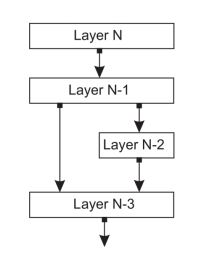
\includegraphics[width = 0.25\textwidth]{Images/6.PNG}
\end{center}
In questo tipo di architettura \textbf{le downcalls possono raggiungere più strati, non sono quello immediatamente successivo}. Un esempio di questa architettura è \textbf{l'organizzazione dei sistemi operativi}:
\begin{center}
    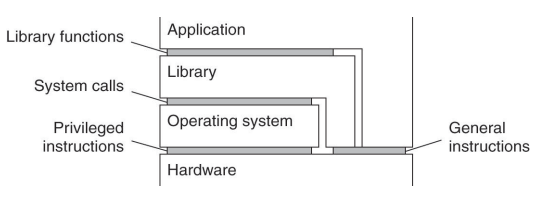
\includegraphics[width = 0.55\textwidth]{Images/7.PNG}
\end{center}
\textbf{Mixed Downcalls and upcalls}:
\begin{center}
    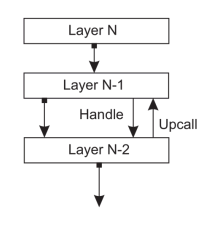
\includegraphics[width = 0.30\textwidth]{Images/8.PNG}
\end{center}
In questa architettura è possibile \textbf{effettuare callbacks e upcalls}. Un esempio di questa architettura sono \textbf{le applicazioni web}:
\begin{center}
    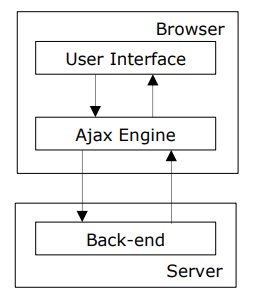
\includegraphics[width = 0.30\textwidth]{Images/9.PNG}
\end{center}
\subsubsection{DOS, NOS e Middleware}
\begin{center}
    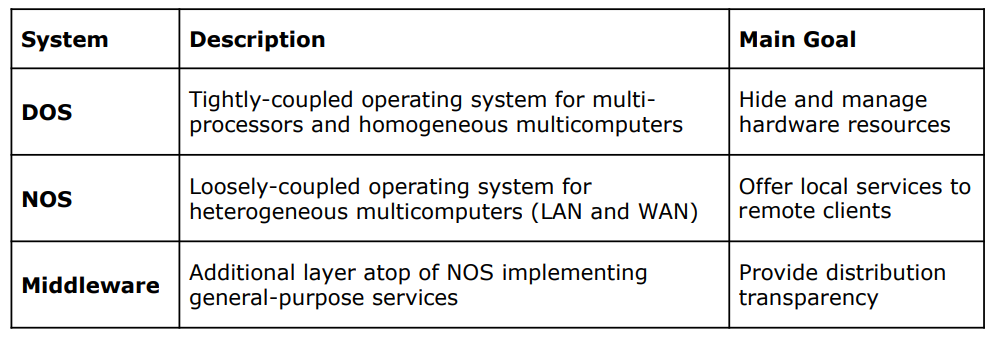
\includegraphics[width = 0.80\textwidth]{Images/10.PNG}
\end{center}
Un \textbf{DOS} (Distributed Operating System) è un sistema operativo \textbf{distribuito} che connette più macchine \textbf{omogenee} attraverso \textbf{un singolo canale di comunicazione}. Il sistema è \textbf{tightly-coupled}, cioè le varie componenti del sistema sono \textbf{interdipendenti}. Ogni nodo del sistema deve essere \textbf{omogeneo rispetto agli altri nodi}.
\begin{center}
    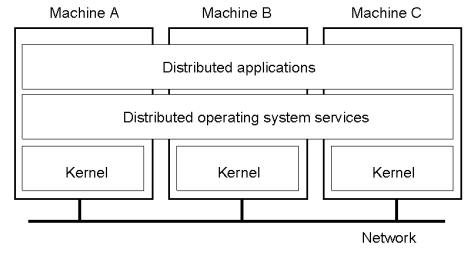
\includegraphics[width = 0.55\textwidth]{Images/11.PNG}
\end{center}
In un DOS, \textbf{l'utente non è consapevole della molteplicità delle macchine che compongono il sistema} (gli è trasparente); l'accesso quindi alle sue risorse sarà, per l'utente, identico all'accesso in \textbf{sistemi formati da un singolo nodo}. Inoltre:
\begin{itemize}
    \item \textbf{Migrazione dei dati}:
          \begin{itemize}
              \item Il trasferimento dati avviene trasferendo \textbf{interi file} o solo le porzioni di essi necessarie ad \textbf{effettuare il compito corrente}
          \end{itemize}
    \item \textbf{Trasferimento della computazione}:
          \begin{itemize}
              \item Piuttosto che trasferire i dati, si preferisce \textbf{trasferire la computazione su tutto il sistema}
          \end{itemize}
    \item \textbf{Migrazione dei processi}: Viene eseguito un intero processo, o parti di esso, \textbf{su differenti nodi}:
          \begin{itemize}
              \item \textbf{Bilanciamento del carico}: Distribuisce i processi \textbf{su tutta la rete} per distribuire equamente il carico
              \item \textbf{Accelerazione della computazione}: I sottoprocessi \textbf{possono essere eseguiti in maniera concorrente su diversi nodi}
              \item \textbf{Preferenze Hardware}: Certe computazione potrebbero richiedere \textbf{hardware specifico}
              \item \textbf{Preferenze Software}: I software richiesti potrebbero \textbf{essere disponibili su un solo nodo}
              \item \textbf{Accesso ai dati}: Si eseguono i processi \textbf{remotamente}, piuttosto che trasferire tutti i dati nel contesto locale
          \end{itemize}
\end{itemize}
Un \textbf{NOS} (Network Operating System) è un sistema operativo \textbf{che mette a disposizione servizi per la comunicazione tra computer all'interno della stessa rete}.
\begin{center}
    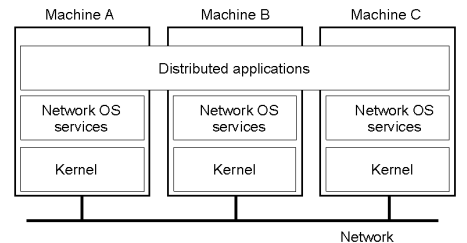
\includegraphics[width = 0.55\textwidth]{Images/12.PNG}
\end{center}
In un NOS, \textbf{gli utenti sono a conoscenza della molteplicità delle macchine che formano il sistema}. Un NOS mette a disposizione \textbf{funzionalità di connettività in maniera esplicita}, tra cui:
\begin{itemize}
    \item Comunicazione \textbf{diretta} tra processi
    \item Esecuzione \textbf{concorrente} (i.e. indipendente) di processi che \textbf{formano un'applicazione distribuita}
    \item Servizi, come \textbf{la migrazione dei processi}, sono \textbf{gestiti dall'applicazione}
\end{itemize}
Accesso a risorse remote presenti sulle varie macchine del sistema è effettuato in maniera esplicita tramite:
\begin{itemize}
    \item Accesso \textbf{remoto} alla macchina appropriata (ssh, telnet)
    \item \textbf{Desktop remoto} (Windows)
    \item \textbf{Trasferimento dati da una macchina all'altra} tramite protocollo FTP (File Transfer Protocol)
\end{itemize}
Per assistere lo sviluppo delle applicazioni distribuite, i sistemi distribuiti sono spesso organizzati in modo da avere \textbf{un layer di software separato} che è \textbf{logicamente "posto sopra"} ai rispetti S.O. dei computer che fanno parte del sistema. Questo layer è chiamato \textbf{middleware}. In un DOS:
\begin{center}
    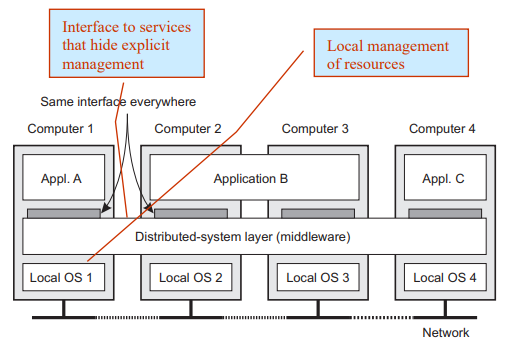
\includegraphics[width = 0.65\textwidth]{Images/13.PNG}
\end{center}
e in un NOS:
\begin{center}
    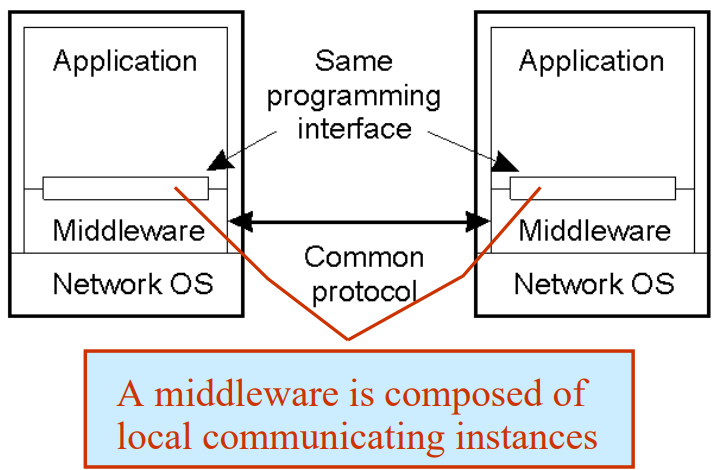
\includegraphics[width = 0.45\textwidth]{Images/14.PNG}
\end{center}
Il middleware si occupa \textbf{implementare dei servizi} e di renderli \textbf{trasparenti alle applicazioni}. I servizi del middleware possono occuparsi di \textbf{diverse questioni} appartenenti a diversi domini, dal più generale al più specifico. Tra di essi vi sono:
\begin{itemize}
    \item \textbf{Nomenclatura}
          \begin{itemize}
              \item Nomi simbolici vengono usati per identificare \textbf{entità del sistema distribuito}
              \item I nomi possono essere usati dai \textbf{registri} per comunicare \textbf{gli indirizzi reali} o possono essere usati \textbf{implicitamente dal middleware}
          \end{itemize}
    \item \textbf{Trasparenza all'accesso}
          \begin{itemize}
              \item Il middleware definisce e offre un \textbf{modello di comunicazione} che nasconde i dettagli \textbf{dello scambio di messaggi}
          \end{itemize}
    \item \textbf{Persistenza}:
          \begin{itemize}
              \item Il middleware definisce un \textbf{servizio automatico di immagazzinamento dati} (su File System o Database)
          \end{itemize}
    \item \textbf{Transazioni distribuite}
          \begin{itemize}
              \item Il middleware definisce un \textbf{modello persistente} per assicurarsi automaticamente della \textbf{consistenza} delle operazioni di lettura/scrittura
          \end{itemize}
    \item \textbf{Sicurezza}
          \begin{itemize}
              \item Il middleware definisce un \textbf{modello} per prevenire accessi non autorizzati (con diversi livelli di permesso) alle risorse, ai servizi e per \textbf{assicurarsi dell'integrità della computazione}
          \end{itemize}
\end{itemize}
Ricapitolando, quindi:
\begin{center}
    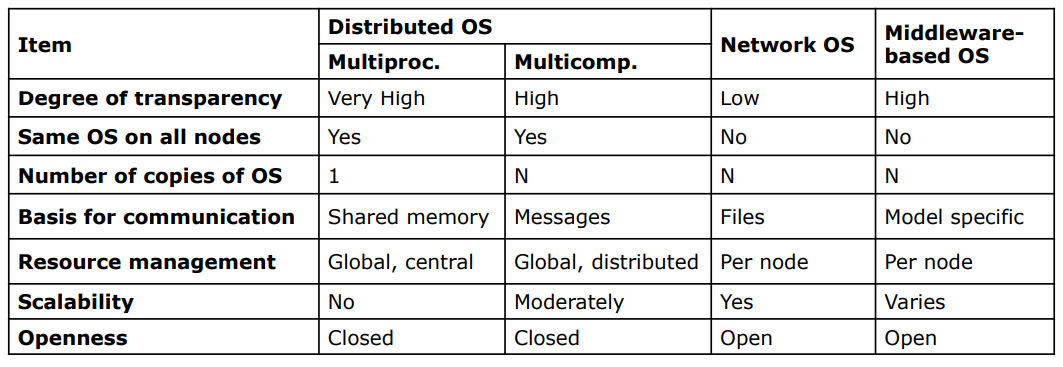
\includegraphics[width = 1\textwidth]{Images/15.PNG}
\end{center}
\subsection{Modello Client-Server}
Il modello \textbf{Client-Server} è un modello di comunicazione che coinvolge un nodo \textbf{richiedente} (Client) e un nodo che \textbf{soddisfa la sua richiesta} (Server). Possiamo quindi vedere il modello base in questo modo:
\begin{center}
    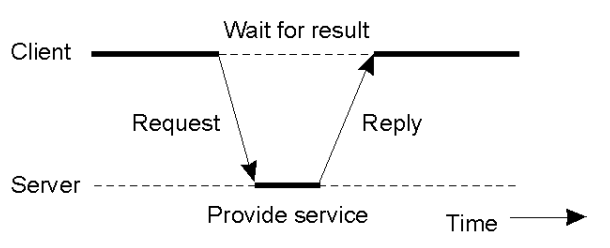
\includegraphics[width = 0.60\textwidth]{Images/16.PNG}
\end{center}
L'architettura di base di questo modello prevede che un \textbf{client} acceda ad un \textbf{server} con una \textbf{richiesta} e che il server \textbf{risponda con un risultato}.
\begin{center}
    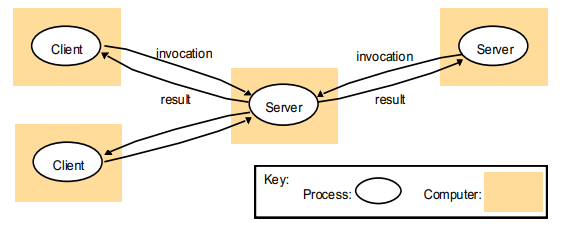
\includegraphics[width = 0.70\textwidth]{Images/17.PNG}
\end{center}
Ciò può avvenire anche tramite \textbf{accesso a server multipli}:
\begin{center}
    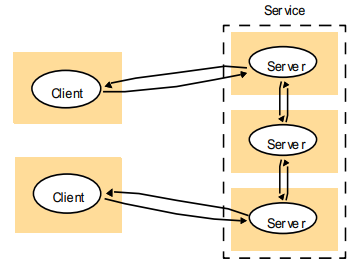
\includegraphics[width = 0.50\textwidth]{Images/18.PNG}
\end{center}
O tramite \textbf{server Proxy}
\begin{center}
    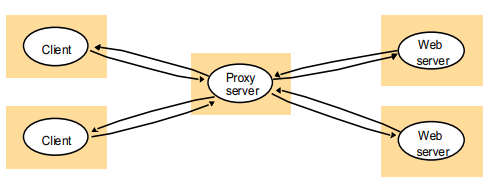
\includegraphics[width = 0.60\textwidth]{Images/19.PNG}
\end{center}
\subsection{Problemi fondamentali di ogni sistema distribuito}
In generale, ogni sistema distribuito deve affrontare \textbf{4 problemi fondamentali}:
\begin{itemize}
    \item \textbf{Identificare la controparte}
          \begin{itemize}
              \item Chi (processo o risorsa) è la mia controparte?
              \item Dobbiamo assegnare dei \textbf{nomi}!
          \end{itemize}
    \item \textbf{Accede alla controparte}
          \begin{itemize}
              \item Come posso raggiungere \textbf{un processo o una risorsa remota}?
              \item Abbiamo bisogno di un \textbf{riferimento}! (\textbf{Access point (AP)})
          \end{itemize}
    \item \textbf{Comunicazione}:
          \begin{itemize}
              \item Come fanno i partecipanti a \textbf{scambiarsi messaggi}?
              \item Dobbiamo concordare su un \textbf{modo di comunicare!} (\textbf{protocollo})
              \item Come fanno i partecipanti a \textbf{capire il significato del messaggio}?
              \item Dobbiamo concordare un sistema di \textbf{sintassi e semantica dei dati} (Ancora una \textbf{questione aperta})
          \end{itemize}
\end{itemize}
\subsubsection{Problema della trasparenza}
Altro problema è quello della \textbf{trasparenza}. La trasparenza di un sistema è la sua capacità di \textbf{nascondere dettagli all'utente, il quale può ignorare cosa effettivamente accade e (sopratutto) non può influenzare il servizio dato}. \newline
La trasparenza può essere implementato su più "livelli":
\begin{itemize}
    \item \textbf{Nomenclatura}
          \begin{itemize}
              \item Nomi simbolici vengono utilizzati per identificare \textbf{parti del sistema distribuito}
          \end{itemize}
    \item \textbf{Trasparenza all'accesso}
          \begin{itemize}
              \item Nasconde \textbf{le differenza nella rappresentazione dei dati} e come si accede alle risorse locali o remote
          \end{itemize}
    \item \textbf{Trasparenza del luogo}
          \begin{itemize}
              \item Nasconde \textbf{dove una certa risorsa risiede nella rete}
          \end{itemize}
    \item \textbf{Trasparenza della riallocazione e della mobilità}
          \begin{itemize}
              \item Nasconde \textbf{che una certa risorsa può essere trasferita in un altro nodo mentre è in uso}
          \end{itemize}
    \item \textbf{Trasparenza della migrazione}
          \begin{itemize}
              \item Nasconde \textbf{che una certa risorsa può essere trasferita}
          \end{itemize}
          \newpage
    \item \textbf{Trasparenza della replicazione}
          \begin{itemize}
              \item Nasconde che una certa \textbf{risorsa può essere stata replicata}
          \end{itemize}
    \item \textbf{Trasparenza della concorrenza}
          \begin{itemize}
              \item Nasconde che una certa risorsa \textbf{può essere condivisa tra più utenti indipendenti} (assicurandosi la consistenza del suo stato)
          \end{itemize}
    \item \textbf{Trasparenza dei fallimenti}
          \begin{itemize}
              \item Nasconde i fallimenti e il recupero di una certa risorsa
          \end{itemize}
    \item \textbf{Trasparenza della persistenza}
          \begin{itemize}
              \item Nasconde che una certa risorsa può \textbf{essere volatile o può venire immagazzinata permanentemente}
          \end{itemize}
\end{itemize}
\subsubsection{Grado di trasparenza}
Ambire alla massima trasparenza in un sistema distribuito potrebbe essere \textbf{impossibile da raggiungere}:
\begin{itemize}
    \item Vi sono \textbf{latenze nella comunicazione che sono impossibili da nascondere}
    \item Nascondere completamente i fallimenti del sistema è \textbf{impossibile sia teoricamente che praticamente}:
          \begin{itemize}
              \item Non si può distinguere un computer lento da uno che sta fallendo
              \item Non si è mai sicuri se un server ha eseguito un compito prima di un crash
          \end{itemize}
    \item Una trasparenza completa \textbf{impatta le performance}, per esempio, richiede del tempo aggiuntivo:
          \begin{itemize}
              \item Tenere le repliche dei dati \textbf{aggiornate con il nodo principale}
              \item Effettuare il flush delle operazioni di scrittura sul disco per permettere la \textbf{tolleranza ai guasti} (fault tolerance)
          \end{itemize}
    \item Esporre la "distribuzione" del sistema potrebbe essere una scelta corretta:
          \begin{itemize}
              \item Permettere all'utente di usare la risorsa \textbf{più vicina}
              \item Gestire utenti in diverse fasce orarie
              \item Esporla quando \textbf{rende all'utente più comprensibile cosa sta accadendo} (es. messaggio di errore di timeout)
          \end{itemize}
\end{itemize}
\newpage
\subsection{Information Hiding e astrazione}
L'Information Hiding è un \textbf{concetto base} dell'ingegneria del software. Essa è la separazione tra \textbf{quale} servizio o componente il sistema offre \textbf{come} il servizio è implementato e "installato" (deployed). \newline
Il \textbf{quale}:
\begin{itemize}
    \item È definito da un "\textbf{Interface Definition Language}" (IDL) atto a definire l'"\textbf{Application Programming Interface}" (API) dei componenti del sistema
    \item Dovrebbe essere \textbf{annotata semanticamente} (cioè dovrebbe descrivere \textbf{le informazioni scambiate} e i \textbf{comportamenti prescritti})
\end{itemize}
Il \textbf{come}:
\begin{itemize}
    \item È implementato con uno \textbf{strumento} (framework, middleware, ecc...) che è \textbf{adatto} per quel problema o all'ambiente in cui il sistema deve operare
    \item Dovrebbe essere implementato con \textbf{algoritmi e tecnologie} efficaci ed efficienti.
\end{itemize}
Le \textbf{interfacce} dovrebbero:
\begin{itemize}
    \item Progettate in base a \textbf{principi comuni} (es. protocolli di comunicazione)
    \item \textbf{complete} (offrire \textbf{tutto il necessario})
    \item \textbf{neutrali} (dovrebbero essere indipendenti dalle altre implementazioni)
    \item \textbf{supportare} \textbf{l'interoperabilità, la portabilità e l'estensibilità}
\end{itemize}
\subsection{Politiche e meccanismi}
Un sistema distribuito dovrebbe essere composto da \textbf{componenti indipendenti}:
\begin{itemize}
    \item \textbf{Indipendenza logica}: Ogni componente \textbf{offre un servizio o svolge una mansione}
    \item \textbf{Composizione}: Ogni componente usa o collabora con altre componenti per \textbf{svolgere o eseguire compiti più complessi}
\end{itemize}
Tutto ciò può essere facilitato tramite una corretta distinzione tra \textbf{politica e meccanismo}:
\begin{itemize}
    \item \textbf{Meccanismo}: Capacità offerte dai componenti (\textbf{come})
    \item \textbf{Politica}: Come le capacità possono essere sfruttate per \textbf{definire un comportamento} (\textbf{quando})
\end{itemize}
Nelle applicazioni reali, \textbf{questa separazione è difficile da ottenere}. Un esempio di meccanismo può essere il \textbf{context switch} per i processi; mentre un esempio di politica può essere \textbf{Round Robin} per lo scheduling dei processi. \newline
C'e però un'osservazione però da compiere: più netta è la separazione tra politica e meccanismo, più ci dobbiamo assicurare che vi siano \textbf{meccanismi adeguati a supporto di queste politiche}. Dobbiamo quindi \textbf{trovare un equilibrio}: Effettuare "\textbf{l'hard-coding}" delle politiche spesso \textbf{semplifica la gestione} e diminuisce le complessità, al costo della \textbf{flessibilità del programma}. Ovviamente, \textbf{non esiste una risposta univoca}.
\subsection{Il concetto di protocollo}
Per formulare le richieste e comprendere i messaggi, i processi in un sistema distribuito devono \textbf{concordare un protocollo}. I protocolli definiscono:
\begin{itemize}
    \item \textbf{Il formato} dei dati
    \item \textbf{L'ordine di invio e di ricezione} dei messaggi tra i dispositivi
    \item \textbf{Il tipo dei dati} scambiati
    \item \textbf{Le azioni} da eseguire quando si riceve un messaggio
\end{itemize}
Le applicazioni su \textbf{TCP/IP}:
\begin{itemize}
    \item Si scambiano \textbf{stream di byte} di lunghezza \textbf{finita} (\textbf{meccanismo})
    \item Gli stream scambiati possono essere \textbf{segmentati in messaggi} (\textbf{politica}) definiti da un \textbf{protocollo condiviso}
\end{itemize}
\begin{center}
    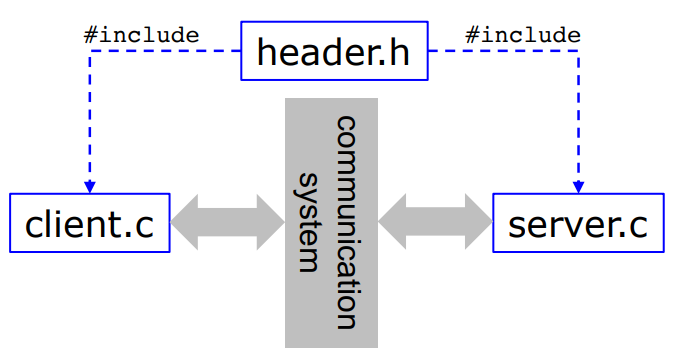
\includegraphics[width = 0.50\textwidth]{Images/20.png}
\end{center}
Nell'esempio sopra, il file \textbf{header.h} definisce il protocollo usato \textbf{sia dal client che dal server}.
\section{Stream-Oriented Communication}
Il reame dei sistemi distribuiti termina alla \textbf{comunicazione interprocesso}; sotto di essa si entra nel dominio delle \textbf{reti di computer}
\begin{center}
    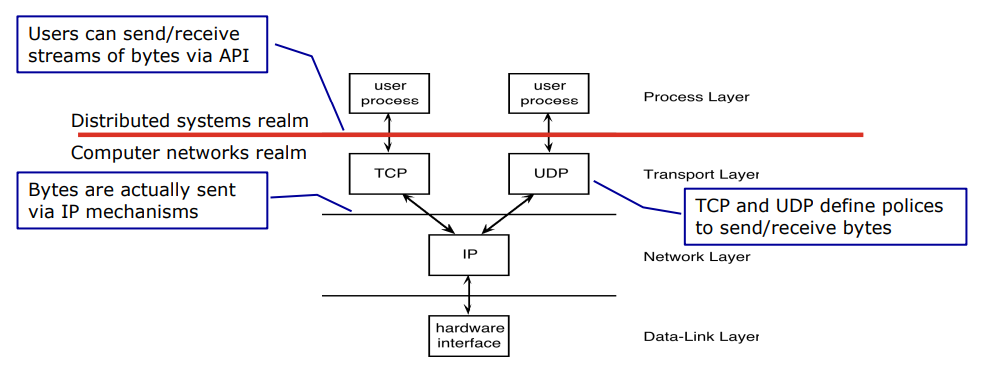
\includegraphics[width = 1\textwidth]{Images/21.png}
\end{center}
Inoltre, i protocolli di rete seguono un' \textbf{architettura a strati}:
\begin{center}
    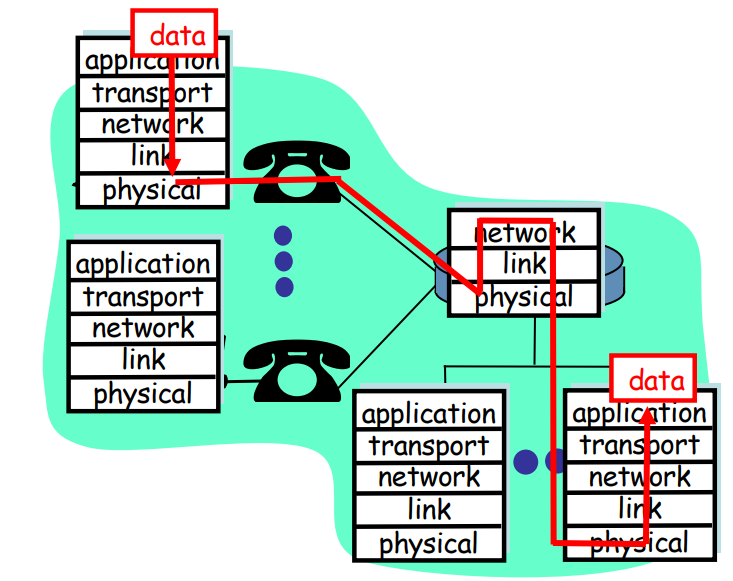
\includegraphics[width = 0.55\textwidth]{Images/22.png}
\end{center}
Diamo inoltre altre definizioni fondamentali:
\begin{itemize}
    \item \textbf{End Systems (Hosts)}
          \begin{itemize}
              \item Ospitano i \textbf{processi che eseguono le applicazioni}
              \item Si trovano ai \textbf{confini della rete}
          \end{itemize}
    \item \textbf{Modello Client-Server}:
          \begin{itemize}
              \item L'host client \textbf{richiede} e \textbf{riceve} un servizio dal \textbf{server}
          \end{itemize}
    \item \textbf{Modello peer-to-peer (P2P)}
          \begin{itemize}
              \item Gli host interagiscono in \textbf{maniera simmetrica}
              \item es. Teleconferenza, \textbf{gnutella}: protocollo di rete e network P2P dedicato alla condivisione di file aperta.
          \end{itemize}
\end{itemize}
\subsection{Processi e programmi}
Un programma \textbf{viene eseguito da un processo} ed esso \textbf{è una serie di istruzioni ordinate eseguibili da una "macchina"}. I processi sono invece \textbf{entità gestite dal Sistema Operativo} ed essi sono formati da:
\begin{itemize}
    \item Un'area di \textbf{memoria RAM} dedicata alla memorizzazione dei dati e all'esecuzione delle operazioni
    \item \textbf{Un registro}, che ricorda la prossima istruzione da eseguire (PC)
    \item \textbf{I canali di comunicazione} del processo
\end{itemize}
In particolare, \textbf{ogni processo comunica attraverso dei canali}:
\begin{itemize}
    \item Un canale gestisce \textbf{flussi di dati in ingresso e in uscita} (in formato \textbf{binario} o testuale)
    \item Schermo e tastiera \textbf{sono esempi di canali}
    \item Dall'esterno, ogni canale è identificato da un \textbf{numero intero} detto \textbf{porta}
\end{itemize}
Le \textbf{socket} sono particolari tipi di canali per la comunicazione tra \textbf{processi} che \textbf{non condividono memoria}. Per potersi connettere o inviare dati ad un processo A, il processo B deve \textbf{conoscere la macchina} (host) che esegue A e la \textbf{porta a cui A è connesso}. Essa può essere una porta arbitraria o una \textbf{porta nota per convenzione} (well-known port).
\subsection{Servizi di trasporto internet: TCP e UDP}
Facciamo un riassunto dei servizi di due protocolli di trasporto: \textbf{TCP} e \textbf{UDP}. \newline
Iniziamo da \textbf{TCP} (Transmission Control Protocol):
\begin{itemize}
    \item \textbf{Orientato alla connessione}: Il client invia al server \textbf{una richiesta di connessione}
    \item \textbf{Trasporto affidabile}(reliable transfer): Il trasporto e la ricezione tra mittente e destinatario è \textbf{garantito}.
    \item \textbf{Controllo di flusso}(flow control): Il mittente \textbf{rallenta per non sommergere il ricevente}
    \item \textbf{Controllo della congestione}(congestion control): Il mittente \textbf{rallenta quando la rete è sovraccarica}
    \item \textbf{Non offre garanzie di banda o latenza minima}
    \item Protocollo \textbf{affidabile}
\end{itemize}
Passando invece ad \textbf{UDP} (User Datagram Protocol):
\begin{itemize}
    \item Trasporto \textbf{non affidabile} tra processi mittente e ricevente
    \item Non offre \textbf{connessione, affidabilità, controllo di flusso o di congestione e garanzie di banda o di ritardo}
    \item Perché esiste UDP? A volte può essere \textbf{conveniente}: per esempio nelle applicazioni che \textbf{tollerano una perdita parziale di dati} come le applicazioni di streaming video o audio.
    \item Protocollo \textbf{Best-Effort}
\end{itemize}
Entrambi i protocolli quindi offrono dei servizi, i quali sono soggetti a \textbf{politiche diverse}. \newline
Il \textbf{servizio di UDP}:
\begin{itemize}
    \item \textbf{Scompone il flusso di byte in segmenti}
    \item Li invia uno per volta ai servizi di rete
\end{itemize}
Mentre il \textbf{servizio di TCP}:
\begin{itemize}
    \item Scompone ed invia \textbf{come UDP}
    \item Ogni segmento viene \textbf{numerato} per garantire:
          \begin{itemize}
              \item Il \textbf{riordinamento} dei segmenti arrivati
              \item Il \textbf{controllo delle duplicazioni} (scarto i segmenti con numero di sequenza uguale)
              \item Il \textbf{controllo delle perdite} (rinvio dei segmenti mancanti)
          \end{itemize}
\end{itemize}
Tuttavia, per progettare sistemi distribuiti \textbf{non è necessario conoscere il funzionamento dei processi} (information hiding), ma ciò che importa è conoscere come \textbf{avviene lo scambio di dati} (byte) tra processi.
\subsection{Socket: funzionamento di base}
Il protocollo TCP:
\begin{itemize}
    \item Utilizza variabili per realizzare il \textbf{trasferimento bidirezionale} di flussi di bytes ("pipe") tra processi
    \item Prevede ruoli client/server per la \textbf{connessione} ma non per la \textbf{comunicazione}
    \item Utilizza i servizi dello \textbf{strato di rete} (IP) per l'invio dei flussi di bytes
\end{itemize}
Per utilizzare il protocollo facciamo uso di un'API, che \textbf{definisce l'interfaccia tra l'applicazione e lo strato di trasporto}. Una \textbf{Socket} è un canale di comunicazione tra due processi; essa si può definire \textbf{sia per TCP che per UDP}. In generale, due processi comunicano \textbf{inviando/leggendo} dati \textbf{in/da Socket}.
\begin{center}
    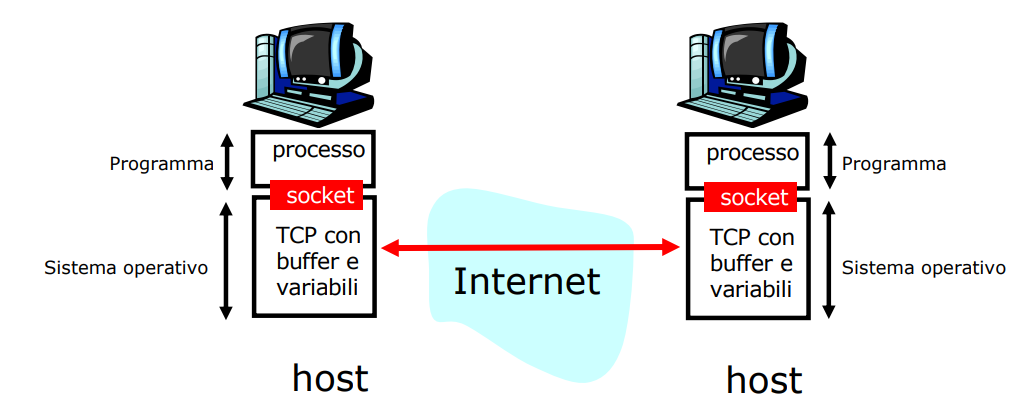
\includegraphics[width = 0.75\textwidth]{Images/23.png}
\end{center}
\subsection{Aspetti critici}
Vi sono diversi aspetti critici da risolvere quando si progetta un sistema distribuito:
\begin{itemize}
    \item \textbf{Gestione del ciclo di vita Client-Server}
          \begin{itemize}
              \item Attivazione/terminazione del \textbf{client e del server}: può essere manuale oppure \textbf{gestita da un middleware}
          \end{itemize}
          \newpage
    \item \textbf{Identificazione e accesso al server}
          \begin{itemize}
              \item Informazioni che il \textbf{client deve conoscere} per accedere al server
          \end{itemize}
    \item \textbf{Comunicazione tra client e server}
          \begin{itemize}
              \item Le primitive disponibili e le \textbf{modalità} di comunicazione (es. TCP/IP: Stream di dati inviati con send/receive)
          \end{itemize}
    \item \textbf{Ripartizione dei compiti tra client e server}
          \begin{itemize}
              \item Dipende dall'applicazione
              \item Influenza \textbf{le prestazioni} in relazione al carico
          \end{itemize}
\end{itemize}
\subsubsection{Identificazione del server}
Come fa il client a conoscere l'indirizzo del server? Ci sono varie alternative:
\begin{itemize}
    \item Inserire nel codice del client l'indirizzo del server espresso come \textbf{costante}
    \item \textbf{Chiedere all'utente l'indirizzo}
    \item \textbf{Utilizzare un name server o una repository} da cui il client può estrarre le informazioni necessarie (DNS per esempio)
    \item \textbf{Adottare un protocollo} per l'individuazione del server (es. \textbf{Broadcast DHCP})
\end{itemize}
\subsubsection{Risoluzione degli aspetti critici in TCP/IP}
Come vengono risolti gli aspetti critici in TCP/IP?
\begin{itemize}
    \item \textbf{Identificare la controparte}(naming): Identificazione \textbf{a basso livello}: nome degli hosts e \textbf{protocolli}
    \item \textbf{Accesso alla controparte}(Access point): Uso dell'\textbf{indirizzo IP}(host:port) per accedere al processo.
    \item \textbf{Comunicazione}:
          \begin{itemize}
              \item \textbf{Protocollo}: Stream di byte
              \item \textbf{Sintassi e semantica}: Protocolli applicativi con \textbf{sintassi e semantica predefiniti}
          \end{itemize}
\end{itemize}
Qual è il livello di trasparenza di queste risoluzioni? \textbf{Molto basso} poiché il programmatore/utente deve \textbf{conoscere gli indirizzi IP degli agenti} e \textbf{deve effettuare il parsing dei byte} per ottenere il contenuto del messaggio.
\newpage
\subsection{Comunicazione via Socket}
La comunicazione TCP/IP avviene tramite \textbf{flussi di bytes} (byte stream) dopo una \textbf{connessione esplicita}, tramite normali \textbf{system call} read/write.
Queste due system call:
\begin{itemize}
    \item \textbf{Sono sospensive}, cioè bloccano il processo finché lo scheduler del sistema operativo \textbf{non lo riporta nello stato di esecuzione}
    \item \textbf{Utilizzano un buffer} per garantire la \textbf{flessibilità}, per esempio il buffer può essere lungo $N$ caratteri, ma ciò che è presente sul canale può essere uno stream lungo $k < N$ caratteri.
\end{itemize}
Le diverse fasi della comunicazione sono riassumibili nella seguente immagine:
\begin{center}
    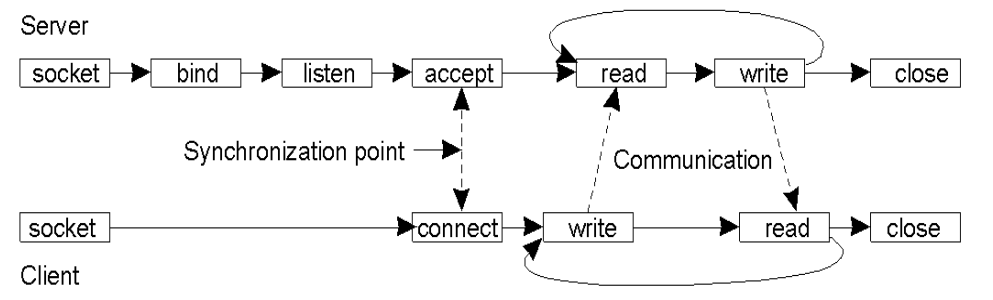
\includegraphics[width = 0.85\textwidth]{Images/24.png}
\end{center}
La fase fino alla chiamata \textbf{accept} è detta di \textbf{CONNESSIONE} mentre la fase successiva è detta di \textbf{CONVERSAZIONE}. Ricordiamo inoltre che le Socket \textbf{SONO OGGETTI CONCETTUALI}, cioè mi permettono di definire un \textbf{canale sicuro di comunicazione}, ma non hanno una controparte fisica. I canali di comunicazione sono \textbf{TUTTI UGUALI}: per questo corso seguiamo il \textbf{MODELLO UNIX}, cioè i canali di comunicazione sono dei \textbf{FILE}. Infine, notiamo che \textbf{le capacità di lettura e scrittura di un sistema dipendono anche dall'infrastruttura di rete sottostante}, tuttavia le applicazioni dovrebbero esserne \textbf{indipendenti}. \newline
IL protocollo delle Socket è \textbf{codificato a basso livello}: il flusso di byte \textbf{NON È UN MESSAGGIO}, i messaggi sono costruiti dalle applicazioni. \newline
Diverse chiamate sono offerte per accedere a TCP e UDP, riportiamo le più importanti qui sotto:
\begin{center}
    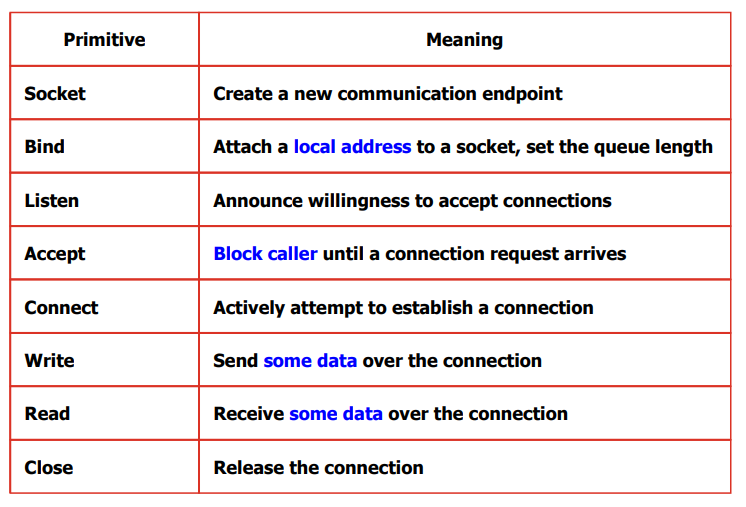
\includegraphics[width = 0.65\textwidth]{Images/25.png}
\end{center}
\subsection{Processi e Socket}
Il server crea una \textbf{Socket collegata ad una well-known port} (che identifica il servizio fornito) dedicata a \textbf{ricevere richieste di connessione}. Con la chiamata di sistema \textbf{accept()}, il server crea \textbf{una nuova Socket}, cioè \textbf{un nuovo canale}, dedicato alla comunicazione del client. \newline
Vediamo la progressione della comunicazione:
\newline
\textbf{1: Il server crea una Socket per accettare le connessioni} e gli assegna un indirizzo IP tramite \textbf{bind()}
\begin{center}
    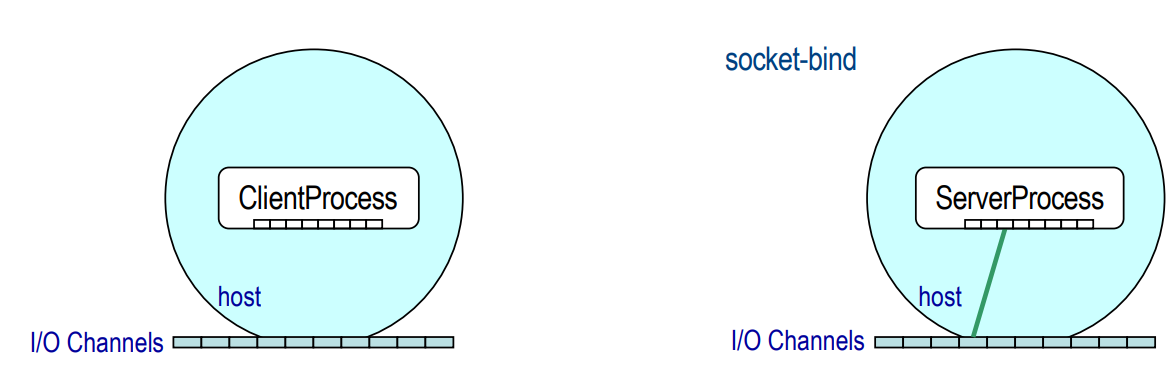
\includegraphics[width = 0.75\textwidth]{Images/26.png}
\end{center}
\textbf{2: Il client crea una Socket per comunicare con il server}
\begin{center}
    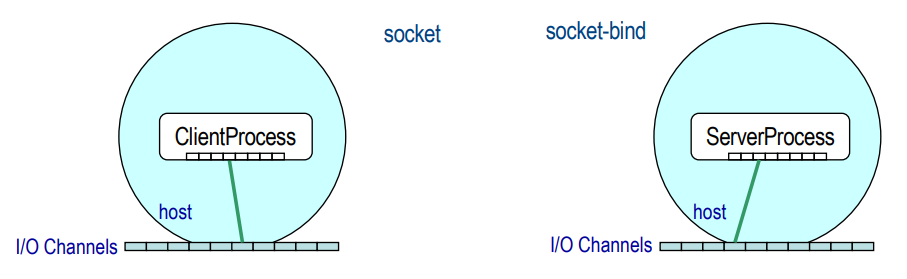
\includegraphics[width = 0.75\textwidth]{Images/27.PNG}
\end{center}
\textbf{3: Il client si fa una richiesta di connessione al server}
\begin{center}
    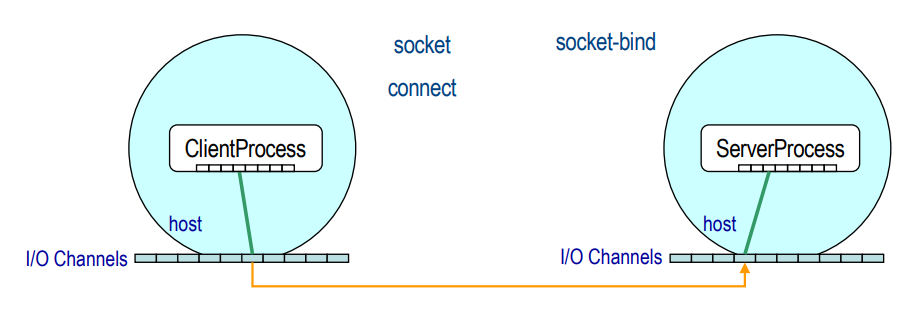
\includegraphics[width = 0.75\textwidth]{Images/28.PNG}
\end{center}
\textbf{4: Il server accetta la connessione} e assegna una nuovo canale al Client. Ciò avviene per due ragioni: \textbf{lasciare la socket iniziale libera per accettare nuove connessioni} e \textbf{dedicare un canale apposito alla comunicazione interprocesso} adibito ai messaggi applicativi.
\begin{center}
    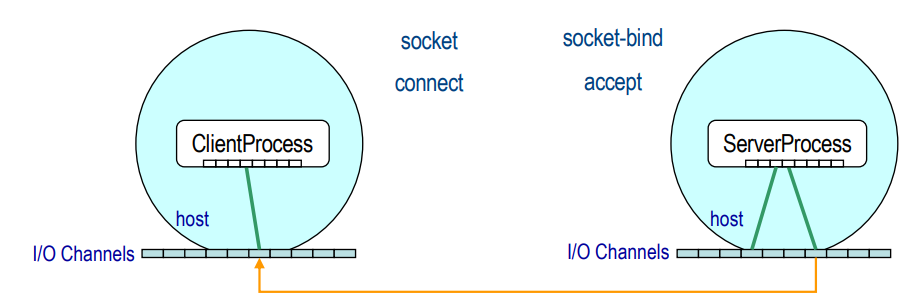
\includegraphics[width = 0.75\textwidth]{Images/29.PNG}
\end{center}
\textbf{5: La connessione viene stabilita} e vengono iniziate le operazioni di lettura/scrittura
\begin{center}
    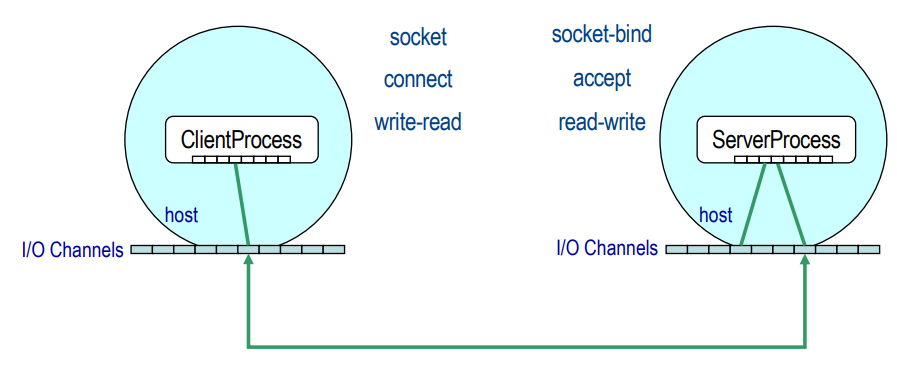
\includegraphics[width = 0.75\textwidth]{Images/30.PNG}
\end{center}
Ricordiamo che le Socket \textbf{trasportano flussi di bytes}, quindi:
\begin{itemize}
    \item Non esiste il concetto di \textbf{messaggio} (il flusso è continuo e senza fine)
    \item La lettura/scrittura avviene \textbf{per un numero arbitrario di byte}
\end{itemize}
Un prototipo della funzione read potrebbe quindi essere:
\begin{para}
    \begin{lstlisting}
byteletti read(socket, buffer, dimBuffer);
\end{lstlisting}
\end{para}
Con:
\begin{itemize}
    \item \textbf{byteletti}: byte effettivamente letti
    \item \textbf{socket}: il canale da cui leggere
    \item \textbf{buffer}: lo spazio di memoria dove trasferire i byte
    \item \textbf{dimBuffer}: dimensione del buffer = n° max di byte che si possono leggere
\end{itemize}
In un applicazione distribuita quindi si dovranno prevedere \textbf{dei veri e propri cicli di lettura} che termineranno in base alla \textbf{dimensione dei messaggi} come stabilito dal \textbf{protocollo applicativo in uso}
\subsection{Socket in Java}
Java definisce alcune \textbf{classi} che costituiscono delle interfacce alle \textbf{system call} illustrate in precedenza. Le due principali sono:
\begin{itemize}
    \item \textbf{java.net.Socket}
    \item \textbf{java.net.ServerSocket}
\end{itemize}
Queste classi accorpano \textbf{funzionalità} e \textbf{mascherano} alcuni dettagli con il vantaggio di \textbf{semplificarne l'uso da parte del programmatore}. Tuttavia, come ogni framework, è necessario saperne \textbf{il funzionamento} e il \textbf{modello} per usarlo in maniera del tutto efficace.
\subsubsection{java.net.Socket}
Questa classe implementa \textbf{socket client} (anche semplicemente chiamate socket). Una socket è un \textbf{endpoint} per la comunicazione tra due macchine. Il lavoro della Socket è in verità effettuato da un'istanza della classe \textbf{SocketImpl}. Un'applicazione, modificando il modo in cui vengono costruite le implementazione delle Socket, può configurarsi per creare Socket \textbf{appropriate al firewall locale}.
\begin{center}
    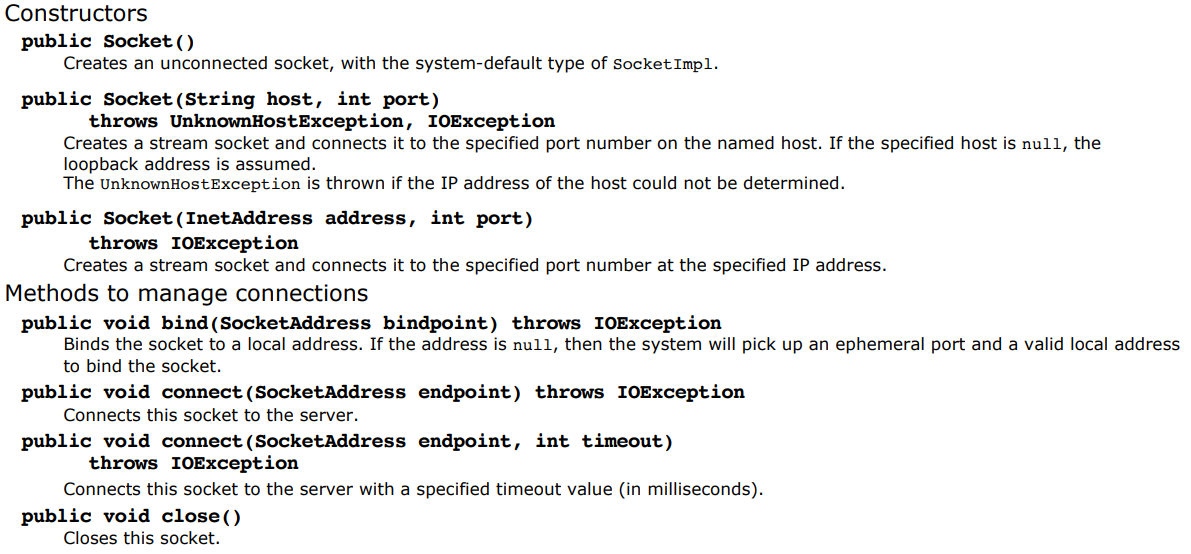
\includegraphics[width = 1.15\textwidth]{Images/31.PNG}
\end{center}
\begin{center}
    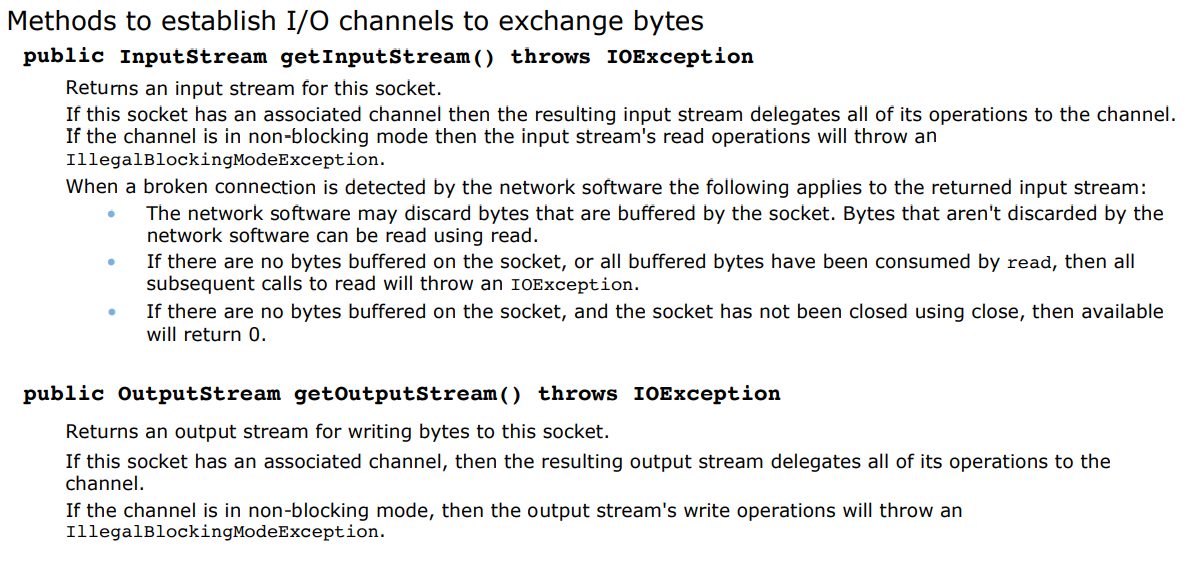
\includegraphics[width = 1.15\textwidth]{Images/32.PNG}
\end{center}
\subsubsection{java.net.ServerSocket}
Questa classe implementa \textbf{server Sockets}. Una server socket \textbf{aspetta che una richiesta giunga dalla rete}, effettua qualche operazione quando riceve la richiesta e \textbf{possibilmente ritorna qualcosa al richiedente}. Il lavoro della ServerSocket è in verità effettuato da un'istanza della classe \textbf{SocketImpl}. Un'applicazione, modificando il modo in cui vengono costruite le implementazione delle Socket, può configurarsi per creare Socket \textbf{appropriate al firewall locale}.
\begin{center}
    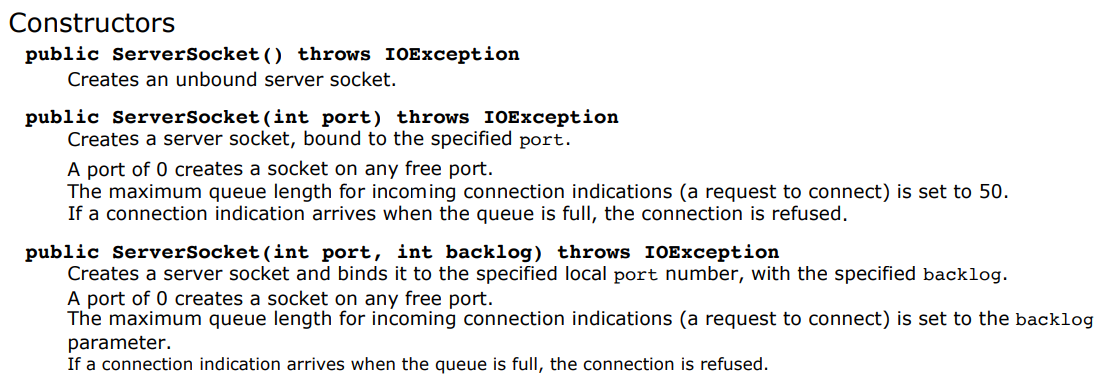
\includegraphics[width = 1.15\textwidth]{Images/33.PNG}
\end{center}
\begin{center}
    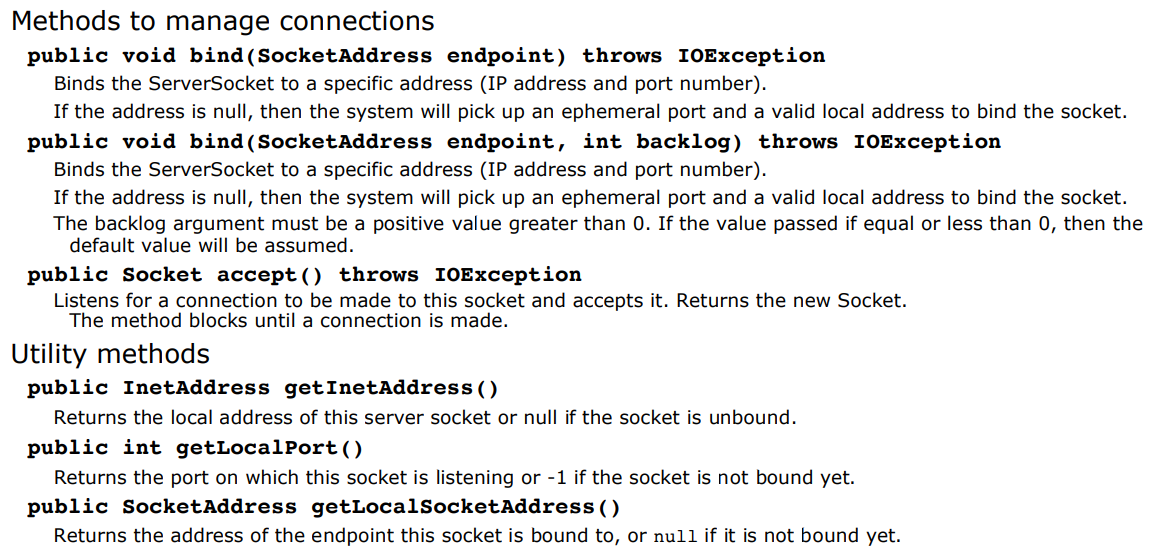
\includegraphics[width = 1.15\textwidth]{Images/34.PNG}
\end{center}
\subsection{Problematiche legate alla latenza}
In un architettura client-server, potremmo avere un \textbf{server che invia un certo numero di dati ogni k istanti di tempo} (LazyServer). Per leggere quindi tutte le informazioni mandate dal server, dobbiamo assicurarci che il client possegga \textbf{un ciclo di lettura continuo}. I dati dalle Socket infatti \textbf{dovrebbero sempre essere letti con un loop!}
\subsection{Progettare un'applicazione con le Socket}
Prendiamo in analisi i due attori del modello client-server:
\begin{itemize}
    \item \textbf{Client}: L'architettura è \textbf{concettualmente più semplice di quella del server}
          \begin{itemize}
              \item È spesso un'applicazione \textbf{convenzionale} che una Socket al posto di un altro canale di I/O
              \item Ha effetti \textbf{solo sugli utenti del client}: non ci sono particolari problemi di sicurezza
          \end{itemize}
    \item \textbf{Server}: L'architettura generale prevede che:
          \begin{itemize}
              \item Venga creata una Socket \textbf{con una porta nota} per accettare le richieste di connessione
              \item Entri un ciclo infinito dove alternare:
                    \begin{enumerate}
                        \item \textbf{attesa/accettazione} di una richiesta di connessione da un client
                        \item \textbf{ciclo di lettura-esecuzione}, invio della riposta al termine della conversazione (stabilita spesso dal client)
                        \item \textbf{chiusura della connessione}
                    \end{enumerate}
          \end{itemize}
\end{itemize}
Vi sono però delle \textbf{problematiche connesse a questo modello}:
\begin{itemize}
    \item L'affidabilità del server è \textbf{strettamente collegata all'affidabilità della comunicazione tra esso e il client}
    \item La modalità connection-oriented determina:
          \begin{itemize}
              \item \textbf{L'impossibilità di rilevare interruzioni sulla connessione} (il client monitora il server)
              \item \textbf{la necessità di una socket per ogni comunicazione}
              \item \textbf{problemi di sicurezza per la condivisione dei dati} e il \textbf{controllo del client}
          \end{itemize}
\end{itemize}
\section{Architetture Server}
I server possono essere di diversi tipi:
\begin{itemize}
    \item \textbf{Iterativi}: soddisfano una richiesta alla volta
    \item \textbf{Concorrenti a processo singolo}: simulano la presenza di un server dedicato
    \item \textbf{Concorrenti multi-processo}: creano server dedicati
    \item \textbf{Concorrenti multi-thread}: creano thread dedicati
\end{itemize}
\subsection{Progettazione di un server iterativo}
Al momento della connessione del client, il server \textbf{crea un socket} temporanea per stabile la connessione diretta. Le eventuali nuove richieste verranno \textbf{accodate alla porta principale} per poi essere soddisfatte più tardi. Il vantaggio di questa architettura è \textbf{la facilità della progettazione}, tuttavia essa è capace solo di \textbf{rispondere ad un solo client alla volta} e un client \textbf{può impedire l'evoluzione degli altri client}. Inoltre, l'architettura \textbf{non è scalabile}.
\begin{center}
    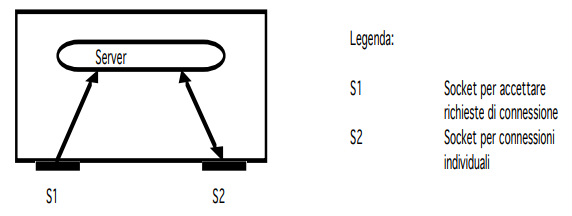
\includegraphics[width = 0.80\textwidth]{Images/35.PNG}
\end{center}
La soluzione ai problemi di quest'architettura sono \textbf{i server concorrenti}.
\subsection{Progettazione di un server concorrente}
Un server concorrente può \textbf{gestire più client in maniera contemporanea}. La sua realizzazione può essere:
\begin{itemize}
    \item \textbf{Simulata con un solo processo}
          \begin{itemize}
              \item Tramite la funzione \textbf{select} (C), in Java tramite la classe, \textbf{Selector}, che conosce \textbf{i canali pronti all'uso}
                    \begin{center}
                        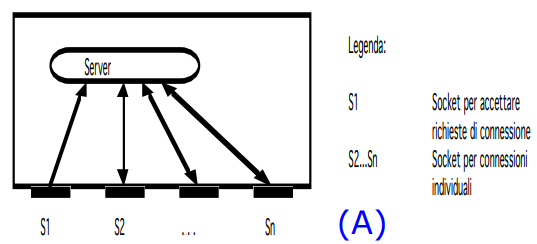
\includegraphics[width = 0.80\textwidth]{Images/36.PNG}
                    \end{center}
                    \newpage
              \item Tramite l'uso di \textbf{Thread}:
                    \begin{center}
                        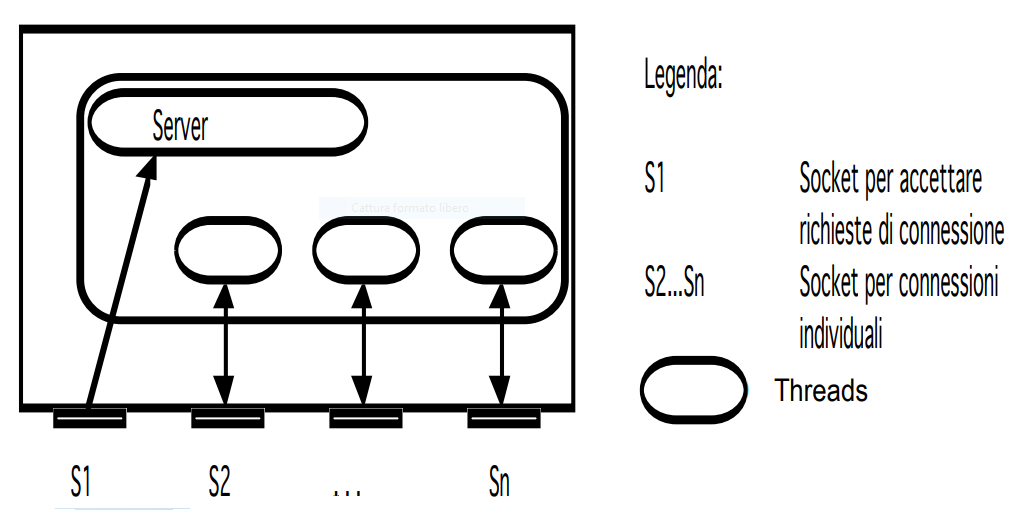
\includegraphics[width = 0.80\textwidth]{Images/37.PNG}
                    \end{center}
          \end{itemize}
    \item \textbf{Reale tramite la creazione di nuovi processi "slave"}
          \begin{itemize}
              \item \textbf{Uso della funzione fork}(C)
                    \begin{center}
                        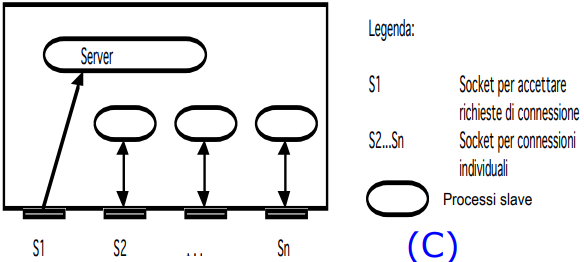
\includegraphics[width = 0.80\textwidth]{Images/38.PNG}
                    \end{center}
          \end{itemize}
\end{itemize}
\subsection{I/O non bloccante}
Le operazioni di lettura e scrittura \textbf{comportano l'uso di system call bloccanti}; cioè che portano \textbf{all'attesa della conclusione dell'operazione richiesta} prima di restituire il controllo al chiamante (il processo può uscire dallo stato di execute). Inoltre, ogni system call deve \textbf{effettuare un context switch del processo chiamante}, che potrebbe quindi portarlo fuori dallo di esecuzione (dipende dalla politica di scheduling). Per leggere in modo non bloccante si deve \textbf{sapere a priori se il canale è pronto o meno}; la system call \textbf{select()} ha questo compito. Il codice del server diventa quindi simile a:
\begin{enumerate}
    \item Dico al sistema \textbf{quali canali voglio usare in maniera non bloccante}
    \item Chiamo la select(), che controlla quali canali sono \textbf{pronti}
    \item Sui canali pronti eseguo l'operazione \textbf{read()}/\textbf{write()} desiderata
    \item Ciclo tornando al punto 1.
\end{enumerate}
\subsubsection{System Call select}
La system call \textbf{select()} permette di gestire in modo non bloccante i diversi canali di I/O:
\begin{center}
    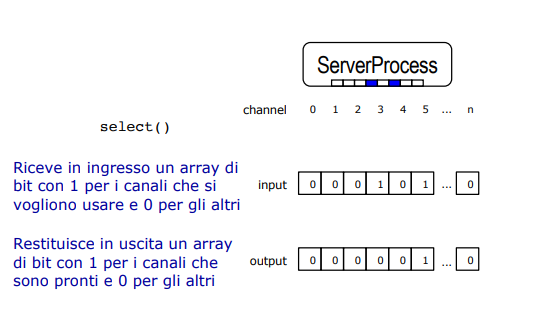
\includegraphics[width = 0.80\textwidth]{Images/39.PNG}
\end{center}
Un server concorrente quindi \textbf{realizza il seguente ciclo}:
\begin{center}
    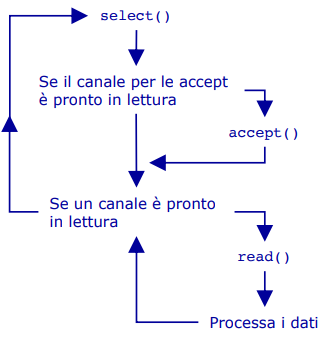
\includegraphics[width = 0.40\textwidth]{Images/40.PNG}
\end{center}
\subsection{I/O non bloccante in Java}
Dalla versione \textbf{1.4 di Java} sono stati introdotti i \textbf{channel}, che possono operare in \textbf{maniera bloccante o non bloccante}.
\begin{itemize}
    \item Un canale non bloccante \textbf{mette il chiamante nello stato di sleep}
    \item L'operazione richiesta \textbf{o viene effettuata} oppure \textbf{viene ritornato che nulla è stato fatto}
\end{itemize}
Tuttavia \textbf{solo i canali Socket possono essere usati in maniera bloccante o non bloccante}; inoltre, essi possono essere usati per \textbf{interagire con i canali di rete}. Sono implementati in Java dalle classi \textbf{ServerSocketChannel}, \textbf{SocketChannel} e \textbf{DatagramChannel}. I canali socket impostati in maniera non bloccante possono essere utilizzati con i \textbf{selector}:
\begin{itemize}
    \item Possono essere gestite in modo più efficiente dalle socket \textbf{definite in java.net}
    \item Permettono gestire più canali in multiplex
\end{itemize}
\subsubsection{java.nio.channels}
Un \textbf{channel} è rappresenta una connessione aperta ad un'entità come una componente hardware, un file, una socket di rete o ad una componente di un programma capace di effettuare diverse operazioni di I/O. L'interfaccia channel \textbf{è estesa da diverse altre interfacce}. In particolare:
\begin{itemize}
    \item \textbf{ServerSocketChannel}: Un canale \textbf{selezionabile} per socket d'ascolto \textbf{stream-oriented}
    \item \textbf{SocketChannel}: Un canale \textbf{selezionabile} per socket di connessione \textbf{stream-oriented}
    \item \textbf{DatagramChannel}:  Un canale \textbf{selezionabile} per socket datagram-oriented
\end{itemize}
\subsubsection{Selector in Java}
Un \textbf{Selector} permette di gestire più \textbf{SelectableChannels} in Java tramite l'uso di una \textbf{select()}. Un selettore può essere creato invocando il metodo statico \textbf{open()}:
\begin{center}
    \textbf{Selector selector = Selector.open();}
\end{center}
I canali da monitorare con la select devono:
\begin{enumerate}
    \item Essere impostati in \textbf{modalità non bloccante}
    \item Registrati tramite il metodo \textbf{register(Selector, MODE)}
\end{enumerate}

\begin{center}
    \textbf{channel.configureBlocking(false);}\newline
    \textbf{SelectionKey key = channel.register(selector, SelectionKey.OP\textunderscore READ);}
\end{center}
Ogni canale può essere impostato per monitorare \textbf{quattro tipi diversi di eventi} definiti attraverso delle costanti della classe \textbf{SelectionKey}
\begin{enumerate}
    \item \textbf{OP\textunderscore CONNECT}: Quando un client cerca di connettersi
    \item \textbf{OP\textunderscore ACCEPT}: Quando un server accetta la richiesta di un client
    \item \textbf{OP\textunderscore READ}: Quando il \textbf{server} è pronto a leggere dal canale
    \item \textbf{OP\textunderscore WRITE}: Quando il \textbf{server} è pronto a scrivere dal canale
\end{enumerate}
Gli oggetti della classe \textbf{SelectionKey} identificano i \textbf{canali} su cui fare le operazioni desiderate. \newline
Proponiamo un esempio in pseudocodice:
\begin{center}
    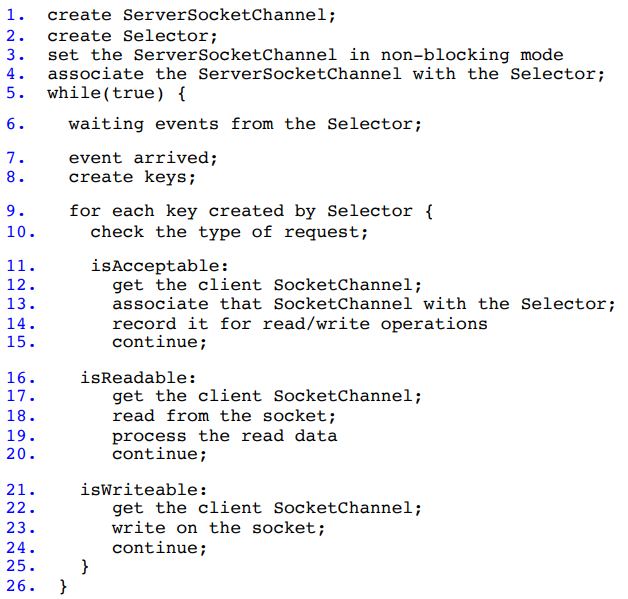
\includegraphics[width = 0.80\textwidth]{Images/41.PNG}
\end{center}
\subsection{Progettare un server multiprocesso}
Un server concorrente (in C) che crea nuovi processi slave lo fa attraverso la chiamata di sistema \textbf{fork()}. La fork() crea un processo clone che:
\begin{itemize}
    \item \textbf{Eredita i canali di comunicazione}
    \item Esegue \textbf{lo stesso codice}
\end{itemize}
Il codice deve quindi prevedere che:
\begin{itemize}
    \item Il padre \textbf{chiuda la socket per la conversazione con il client}
    \item Il figlio \textbf{chiuda la socket per l'accettazione di nuove connessioni}
\end{itemize}
La struttura di questo tipo di server è \textbf{analoga alla forma iterativa}, poiché \textbf{ogni nuovo sottoprocesso gestisce solo un client}.
\begin{center}
    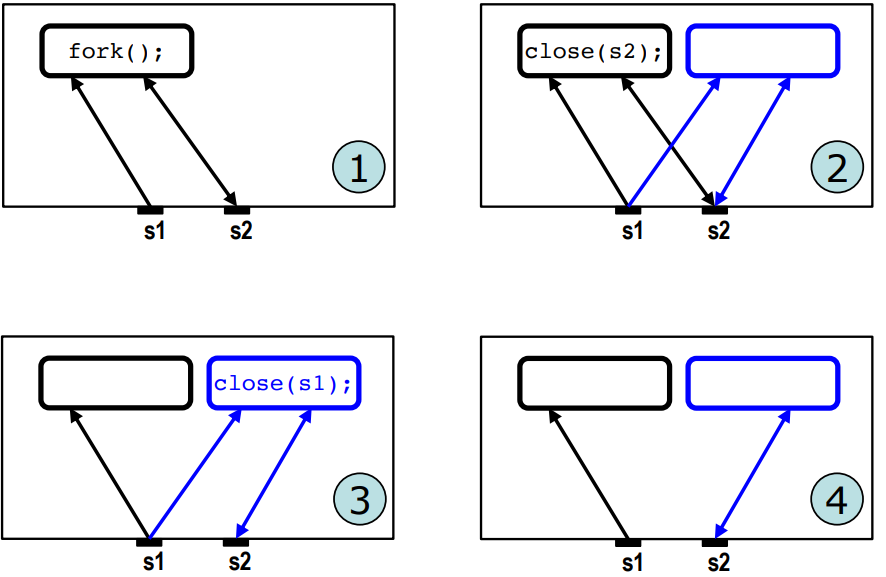
\includegraphics[width = 0.70\textwidth]{Images/42.PNG}
\end{center}
\subsection{Condivisione del canale}
La lettura/scrittura sulla \textbf{stessa Socket} da parte di più processi comporta \textbf{un problema di concorrenza}: viene fatto accesso ad una \textbf{risorsa condivisa}.
\begin{center}
    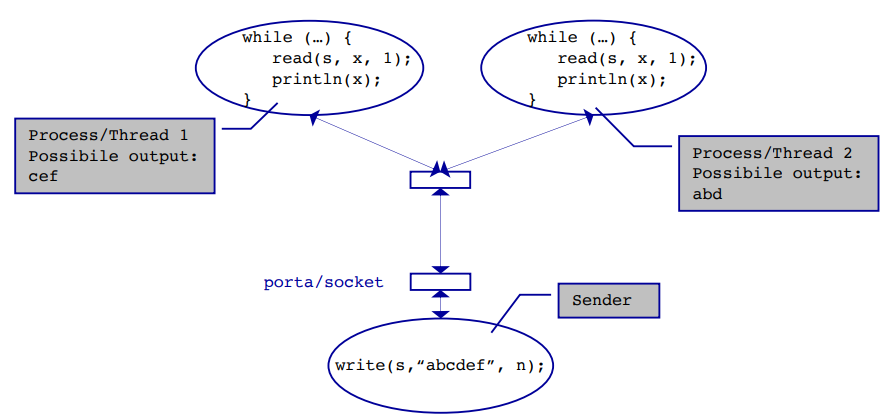
\includegraphics[width = 0.90\textwidth]{Images/43.PNG}
\end{center}
\subsection{Creare un processo clone in Java}
Java non supporta la creazione di nuovi processi con delle \textbf{fork() UNIX-Like}, ma i processi possono essere clonati tramite \textbf{public final class ProcessBuilder extends Object}. Questa classe è usata per \textbf{creare processi del sistema operativo}
\begin{itemize}
    \item Ogni istanza di \textbf{ProcessBuilder} gestisce una collezione di \textbf{attributi dei processi}
    \item \textbf{start()} crea una nuova istanza di \textbf{Process} con quegli attributi
    \item \textbf{start()} può essere \textbf{invocato ripetutamente} dalla stessa istanza per \textbf{creare più sottoprocessi con attributi identici o legati fra loro}
\end{itemize}
Un esempio:
\begin{center}
    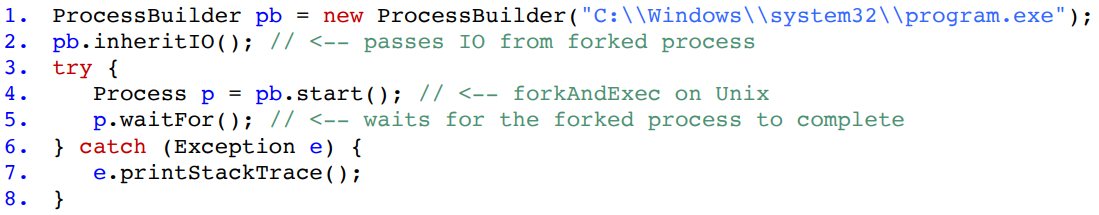
\includegraphics[width = 1\textwidth]{Images/44.PNG}
\end{center}
\subsection{Confronto tra modelli}
Quali caratteristiche hanno quindi i vari modelli presentati? Quando conviene usare uno oppure l'altro?
\begin{itemize}
    \item \textbf{Mono processo (iterativo e concorrente)}
          \begin{itemize}
              \item Gli utenti condividono lo stesso spazio di lavoro
              \item Adatto ad applicazioni \textbf{cooperative} che prevedono la \textbf{modifica dello stato del server} (R/W)
          \end{itemize}
    \item \textbf{Multi processo}
          \begin{itemize}
              \item Ogni utente ha uno spazio di lavoro autonomo
              \item Adatto ad applicazioni cooperative che \textbf{non modificano lo stato del server}
              \item Adatto ad applicazioni \textbf{autonome} che modificano uno spazio di lavoro \textbf{proprio}
          \end{itemize}
\end{itemize}
\section{Concorrenza e Programmazione multithreading}
La \textbf{concorrenza} è la contemporaneità di esecuzione di parti diverse di uno stesso programma (processi, thread a.k.a \textbf{agenti}). È uan caratteristica fondamentale del processo di sviluppo di un software. Due agenti possono essere in esecuzione contemporanea \textbf{anche condividendo la stessa CPU}. Si tengono a distinguere i due seguenti scenari (semplifichiamo):
\begin{itemize}
    \item \textbf{Contemporaneità} di esecuzione su una \textbf{stessa macchina} (con una sola o molte CPU/Core). Gli agenti possono condividere le \textbf{risorse} del S.O.
    \item \textbf{Il programma è in esecuzione su macchine distinte}: le macchine sono collegate tramite una \textbf{rete di comunicazione}. In questo caso, si parla di \textbf{programmazione distribuita}.
\end{itemize}
Gli approcci possibili a questo "modello" di programmazione possono essere:
\begin{itemize}
    \item \textbf{Funzionalità d'ambiente}: \textbf{Meccanismi} che permettono \textbf{l'esecuzione} e la \textbf{comunicazione} tra gli agenti. Sopratutto forniti dal S.O.
    \item \textbf{Funzionalità dei linguaggi di programmazione}: Costrutti di un linguaggio che espandono la programmazione dal \textbf{paradigma sequenziale} a quello \textbf{concorrente/distribuito}
\end{itemize}
\subsection{Concorrenza e Parallelismo}
Possiamo quindi definire la \textbf{concorrenza} come la capacità di \textbf{far eseguire più attività} (processi, thread) \textbf{nel tempo}. Il \textbf{parallelismo} è invece la capacità di \textbf{poter eseguire simultaneamente più attività}. Infatti, un'applicazione \textbf{concorrente ma non parallelizzata} avrebbe, per esempio, questa "coda" di esecuzione:
\begin{center}
    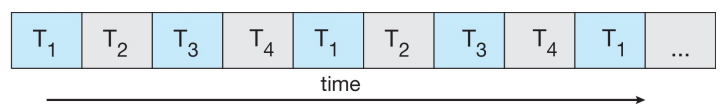
\includegraphics[width = 0.80\textwidth]{Images/45.png}
\end{center}
mentre un'applicazione \textbf{concorrente e parallelizzata} avrebbe, per esempio, questa "coda" di esecuzione:
\begin{center}
    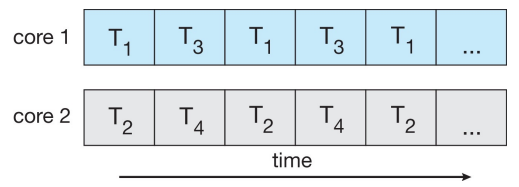
\includegraphics[width = 0.60\textwidth]{Images/46.png}
\end{center}
\subsubsection{Parallelismo dei dati e delle attività}
Il \textbf{parallelismo dei dati} è l'attività di diversi \textbf{core} che eseguono \textbf{la stessa mansione} (quindi eseguono in parallelo attività \textbf{uguali} ma in maniera distinta) operando su \textbf{sottoinsiemi diversi di dati}.
\begin{center}
    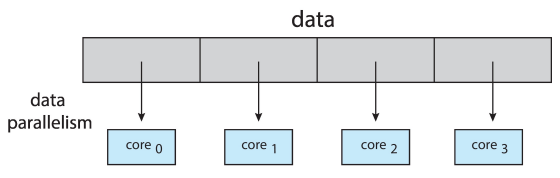
\includegraphics[width = 0.60\textwidth]{Images/47.png}
\end{center}
Il \textbf{parallelismo delle attività} invece è quando \textbf{diversi core} svolgono \textbf{attività diverse} in parallelo, operando su \textbf{dati comuni}.
\begin{center}
    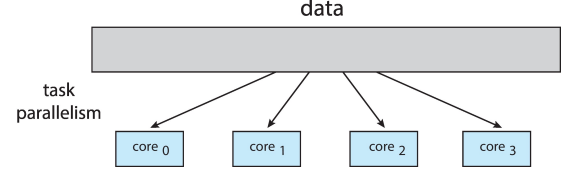
\includegraphics[width = 0.60\textwidth]{Images/48.png}
\end{center}
Questa distinzione tuttavia non deve far pensare che questi due scenari siano \textbf{mutualmente esclusivi}: scenari ibridi sono \textbf{comuni}.

\subsection{Legge di Amdahl}
La legge di Amdahl fornisce \textbf{il guadagno in termini di performance} derivante \textbf{dall'aggiunta di core} ad un'applicazione che ha \textbf{componenti sia sequenziali che parallele}. Sia quindi $S$ la porzione (intesa come tempi di calcolo) di applicazione che deve essere realizzata sequenzialmente e $N$ il numero di core. Allora:
$$incremento \; di \; velocita' \leq \frac{1}{S + \frac{1-S}{N}}$$
Facciamo un esempio: supponiamo che la un'applicazione data sia per il 75\% parallelizzabile. Ciò vuol dire $S = 25\%$. Allora:
\begin{itemize}
    \item Per $N = 2$ abbiamo un'incremento fino a 1,6 volte più veloce di single-core
    \item Per $N = 4$ abbiamo un'incremento fino a 2,24 volte più veloce di single-core
\end{itemize}
\begin{center}
    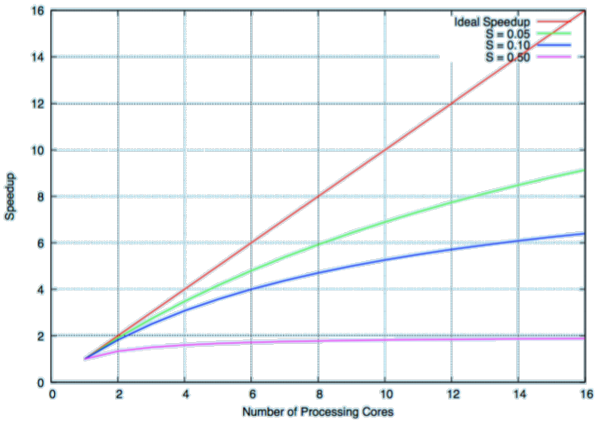
\includegraphics[width = 0.60\textwidth]{Images/49.png}
\end{center}
\subsection{Programmazione concorrente}
Con \textbf{programmazione concorrente} si indica la pratica di implementare dei programmi che \textbf{contengono più flussi di esecuzione} (processi, thread).
\begin{center}
    \includegraphics[width = 0.80\textwidth]{Images/50.png}
\end{center}
Perché è utile creare programmi concorrenti?
\begin{itemize}
    \item Per \textbf{sfruttare tutti i core della CPU}
    \item Per evitare di \textbf{bloccare l'intera esecuzione di un'applicazione} a causa dell'attesa del completamento di un'operazione di I/O
    \item Per sfruttare in modo più adeguato un programma. In particolare programmi che:
          \begin{itemize}
              \item \textbf{Interagiscono} con l'ambiente...
              \item \textbf{Controllano} diverse attività...
              \item \textbf{Gestiscono} eventi diversi..
              \item Magari il tutto mentre \textbf{fornisce servizi} all'utente
          \end{itemize}
\end{itemize}
\subsection{Processi}
Un certo sistema operativo esegue \textbf{un certo numero di programmi} sullo stesso sistema di elaborazione (multi-programmazione). Il numero di questi programmi può essere \textbf{arbitrariamente elevato}, di solito è molto più grande dei core che la CPU mette a disposizione. A tale scopo, il sistema operativo realizza e mette a disposizione \textbf{un'astrazione} detta \textbf{processo}. Un processo è un'\textbf{entità attiva astratta} definita dal S.O. allo scopo di eseguire \textbf{un programma}.
\subsection{Programmi e processi}
È necessario notare la differenza tra \textbf{processo} e \textbf{programma}.
\begin{itemize}
    \item \textbf{Un programma} è un'entità passiva (un insieme di istruzioni tipicamente contenute in un file sorgente o eseguibile)
    \item \textbf{Un processo} è un'entità attiva (è un esecutore di programmi)
          \begin{itemize}
              \item Caricato in memoria è "\textbf{attivato}"
              \item Vengono associate \textbf{strutture ed informazioni} necessarie al funzionamento (es. Stack)
              \item Contiene almeno \textbf{un flusso di controllo di esecuzione} (Thread)
          \end{itemize}
\end{itemize}
Uno stesso programma può \textbf{dare origine a uno o più processi}: diversi utenti possono \textbf{eseguire lo stesso programma} oppure lo stesso utente può \textbf{eseguire più istanze del programma} contemporaneamente.
\subsection{Multiprogrammazione e multitasking}
Tra gli obbiettivi del S.O. vi sono:
\begin{itemize}
    \item \textbf{Massimizzare l'utilizzo della/e CPU}: Mantenere impegnata/e la/e CPU il \textbf{maggior tempo possibile} nell'esecuzione di programmi
    \item \textbf{Dare l'illusione che ogni processo abbia una CPU dedicata}: Astrazione utile agli sviluppatori
\end{itemize}
Due tecniche per raggiungere questi obbiettivi sono la \textbf{multiprogrammazione e il multitasking}:
\begin{itemize}
    \item \textbf{Obbiettivo della multiprogrammazione}: Mantenere in memoria \textbf{più programmi} ed impedire che un programma in attesa di una risorsa (es. operazione di I/O) mantenga il controllo della CPU (\textbf{vecchio concetto}).
    \item \textbf{Obbiettivo del multitasking}: Dare l'illusione del \textbf{parallelismo}. A differenza della multiprogrammazione, il cui task \textbf{utilizza la CPU fino al suo completamento}, in questo modello ogni task ha una \textbf{quantità predeterminata di tempo in cui può usare la CPU}, detta \textbf{quantum}, durante il quale il task può essere eseguito. Notare che questo modello \textbf{non è rilevante per i sistemi puramente batch}, cioè quei sistemi pensati per \textbf{eseguire task sequenzialmente} e in maniera accorpata.
\end{itemize}
\subsubsection{Multiprogrammazione}
Nella multiprogrammazione, il sistema operativo \textbf{mantiene i processi in memoria}: li carica e li assegna una serie di altre informazioni. Quando la CPU non sta eseguendo un processo, il sistema operativo \textbf{sceglie un altro processo non in esecuzione} e lo fa eseguire dalla CPU. Quando un processo \textbf{non può proseguire la sua esecuzione}, cioè quando è in attesa di una risorsa o di un'operazione di I/O, la sua CPU viene \textbf{assegnata ad un altro processo non in esecuzione}.Il risultato di questo modello è che se i processi \textbf{sono più delle CPU}, quest'ultime saranno impegnate nell'esecuzione di un processo per la maggior parte del tempo.
\subsubsection{Multiprogrammazione e memoria}
La multiprogrammazione richiede che \textbf{tutte le immagini di tutti i processi siano in memoria} perché queste possano essere eseguite. Se i processi sono troppi, \textbf{non possono essere tutte contenute in memoria}: si può quindi adottare la tecnica dello \textbf{swapping} per spostare le immagini dei processi dentro e fuori dalla memoria: le immagini dei processi in più \textbf{vengono immagazzinate su un dispositivo di memoria secondaria}. \newline
Altra tecnica per gestire quest'eventualità è la \textbf{memoria virtuale}: essa consiste nella \textbf{completa separazione} tra la \textbf{memoria logica} di un processo e la sua \textbf{memoria fisica}. Con questa tecnica, quindi, un processo \textbf{può essere eseguito anche se la sua immagine non è completamente in memoria}. Al processo viene assegnato \textbf{uno spazio di indirizzamento virtuale}, di solito molto più grande della memoria fisica effettivamente presente; il sistema operativo si occuperà poi di \textbf{tradurre gli indirizzi virtuali in indirizzi fisici}.
\begin{center}
    \includegraphics[width = 0.50\textwidth]{Images/51.PNG}
\end{center}
Queste tecniche di multiprogrammazione \textbf{aumentano il numero di processi che possono essere eseguiti in multiprogrammazione}, cioè aumentano il \textbf{grado di multiprogrammazione} di un sistema.
\subsubsection{Multitasking}
Il multitasking è un'estensione della multiprogrammazione. La CPU viene \textbf{sottratta periodicamente} al programma in esecuzione ed assegnata ad un'altro programma. In questo modello \textbf{tutti i processi progrediscono in maniera continuativa nella loro esecuzione}, anziché solo nei momenti in cui un certo processo \textbf{lascia il controllo della CPU} e si mette in attesa.
Questo permette che i \textbf{programmi batch}, cioè quei programmi che richiedono poche operazione di I/O, non monopolizzino la CPU a scapito dei \textbf{programmi interattivi}.
\subsection{Operazioni sui processi}
I sistemi operativi di solito forniscono delle \textbf{chiamate di sistema}(syscall) con le quali un certo processo può \textbf{creare, terminare o manipolare} altri processi. Dal momento che solo un processo può crearne un altro, all'avvio del sistema operativo, esso crea dei \textbf{processi primordiali} dai quali \textbf{tutti i processi utente e di sistema} derivano.
\subsubsection{Creazione di processi}
Di solito i sistemi operativi organizzano i processi in maniera gerarchica. Un processo \textbf{padre} può creare una serie di \textbf{processi figlio}. Questi, a loro volta, potranno essere i processi padri di altri processi figlio.
\begin{center}
    \includegraphics[width = 0.60\textwidth]{Images/52.PNG}
\end{center}
La relazione gerarchica tra processi è di norma importante per le seguenti politiche:
\begin{itemize}
    \item \textbf{Politiche di condivisione delle risorse}: Padri e figli possono condividere \textbf{tutte} le risorse, un loro \textbf{sottoinsieme} oppure nessuna \textbf{risorsa}.
    \item \textbf{Politiche di creazione dello spazio di indirizzi}: Il figlio è un \textbf{duplicato del padre} (memoria e programma), oppure \textbf{bisogna specificare quale programma deve eseguire il figlio}
    \item \textbf{Politiche di coordinazione}: Il padre può \textbf{sospendersi fino a quando i figli non terminano} oppure eseguono tutti in \textbf{maniera concorrente}
\end{itemize}
\subsubsection{Terminazione dei processi}
I processi, di solito, richiedono esplicitamente la propria \textbf{terminazione} al sistema operativo. Tuttavia, un processo padre può richiedere la \textbf{terminazione di un processo figlio}. Le possibili ragioni per il quale un processo padre vuole terminare forzatamente un suo figlio sono:
\begin{itemize}
    \item Il figlio sta usando \textbf{risorse in eccesso}
    \item Le funzionalità del figlio \textbf{non sono più richieste} (meglio però, in questo caso, una terminazione \textbf{ordinata})
    \item Il padre termina \textbf{prima che i figli terminino}. In particolare, questo dipende dal sistema operativo: alcuni S.O. non permettono che un figlio esista \textbf{dopo la terminazione del padre}, e quindi adottano meccanismi di \textbf{terminazione a cascata} gestiti e iniziati dal S.O.
\end{itemize}
\subsection{Implementazione dei processi}
Un processo è composto da \textbf{diverse parti}:
\begin{itemize}
    \item Lo \textbf{stato} dei registri del processore che esegue il programma, incluso il PC
    \item Lo \textbf{stato} della memoria centrale usata dal programma, detta \textbf{immagine} del processo
    \item Lo \textbf{stato} del processo stesso (new, ready, waiting, running, terminated)
    \item Le \textbf{risorse} del sistema operativo in uso dal programma (files, semafori, regioni di memoria condivisa, ecc...)
\end{itemize}
Processi distinti hanno \textbf{immagini distinte}; mentre le risorse del S.O. possono essere \textbf{condivise} tra processi.
\subsubsection{Immagine di un processo}
L'immagine di un processo è formata da:
\begin{itemize}
    \item Il \textbf{codice} del programma da eseguire (code section)
    \item La \textbf{data section}, contenente le variabili \textbf{globali}
    \item Lo \textbf{stack} delle chiamate, contenete variabili locali, parametri e \textbf{indirizzi di ritorno}
    \item Lo \textbf{heap}, contenete la memoria allocata dinamicamente durante l'esecuzione
\end{itemize}
Code e data section hanno \textbf{dimensioni costanti durante tutta la vita del processo} mentre \textbf{Stack e Heap} hanno dimensioni variabili
\begin{center}
    \includegraphics[width = 0.30\textwidth]{Images/53.PNG}
\end{center}
\subsubsection{Stato di un processo}
Durante l'esecuzione di un processo, esso cambia \textbf{più volte stato}. Gli stati possibili sono:
\begin{itemize}
    \item \textbf{New}: Il processo è stato creato, ma non è ancora in esecuzione
    \item \textbf{Ready}: Il processo è pronto per essere eseguito, ma non gli è stata ancora assegnata una CPU
    \item \textbf{Running}: Il processo è in esecuzione
    \item \textbf{Waiting}: Il processo non può continuare la sua esecuzione poiché \textbf{è in attesa di un evento o di un operazione di I/O}
    \item \textbf{Terminated}: Il processo è stato terminato
\end{itemize}
\begin{center}
    \includegraphics[width = 0.65\textwidth]{Images/54.PNG}
\end{center}
\subsubsection{PCB: Process Control Block}
Detto anche \textbf{Task Control Block}, il \textbf{Process Control Block} (PCB) è la \textbf{struttura dati} del kernel che contiene tutte le informazioni riguardanti un processo. Essa contiene:
\begin{itemize}
    \item \textbf{Process state}: lo stato del processo
    \item \textbf{Process number}: il PID (Process IDentifier) del processo
    \item \textbf{Program Counter}: Contenuto del registro PC
    \item \textbf{Registers}: Contenuto dei registri del processore
    \item \textbf{Informazioni sulla memoria allocata}
    \item \textbf{Informazioni sull'I/O}: dispositivi assegnati, file aperti,...
    \item \textbf{Informazioni di Scheduling}: Priorità, puntatori a code di scheduling, ...
    \item \textbf{Informazioni di accounting}: CPU utilizzata, tempo trascorso, ...
\end{itemize}
\begin{center}
    \includegraphics[width = 0.30\textwidth]{Images/55.PNG}
\end{center}
\subsection{Scheduling dei processi}
Lo scheduler dei processi sceglie \textbf{quale processo eseguire} tra quelli in stato di \textbf{ready}.
\begin{center}
    \includegraphics[width = 0.65\textwidth]{Images/56.PNG}
\end{center}
Esso mantiene diverse code:
\begin{itemize}
    \item \textbf{Ready queue}: Processi residenti in memoria e in stato di \textbf{ready}
    \item \textbf{Wait queues}: Code per processi residenti in memoria ma in stato di \textbf{wait}, una queue per ogni evento di attesa
\end{itemize}
Durante la loro vita, i processi e i loro PCB, migrano \textbf{da una coda all'altra} a seconda dello stato del processo stesso.
\subsection{Commutazione di contesto}
\begin{center}
    \includegraphics[width = 0.60\textwidth]{Images/57.PNG}
\end{center}
Quando la CPU deve passare dall'esecuzione di un processo a quella di un altro processo avviene una \textbf{commutazione di contesto} (context switch); essa viene eseguita dal \textbf{dispatcher}, che:
\begin{itemize}
    \item Salva il contesto (stato, registri,...) del processo da interrompere nel suo PCB
    \item Carica il contesto del processo da eseguire dal suo PCB
\end{itemize}
Il tempo necessario ad eseguire un context switch \textbf{è overhead}: non viene eseguito alcun lavoro utile. Da notare che più complesso è il S.O., più è complesso il context switch, più tempo serve per farlo. Alcuni processori offrono \textbf{supporto hardware speciale} per ridurre il tempo dei context switch.
\subsection{Comunicazione interprocesso (IPC)}
I processi possono essere \textbf{indipendenti} oppure possono \textbf{cooperare}. Un processo coopera se il suo comportamento è \textbf{influenzato} oppure \textbf{influenza} altri processi. Ci sono più motivi per volere processi cooperanti:
\begin{itemize}
    \item Condivisione di \textbf{informazioni}
    \item \textbf{Accelerazione} delle computazioni
    \item Modularità e \textbf{isolamento} (Chrome)
\end{itemize}
Per permettere ai processi di comunicare, il sistema operativo deve mettere a disposizione delle \textbf{primitive di comunicazione interprocesso} (IPC).
\subsubsection{IPC tramite memoria condivisa}
\begin{center}
    \includegraphics[width = 0.30\textwidth]{Images/58.PNG}
\end{center}
In questo modello, \textbf{viene stabilita una zona di memoria condivisa} che i processi usano per comunicare. La comunicazione è \textbf{controllata dai processi che comunicano} e non dal sistema operativo. Un problema importante è \textbf{la sincronizzazione} tra questi diversi processi; i sistemi operativi mettono a disposizione \textbf{primitive apposite} per la sincronizzazione.
\newpage
\subsubsection{IPC tramite message passing}
\begin{center}
    \includegraphics[width = 0.30\textwidth]{Images/59.PNG}
\end{center}
In questo modello, \textbf{viene permesso ai processi sia di comunicare che di sincronizzarsi}. I processi comunicano tra loro \textbf{senza condividere memoria} attraverso la mediazione del S.O. o di un altro processo. Devono essere quindi disponibili:
\begin{itemize}
    \item Un'operazione di \textbf{send(message)} per l'invio di un messaggio tra un processo e l'altro
    \item Un'operazione di \textbf{receive(message)} con la quale un processo ascolta (eventualmente mettendosi in attesa) e riceve i messaggi degli altri processi.
\end{itemize}
Quindi per comunicare, i due processi devono \textbf{stabilire un link di comunicazione} tra loro e passarsi messaggi. Questo tipo di comunicazione è la normalità nella \textbf{programmazione distribuita}.
\subsection{Multithreading}
Se supponiamo che un processo possa avvalersi di \textbf{molte CPU} contemporaneamente, allora una sua serie di istruzioni possono essere eseguite \textbf{contemporaneamente}; quindi un processo può avere \textbf{più flussi di esecuzione concorrenti} (threads). I threads (\textbf{lightweight processes)} quindi sono stati introdotti per tale scopo. I thread di un processo condividono:
\begin{itemize}
    \item La \textbf{memoria globale} (data e heap)
    \item La \textbf{code section}
    \item Le \textbf{risorse ottenute dal S.O.} (es. file aperti)
\end{itemize}
Tuttavia, ogni thread deve avere \textbf{un proprio stack di chiamate}, altrimenti le chiamate effettuate da un thread andrebbero a interferire con quelle di altri thread concorrenti.
\begin{center}
    \includegraphics[width = 0.30\textwidth]{Images/60.PNG}
\end{center}
Un programma \textbf{sequenziale} (single-threaded) ha un singolo flusso di controllo; si crea quindi un processo con un \textbf{flusso unico}.
\begin{center}
    \includegraphics[width = 0.35\textwidth]{Images/61.PNG}
\end{center}
Un programma \textbf{multi-threaded} ha più flussi di esecuzione che gli permettono di \textbf{svolgere più mansioni allo stesso tempo}. Molto spesso, tuttavia, \textbf{i thread di un programma devono sincronizzarsi}
\subsection{Thread Control Blocks (TCB)}
Nei kernel multithreaded, vengono mantenute delle strutture dati analoghe ai PCB, i \textbf{Thread Control Blocks} (TCB); un TCB memorizza il contesto del thread e le sue informazioni di contabilizzazione. Il PCB di un processo \textbf{raccoglie solamente le informazioni di contabilizzazione comuni} (es. lo spazio di memoria) ed è di solito collegato ai TCB dei \textbf{thread kernel}, e viceversa, i TCB dei thread kernel utilizzati da un processo sono collegati al suo PCB.
\subsection{Vantaggi del multithreading e sfide}
Il multithreading può portare a diversi vantaggi:
\begin{itemize}
    \item \textbf{Condivisione di codice e dati}: i thread di un processo condividono lo \textbf{stesso spazio di memoria} e lo stesso codice
    \item \textbf{Economia}: Creare un thread richiede meno risorse che creare un processo, inoltre il cambio di contesto è \textbf{più rapido}
    \item \textbf{Migliori tempi di risposta}: L'applicazione può eseguire un compito lungo \textbf{in un thread separato} e comunque rispondere e offrire servizi all'utente
    \item \textbf{Scalabilità}: Il multithreading in una macchina con più processi aumenta il \textbf{grado di parallelismo} di un'applicazione
    \item \textbf{Ottimizzazione delle risorse}: Se un thread è in attesa di una operazione di I/O, un'altro thread può accedere alla CPU \textbf{evitando il context switch} dell'intero processo
\end{itemize}
Tuttavia presenta anche delle sfide:
\begin{itemize}
    \item \textbf{Identificazione} dei compiti da eseguire dai vari thread
    \item \textbf{Bilanciamento} in maniera tale che i compiti eseguiti dai vari thread abbiano dimensione di attività confrontabili
    \item \textbf{Suddivisione} dei dati per massimizzare l'accesso in parallelo
    \item \textbf{Dipendenza} trai dati prodotti/consumati dai vari thread, per stabilire la sincronizzazione
    \item \textbf{Testing} e \textbf{Debugging}
\end{itemize}
\subsection{Implementazione del multithreading}
I thread possono essere:
\begin{itemize}
    \item \textbf{Thread a livello utente}: i thread disponibili nello spazio utente dei processi; son quelli offerti dalle librerie di thread ai processi (logici)
    \item \textbf{Thread a livello kernel}: I thread implementati nativamente dal kernel; sono utilizzati per sfruttare \textbf{il kernel stesso} in maniera concorrente (reali)
\end{itemize}
I thread a livello del kernel vengono usati dalle librerie per \textbf{creare i thread a livello utente di un certo processo} (avviene quindi una commutazione di contesto). A tale scopo possono adottare diverse strategie.
\subsubsection{Molti a uno}
\begin{center}
    \includegraphics[width = 0.45\textwidth]{Images/62.PNG}
\end{center}
In questo modello, i thread di un singolo processo sono \textbf{implementati su un solo thread a livello kernel}. Il vantaggio di questo modello è che \textbf{è usabile su ogni S.O.}, anche quelli con kernel non multithreaded. Tuttavia, se un thread fa una chiamata di sistema bloccante, \textbf{blocca tutti gli altri thread} del processo, inoltre non sfrutta la presenza di più core.
\subsubsection{Uno a uno}
\begin{center}
    \includegraphics[width = 0.45\textwidth]{Images/63.PNG}
\end{center}
Ogni singolo thread a livello utente è implementato su un \textbf{singolo, distinto} thread a livello kernel. Il vantaggio di questo modello è che \textbf{permette un maggior grado di concorrenza} e di sfruttare il \textbf{parallelismo} dei sistemi multicore. Tuttavia \textbf{è un modello pesante da sostenere} per il kernel e presente un \textbf{maggior overhead}.
\subsubsection{Molti a molti}
\begin{center}
    \includegraphics[width = 0.45\textwidth]{Images/64.PNG}
\end{center}
I thread a livello utente di un certo processo sono \textbf{implementati su un insieme di thread a livello kernel}, possibilmente inferiori di numero. L'associazione thread utente-thread kernel è \textbf{dinamica}, stabilita da uno \textbf{scheduler interno alla libreria dei thread}. Questo modello cerca quindi di combinare i vantaggi dei modelli precedenti. Tuttavia è \textbf{complesso da implementare}: la libreria dei thread deve \textbf{dinamicamente alternare} l'esecuzione dei thread a livello utente sui thread a livello del kernel. È possibile implementare anche un \textbf{modello a due livelli} che permette agli utenti di creare threads con mapping uno-a-uno con un \textbf{thread a livello del kernel}.
\subsubsection{Comunicazione tra libreria dei thread e scheduler dei thread del kernel}
Nel caso del modello \textbf{molti-a-molti}, mantenere il mapping tra threads a livello utente e thread a livello del kernel \textbf{è difficile}. Un problema in particolare è la \textbf{comunicazione} tra la \textbf{libreria} dei thread a livello utente e lo \textbf{scheduler} dei thread a livello kernel: entrambi infatti \textbf{prendono decisioni di scheduling}, quindi devono collaborare. Presentiamo quindi alcune astrazioni per farlo.
\subsubsection{Lightweight process (LWP)}
Un \textbf{lightweight process} (LWP) è \textbf{l'interfaccia} che il kernel offre alla libreria dei thread per usare i thread a livello del kernel. Ogni LWP è un oggetto astratto associato dal kernel a \textbf{esattamente un thread a livello del kernel}. La libreria dei thread può usare un LWP per mandare in esecuzione un thread utente però L'LWP può \textbf{bloccarsi} o essere \textbf{preempted} dal kernel. Un LWP può essere inoltre usato dalla libreria per \textbf{aggiornare le minime informazioni relative al contesto del processo utente utili a prendere migliori decisioni di scheduling}.
\begin{center}
    \includegraphics[width = 0.45\textwidth]{Images/65.PNG}
\end{center}
\subsubsection{Attivazione dello scheduler}
L'attivazione dello scheduler è un modello di \textbf{collaborazione tra libreria dei thread e kernel}. Il kernel comunica alla libreria dei thread \textbf{l'occorrenza dei principali eventi di scheduling sugli LWP attraverso upcall}; quest'ultime \textbf{chiamano opportune funzioni di callback alla libreria dei thread}. In risposta ad una callback, la libreria dei thread può:
\begin{itemize}
    \item Aggiornare le proprie strutture dati (es. registrare che un certo thread è bloccato)
    \item Decidere di effettuare operazioni di scheduling (es. continuare l'esecuzione di un thread preempted assegnandolo un altro di LWP)
\end{itemize}
\begin{center}
    \includegraphics[width = 0.55\textwidth]{Images/66.PNG}
\end{center}
\subsection{Multithreading in Java}
I \textbf{Java Threads} sono astrazioni offerte dalla \textbf{JVM} (Java Virtual Machine) e gestite dalla stessa. Essi vengono tipicamente implementati \textbf{seguendo il modello di threading offerto dal sistema operativo sottostante}, ma la JVM non fornisce uno standard specifico. La JVM quindi offre una \textbf{libreria} per la definizione dei thread e per la loro interazione con il S.O. per la loro esecuzione. Vi sono due modi per creare un thread in java:
\begin{enumerate}
    \item Usare un oggetto di una classe che estende \textbf{java.lang.Thread}
    \item (Preferibile) Implementare una classe che \textbf{implementa java.lang.Runnable} e il suo metodo \textbf{run()}
\end{enumerate}
In Java, ogni programma in esecuzione \textbf{è un thread}. Il metodo main di ogni programma java è associato al \textbf{thread "main"}. Per poter accedere alle proprietà del thread in esecuzione è necessario ottenere un riferimento tramite il metodo \newline \textbf{currentThread()}.
\begin{center}
    \includegraphics[width = 1.10\textwidth]{Images/67.PNG}
\end{center}
\subsubsection{La classe principale per i thread Java}
I modi più semplici in Java per creare un Thread sono:
\begin{enumerate}
    \item Estendere la classe \textbf{java.lang.Thread} che contiene un metodo \textbf{run()} vuoto.
          \begin{center}
              \includegraphics[width = 0.70\textwidth]{Images/68.PNG}
          \end{center}
    \item Effettuare \textbf{l'override} del metodo \textbf{run()} nella sottoclasse. Il codice eseguito dal thread è incluso nel metodo run() e nei metodi invocati indirettamente o direttamente da esso. Questo codice verrà quindi eseguito da ogni thread che viene fatto partire da questa sottoclasse
    \item Creare un'istanza della sottoclasse
    \item Richiamare il \textbf{metodo start()} su quest'istanza
          \begin{itemize}
              \item \textbf{Pattern}: Spesso si estende il costruttore in modo che \textbf{invochi il metodo start()}: in tal modo creare l'istanza della classe fa partire anche il thread.
          \end{itemize}
\end{enumerate}
\subsubsection{Far partire i thread in java}
Una chiama del tipo \textbf{t.start()} rende il thread t \textbf{pronto} (ready) all'esecuzione. Prima o poi, quando lo scheduler lo riterrà opportuno, il thread \textbf{verrà mandato in esecuzione} e verrà invocato il metodo run() del thread t. I due thread, \textbf{creante e creato}, saranno eseguiti in maniera \textbf{indipendente e concorrente}. Bisogna notare che, seppur l'ordine delle operazioni di ogni thread è noto, \textbf{l'ordine di esecuzione dei thread è ignoto} (nondeterminismo)
\subsubsection{Runnable interface}
Siccome Java non consente l'ereditarietà multipla, un altro metodo per implementare un thread è \textbf{implementare l'interfaccia Runnable} ed farne l'override del metodo \textbf{run()}. Ciò ci permette di \textbf{estendere un'altra classe} al posto di Thread. La classe base \textbf{Thread} può essere \textbf{inizializzata con un oggetto Runnable}, del quale utilizzerà il metodo run() una volta dato lo start.
\begin{center}
    \includegraphics[width = 0.70\textwidth]{Images/69.PNG}
\end{center}
Quindi per implementare un thread in questo modo dobbiamo:
\begin{enumerate}
    \item Definire una classe che implementa \textbf{Runnable} e fare l'override del metodo \textbf{run()}
    \item Creare un'istanza di quella classe
    \item Creare una nuova istanza di \textbf{Thread} passando al costruttore l'istanza della classe che implementa Runnable
    \item Chiamare il metodo start() sull'oggetto \textbf{Thread}
\end{enumerate}
\begin{center}
    \includegraphics[width = 0.75\textwidth]{Images/70.PNG}
\end{center}
\subsubsection{Stato di un thread}
L'invocazione del metodo start() porta il \textbf{Thread} ad eseguire il metodo run(). Un thread è considerato \textbf{alive} fino a quando run() non termina e ritorna, dopodiché viene considerato \textbf{terminated}. Una volta che un thread è stato terminato \textbf{NON PUÒ} essere rieseguito; se ci si prova, Java lancia una \textbf{IllegalThreadStateException}.
\begin{center}
    \includegraphics[width = 0.80\textwidth]{Images/71.PNG}
\end{center}
Il predicato \textbf{isAlive()} permette di sapere se il thread corrente è stato terminato oppure se il suo metodo run() è ancora in esecuzione.
\subsubsection{Diagramma degli stati di un thread}
Quando chiamiamo il metodo \textbf{start()} su un thread, esso non viene eseguito immediatamente, ma passa nello \textbf{stato di Ready}. Quando lo scheduler lo riterrà opportuno, il thread viene selezionato dalla coda e passa nello stato di \textbf{Running} ed esegue il metodo \textbf{run()}.
\begin{center}
    \includegraphics[width = 0.75\textwidth]{Images/72.PNG}
\end{center}
Come funziona effettivamente lo scheduler \textbf{dipende dalla piattaforma su cui si trova la JVM}. In generale:
\begin{itemize}
    \item Lo scheduling avviene in maniera \textbf{preempted} e \textbf{priority based}
    \item I thread Java sono provvisti di \textbf{priorità} e il thread con la priorità più alta sarà quello che verrà schedulato tra tutti i thread in stato di Ready.
    \item Con il diritto di \textbf{preemption} lo scheduler può \textbf{sottrarre la CPU al processo} che la sta usando per assegnarla ad un altro processo
\end{itemize}
Poiché ad ogni thread è assegnato un \textbf{quanto di tempo} d'uso della CPU, \textbf{yield()} fornisce un meccanismo per informare lo scheduler che il thread è \textbf{disposto a cedere la CPU} ma che vorrebbe essere rischedulato il prima possibile. Lo scheduler è tuttavia libero \textbf{ignorare o di prendere in considerazione} questa informazione; ciò dipende dal S.O.
\begin{center}
    \includegraphics[width = 0.60\textwidth]{Images/73.PNG}
\end{center}
\subsubsection{Rallentare un thread: sleep(mill)}
Per rallentare l'esecuzione di un thread, potremmo implementare un metodo che \textbf{giri a vuoto} (busy loop). Tuttavia questa soluzione è \textbf{inefficiente}: si sprecano cicli di processore quando essi potrebbero essere impegnati in qualche attività utile. Inoltre, se ci sono molti threads, è possibile che quando si arriva al momento il thread esce dal ciclo \textbf{esso non abbia accesso alla CPU}, quindi si rischia di \textbf{rallentarlo più di quanto previsto}. La soluzione è il metodo \textbf{sleep(mill)}, che \textbf{ferma l'esecuzione del thread per un tempo uguale a mill}. Il metodo \textbf{libera la CPU}, è statico e \textbf{non spreca cicli del processore}; tuttavia và gestita la \textbf{InterruptedException} che questo metodo invoca nel caso il thread in pausa riceva una \textbf{richiesta di interruzione} ma esso non abbia accesso alla CPU.
\subsubsection{Cancellare un thread}
Cancellare un thread significa \textbf{terminarne l'esecuzione prima del previsto}. Ci sono due possibili modelli di cancellazione:
\begin{itemize}
    \item \textbf{Cancellazione immediata}: Il thread è terminato immediatamente
    \item \textbf{Cancellazione differita}: Il thread controlla periodicamente se deve terminare, in modo da effettuare una terminazione \textbf{ordinata} (è il caso di Java)
\end{itemize}
In java il metodo \textbf{interrupt()} è il modo predefinito per terminare un thread. Il metodo imposta una \textbf{flag di interruzione del thread} di destinazione e ritorna. Tuttavia, il thread che riceve l'interrupt \textbf{non viene effettivamente interrotto}, ma esso \textbf{deve controllare periodicamente che non sia arrivata nessuna richiesta di interrupt}. Per farlo ha due metodi:
\begin{itemize}
    \item \textbf{isInterrupted()}: controlla se la flag d'interruzione è settata
    \item \textbf{interrupted()}: controlla se la flag d'interruzione è settata \textbf{e la pulisce} (la riporta a 0)
\end{itemize}
Ad ogni chiamata dei metodi \textbf{sleep, join, ecc...} la flag d'interruzione \textbf{viene controllata automaticamente}. Se un thread tuttavia è in \textbf{pausa} quando riceve un interrupt, la JVM si accorge di questa eventualità e si occupa di \textbf{risvegliare il thread} lanciando una \textbf{InterruptedException}; il thread dovrà quindi \textbf{gestire questa eventualità} in modo da terminare ordinatamente.
\begin{center}
    \includegraphics[width = 1\textwidth]{Images/74.PNG}
\end{center}
Ovviamente \textbf{interrupt()} non funziona se i thread \textbf{non compiono mai attese}, quindi è necessario che essi \textbf{controllino periodicamente che non siano arrivate richieste di interrupt}.
\subsection{Threading implicito}
Il \textbf{threading implicito} è un meccanismo che \textbf{delega la creazione e gestione dei threads ai compilatori e alle librerie}. L'obbiettivo è permette agli sviluppatori di \textbf{pensare in termini di task da compiere e da mappare su thread}, che verranno poi creati e gestiti automaticamente. Alcuni approcci a questo meccanismo sono:
\begin{itemize}
    \item \textbf{Gruppi di threads} (Thread pools)
    \item \textbf{Fork-join}
    \item \textbf{OpenMP} (non argomento di questo corso)
    \item \textbf{Grand Central Dispatch} (non argomento di questo corso)
    \item \textbf{Intel Threading Building Blocks} (non argomento di questo corso)
\end{itemize}
\subsubsection{Thread pools}
L'idea di questo meccanismo è che \textbf{viene creato un certo numero di thread}, organizzati in gruppo, che attendono di \textbf{rispondere ad una richiesta di lavoro}. Un sistema intelligente quindi \textbf{assegna ad ogni thread un lavoro da svolgere}. Questo meccanismo viene usato per la gestione del ciclo di vita delle \textbf{servlet}. I vantaggi sono:
\begin{itemize}
    \item Più rapido che creare un nuovo thread all'arrivo della richiesta
    \item Il numero di thread esistenti è limitato dalla dimensione del pool
    \item Separa il task da svolgere dal meccanica della sua creazione, permettendo \textbf{diverse strategie di esecuzione} (periodica, in ritardo, ...)
\end{itemize}
In Java, una thread pool può essere "creata" tramite la classe \textbf{ExecutorService}; questa classe mette a disposizione una serie di metodi per gestire i thread della thread pool e per assegnarli delle task. Gli oggetti generici \textbf{Future<>} permettono di rappresentare dei \textbf{segnaposto} dove i risultati delle task verranno immagazzinati. Questo, seppur permetta di effettuare computazioni nell'attesa, richiede quindi di effettuare un'operazione di \textbf{polling} (richieste continue - while) per controllare che il risultato sia pronto. Dietro le quinti di tutto ciò \textbf{lavorano sempre i thread}, ma vengono gestiti in maniera \textbf{trasparente dalla JVM}.
Presentiamo un esempio:
\begin{center}
    \includegraphics[width =9.25cm]{Images/75.PNG}
\end{center}
\begin{center}
    \includegraphics[width = 0.70\textwidth]{Images/76.PNG}
\end{center}
\subsubsection{Fork-Join}
Il modello \textbf{fork-join} consiste nel dividere il problema in \textbf{sottoproblemi eseguibili da threads}; ricorda quindi molto il modello \textbf{dividi-et-impera} di alcuni algoritmi ricorsivi. Lo pseudocodice per questo modello può essere scritto nel seguente modo:
\begin{center}
    \includegraphics[width = 0.80\textwidth]{Images/77.PNG}
\end{center}
Presentiamo un esempio:
\begin{center}
    \includegraphics[width = 0.80\textwidth]{Images/78.PNG}
\end{center}
\begin{center}
    \includegraphics[width = 0.80\textwidth]{Images/79.PNG}
\end{center}
\begin{center}
    \includegraphics[width = 0.80\textwidth]{Images/80.PNG}
\end{center}
\newpage
\section{Thread e Sincronizzazione}
I programmi concorrenti hanno delle proprietà diverse rispetto ai programmi sequenziali. Un programma \textbf{sequenziale}(deterministico) eseguito ripetutamente con lo stesso input \textbf{produce sempre lo stesso risultato}; eventuali errori saranno quindi \textbf{riproducibili}. Tuttavia lo stesso \textbf{non vale per i programmi concorrenti}, in cui il comportamento di un thread \textbf{può influenzare quello degli alti thread} in maniera \textbf{non deterministica}. È necessario quindi che gli agenti concorrenti interagiscano:
\begin{itemize}
    \item \textbf{Cooperazione}: interazioni prevedibili e desiderate. La loro presenza è necessaria per la logica del programma. Avviene tramite scambio di informazioni (anche semplici come segnali); questo è il caso della \textbf{sincronizzazione diretta o esplicita} dei threads
    \item \textbf{Competizione}: gli agenti competono per accedere ad una risorsa condivisa. Politiche di accesso alla risorsa sono necessarie. Questo è il caso della \textbf{sincronizzazione indiretta o implicita}
    \item \textbf{Interferenze}: : interazioni ”non prevedibili e non desiderate”, come \textbf{errori di programmazione}, spesso dipendenti dalle tempistiche (time dependent) e non facilmente riproducibili.
\end{itemize}
\subsection{Meccanismi di sincronizzazione}
I meccanismi di sincronizzazione permettono di \textbf{controllare l’ordine relativo} delle varie attività dei processi/thread. Se si implementa un modello di memoria \textbf{condivisa}, essi possono essere:
\begin{enumerate}
    \item \textbf{Mutua esclusione}: I dati, attraverso la creazione di \textbf{regioni critiche} del codice, non sono accessibili contemporaneamente a più thread
    \item \textbf{Sincronizzazione su condizione}: si sospende l’esecuzione di un thread fino al \textbf{verificarsi di una opportuna condizione} sulle risorse condivise
\end{enumerate}
Se si implementa invece un modello basato sullo \textbf{scambio di messaggi}:
\begin{enumerate}
    \item I meccanismi sono di solito \textbf{impliciti nelle primitive send e receive}, cioè un thread può ricevere un messaggio solo dopo il suo invio
    \item \textbf{Sincronizzazione su eventi}: si sospende l’esecuzione di un thread \textbf{fino al verificarsi di un evento}
\end{enumerate}
Questi meccanismi vengono messi a disposizione dal sistema operativo. In Java ritroviamo le stesse
soluzioni implementate a livello di JVM per i thread.
\subsubsection{Sincronizzazione su eventi: join()}
Questo meccanismo è un \textbf{esempio di sincronizzazione temporale} tra due thread.
\begin{center}
    \includegraphics[width = 0.30\textwidth]{Images/81.PNG}
\end{center}
In java, il metodo \textbf{join()} è definito nella classe \textbf{Thread}. Quando si invoca il metodo \textbf{join()} su un thread, il thread chiamante entra in uno stato di \textbf{attesa} (wait). Rimane in tale stato finché il thread chiamato (t1) non termina. § Il metodo join() può anche ritornare se il thread chiamato viene \textbf{interrotto}. In questo caso, il metodo lancia una \textbf{InterruptedException} che dovrà essere gestita dal thread. Infine, se il thread chiamato è \textbf{già terminato} o \textbf{non è stato avviato}, la
chiamata al metodo join() \textbf{ritorna immediatamente}.
\subsubsection{Sincronizzazione su eventi: Barriere}
In questo modello, i thread vengono \textbf{messi progressivamente in attesa} fin a quando \textbf{una condizione globale non viene soddisfatta}. Una possibile implementazione di questo meccanismo è il seguente:
\begin{itemize}
    \item \textbf{Un contatore condiviso} conta il numero di processi che devono terminare
    \item \textbf{Il contatore decrementa} ogni volta che un thread finisce la sua task
    \item Aggiornamento del \textbf{contatore atomico}
\end{itemize}
\begin{center}
    \includegraphics[width = 0.60\textwidth]{Images/82.png}
\end{center}
\subsection{Problematiche di sincronizzazione: Race Condition}
Nei programmi concorrenti, molti problemi sono causati dalle \textbf{corse critiche} (Race condition), cioè tutte quelle situazioni in cui thread diversi \textbf{operano su una risorsa comune} ed il cui risultato viene a dipendere \textbf{dall'ordine} in cui i thread eseguono. Questo problema avviene a causa della \textbf{competizione per l'accesso ad una risorsa condivisa}, come una variabile in memoria. Il problema è causato dal fatto che certe azioni di un thread, come la lettura/scrittura, \textbf{non sono atomiche} e quindi sono \textbf{interrompibili dallo scheduler}. Un aggiornamento incorretto di una risorsa a causa di una combinazione \textbf{aleatoria} di letture e scritture viene detto \textbf{interferenza}. Per evitare questo problema, esistono diverse soluzioni:
\begin{itemize}
    \item \textbf{Attesa attiva} (busy waiting):
          \begin{itemize}
              \item Ha senso in solo in sistemi \textbf{multiprocessore}
              \item Non richiede commutazione di contesto
              \item Spreca cicli di calcolo della CPU
              \item Consiste nel \textbf{verificare che una certa condizione sia verificata}
          \end{itemize}
    \item \textbf{Sincronizzazione basata sullo scheduler}
          \begin{itemize}
              \item (auto-)sospensione del thread
              \item Il thread viene risvegliato una volta \textbf{che l'evento atteso} si verifica.
          \end{itemize}
\end{itemize}
In java, l'implementazione dipende dalla particolare JVM e dall'ottimizzatore.
\subsubsection{Sincronizzazione basata su sezione critica}
La \textbf{sezione critica} è un blocco di codice che può essere eseguito \textbf{da un solo thread alla volta}. L'obbiettivo quindi è quello di realizzare \textbf{una mutua esclusione}, cioè stabilire un protocollo tra i processi che faccia in modo che quando un thread si trova nella sezione critica \textbf{gli altri non lo siano}.
\begin{itemize}
    \item \textbf{Protocollo}: ogni thread accede alla risorsa condivisa (accessibile tramite sezione critica) mediante le seguenti operazioni:
          \begin{enumerate}
              \item \textbf{Sezione di ingresso}: richiesta di entrata nella sezione critica
              \item \textbf{Sezione critica}
              \item Eventuale \textbf{sezione di uscita} (ad esempio, la notifica agli altri processi)
          \end{enumerate}
\end{itemize}
Per realizzare questo protocollo, abbiamo bisogno di un'operazione non interrompibile (atomica) \textbf{test\_and\_set(B)} (con B una variabile booleana) che ritorna \textbf{il contenuto originale della cella di memoria puntata e imposta il valore della cella a true}. Vediamo come realizzare il protocollo.
\subsubsection{Lock}
Il \textbf{lock} è una variabile \textbf{logica} manipolabile \textbf{atomicamente}:
\begin{itemize}
    \item È una variabile \textbf{binaria}
    \item Due metodi \textbf{lock()} e \textbf{unlock()} permettono di acquisire e rilasciare il lock in maniera \textbf{atomica}
    \item Una volta che un thread acquisisce un lock, \textbf{gli altri thread si arrestano} fino a quando il thread \textbf{non rilascia il lock}.
    \item \textbf{Per ogni lock} deve essere gestita una coda di thread in attesa.
\end{itemize}
In java, le implementazioni dei lock sono disponibili in \textbf{java.lang.concurrent.locks}; in particolare i metodi \textbf{lock()} e \textbf{unlock()} devono essere invocati rispettivamente \textbf{all'inizio e alla fine di ogni sezione che si vuole dichiarare critica}.
\subsubsection{Semaforo}
Un semaforo è una variabile \textbf{intera} che può essere manipolata \textbf{atomicamente} solo tramite le operazioni \textbf{acquire()} e \textbf{release()}: la prima \textbf{aspetta che la variabile sia maggiore di 0 e poi la decrementa}, la seconda \textbf{incrementa incondizionatamente la variabile}. Per ogni semaforo \textbf{è necessario gestire una coda di thread in attesa}. Come per i lock, \textbf{acquire()} e \textbf{release()} sono da invocare rispettivamente \textbf{all'inizio e alla fine di ogni sezione che si vuole dichiarare critica}. I semafori in Java sono presenti in \textbf{java.lang.concurrent.semaphore}
\subsubsection{Mutua esclusione implicita in oggetti Java: metodi Synchronized}
L'attivazione di un certo metodo può essere resa \textbf{mutualmente esclusiva} tramite la specifica della keyword \textbf{synchronized}. Java associa un \textbf{un lock implicito} (un semaforo binario) ad ogni oggetto che abbia almeno \textbf{un metodo synchronized}. Poiché ogni oggetto estende la classe Object, ogni oggetto \textbf{ha un suo lock} (Java Language Specification 17.1). In particolare:
\begin{itemize}
    \item 1 oggetto = 1 lock se c'è almeno un metodo \textbf{synchronized}
    \item L'oggetto con il metodo synchronized \textbf{è la risorsa condivisa tra i thread}
    \item \textbf{synchronized} non può essere usati su singoli campi oppure sui costruttori
\end{itemize}
Quando un metodo synchronized viene invocato:
\begin{itemize}
    \item Se l'oggetto non è \textbf{bloccato} (ovvero nessun thread sta eseguendo un metodo synchronized sull'oggetto), esso viene bloccato e il metodo viene eseguito.
    \item Se l'oggetto è \textbf{bloccato}, il thread \textbf{viene messo in attesa fino a quando il lock non viene rilasciato}.
\end{itemize}
Possiamo quindi rivedere il diagramma di stato dei thread:
\begin{center}
    \includegraphics[width = 0.70\textwidth]{Images/83.png}
\end{center}
La parola chiave \textbf{synchronized} tuttavia implica certe conseguenze:
\begin{itemize}
    \item L'introduzione di \textbf{synchronized} nella dichiarazione dei metodi di una risorsa condivisa \textbf{forza} un \textbf{ordinamento nell'esecuzione} di questi metodi da parte di \textbf{thread concorrenti}
    \item Quanto un metodo synchronized termina, si stabilisce automaticamente una relazione di \textbf{happens-before} con ogni invocazione successiva di alti metodi synchronized sullo stesso oggetto
    \item Ai fini delle problematiche di interferenza, è come se questi metodi fossero stati resi \textbf{atomici}
    \item L'acquisizione e il rilascio dei lock intrinsechi \textbf{viene gestito completamente dalla JVM} ed è \textbf{trasparente} al programmatore
\end{itemize}
È possibile dichiarare anche solo \textbf{parti di metodi synchronized} usando la dichiarazione \textbf{synchronized(Object) \{...\}}. Ciò dichiara che un certo blocco di codice \textbf{è sincronizzato in relazione ad un determinato oggetto}(tipicamente \textbf{this}). \newline
I metodi \textbf{synchronized} danno accesso \textbf{esclusivo} ai dati incapsulati in un oggetto \textbf{solo se a tali dati è possibile accedere solo tramite metodi synchronized}. La sincronizzazione dell'accesso ad una risorsa viene infatti \textbf{vanificata} se i dati sono accessibili tramite dot notation. Diventa quindi cruciale dichiarare i dati di una risorsa condivisa \textbf{private}. \newline
Metodi e blocchi \textbf{synchronized non assicurano l'accesso esclusivo a dati statici}. In Java, ad ogni classe è associato \textbf{un oggetto Class}; per accedere in maniera sincronizzata ai dati statici di una classe è necessario \textbf{ottenere un lock su questo oggetto di tipo Class}:
\begin{itemize}
    \item Si può dichiarare un metodo \textbf{static synchronized}
    \item Si può dichiarare una sezione di codice come \textbf{synchronized} sull'oggetto di tipo class (tramite \textbf{<name\_of\_class>.class} come oggetto del blocco)
    \item Il lock sulla classe non si ottiene tuttavia \textbf{quando ci si sincronizza su un oggetto della classe}
\end{itemize}
La specifica synchronized \textbf{non fa propriamente parte della firma di un metodo}; quindi una classe derivata può \textbf{ridefinire un metodo come sincronizzato o meno}. Ciò torna utile per due ragioni:
\begin{enumerate}
    \item Si possono definire classi adatte all'uso sequenziale \textbf{senza preoccuparci dei problemi di concorrenza} quando non server
    \item Si possono derivare sottoclassi di classi che vengono rese adatto all'uso \textbf{concorrente}.
\end{enumerate}
\subsection{Monitor}
\begin{center}
    \includegraphics[width = 0.70\textwidth]{Images/84.png}
\end{center}
Un \textbf{monitor} è una primitiva a più alto livello rispetto a \textbf{lock e semafori}. Un monitor è un tipo di dati astratto, le cui variabili interne sono accessibili solo da un insieme di procedure \textbf{esposte dal monitor}. Solo un processo/thread alla volta può essere attivo su un monitor (mutua esclusione).
\subsubsection{Variabili condizione}
Una variabile di tipo condizione è una variabile su cui è possibile \textbf{effettuare due operazioni}. Sia x una variabile di tipo condizione, allora:
\begin{itemize}
    \item \textbf{x.wait()} mette in attesa il processo/thread corrente e lo forza a lasciare il monitor
    \item \textbf{x.notify} rende ready un processo/thread che aveva invocato \textbf{x.wait()}, se esiste
\end{itemize}
\subsubsection{Concetto di monitor}
IL concetto di monitor permette al programmatore di:
\begin{itemize}
    \item Avere \textbf{mutua esclusione} nell'accesso a determinate risorse (proprietà dell'istanza)
    \item \textbf{Poter bloccare} un thread in attesa del verificarsi di una condizione
    \item \textbf{Poter segnalare} ai thread in attesa che le condizioni in merito alla loro sospensione \textbf{non sono più valide} e quindi di dover rivalutare l'accesso al costrutto.
\end{itemize}
Se la gestione del lock implicito dato dalla keyword \textbf{synchronized} è trasparente al programmatore, la gestione dei \textbf{meccanismi di accesso condizionato ad una risorsa}, che usi metodi \textbf{wait, notify/notifyAll}, è \textbf{carico del programmatore}.
\subsection{Problema del produttore-consumatore}
\begin{center}
    \includegraphics[width = 0.60\textwidth]{Images/85.png}
\end{center}
Supponiamo di avere una risorsa condivisa tra un \textbf{produttore} e un \textbf{consumatore} formata da alcuni stati interni significativi, come un \textbf{buffer}. Consideriamo i seguenti vincoli
\begin{itemize}
    \item \textbf{Il buffer ha dimensione finita}. Se è pieno, non si può aggiungere nulla
    \item \textbf{Se il buffer non è vuoto}, è sempre possibile prelevare un dato da esso.
    \item \textbf{Comunicazione asincrona}: invio e ricezione di un messaggio \textbf{in momenti diversi} (necessario quindi implementare le primitive \textbf{send()} e \textbf{receive()})
          \begin{itemize}
              \item Necessario implementare una \textbf{coda di messaggi inviati}
              \item send e receive \textbf{non bloccanti}
          \end{itemize}
\end{itemize}
Il problema è quindi assicurare che \textbf{il produttore non cerchi di inserire nuovi dati quando il buffer è pieno} e che \textbf{il consumatore non cerchi di leggere un dato quando il buffer è vuoto}. \newline
Dobbiamo quindi implementare dei metodi di controllo sulla risorsa condivisa che siano in grado di garantire che \textbf{certe condizioni siano verificate}. I metodi di inserimento e cancellazione dal buffer possono essere dichiarati come \textbf{synchronized}. Java mette a disposizione dei metodi per risolvere questo problema in maniera \textbf{elegante e lineare}: cominciamo a dare le \textbf{condizioni di accesso al buffer}:
\begin{enumerate}
    \item Se il buffer è \textbf{pieno, non inserire nulla}. Il produttore quindi deve sospendere la propria esecuzione \textbf{fino a quando il buffer è pieno}
    \item Se il buffer è \textbf{vuoto, non leggere nulla}. Il consumatore quindi deve sospendere la propria esecuzione \textbf{fino a quando il buffer è vuoto}
\end{enumerate}
Dobbiamo quindi avere delle \textbf{primitive} per \textbf{attendere il verificarsi di una condizione su una risorsa condivisa} e per \textbf{notificare (svegliare) i thread in attesa al modificarsi di una condizione sulla risorsa condivisa}. Presentiamo quindi i metodi Java che implementano queste funzioni:
\begin{itemize}
    \item \textbf{wait()}
          \begin{itemize}
              \item \textbf{Rilascia} il lock sull'oggetto
              \item \textbf{Sospende} il thread fino al ricevimento di un messaggio di notifica sull'oggetto stesso da parte di un altro thread
          \end{itemize}
    \item \textbf{notify()/notifyAll()}
          \begin{itemize}
              \item \textbf{Risveglia un thread} (in maniera \textbf{non deterministica}/\textbf{tutti i thread}  che si erano messi volontariamente in attesa tramite \textbf{wait()}
          \end{itemize}
    \item \textbf{wait()} e \textbf{notifyAll()} possono essere eseguiti solo all'interno di metodi synchronized
    \item Le notify \textbf{non rilasciano il lock sull'oggetto}, questo avviene \textbf{tramite la wait()} oppure al termine del codice sincronizzato
\end{itemize}
Rivediamo quindi il diagramma degli stati di un thread aggiungendo wait() e notify()/notifyAll():
\begin{center}
    \includegraphics[width = 0.70\textwidth]{Images/87.png}
\end{center}
Quando un thread va in attesa (\textbf{wait}) su un oggetto, lo scheduler lo sposta in una coda d'attesa \textbf{dedicata a quell'oggetto} e rilascia il lock del thread sul quell'oggetto. Quando un thread viene svegliato (\textbf{mediante notify()/notifyAll()}, lo scheduler lo sposta nella \textbf{Ready list}.
\begin{center}
    \includegraphics[width = 7.50cm]{Images/86.png}
\end{center}
Facciamo delle ultime considerazioni:
\begin{itemize}
    \item Di quante code ha bisogno un \textbf{monitor}?
          \begin{itemize}
              \item Una per i \textbf{thread bloccati} dal meccanismo automatico/trasparente di gestione della mutua esclusione
              \item \textbf{Una per i thread} che si sono messi in \textbf{attesa} volontariamente tramite \textbf{wait()}
          \end{itemize}
\end{itemize}
\section{Variabili atomiche e algoritmi non bloccanti in Java}
In ambienti multi-threaded, dove diversi thread operano su una singola risorsa, \textbf{solo un thread alla volta può accedere o modificare una risorsa condivisa} (mutua esclusione). Se così non fosse, \textbf{si andrebbero a creare problemi di race condition}. Una soluzione alternativa in Java sono le \textbf{variabili atomiche} definite in \textbf{java.util.concurrent.atomic}, in cui sono definite una serie di classi che \textbf{supportano le operazioni atomiche}. L'atomicità delle operazioni \textbf{rende la mutua esclusione ridondante}. Vi sono due tipi di atomicità:
\begin{itemize}
    \item \textbf{Reale}: una sola istruzione di CPU viene impiegata per eseguire l'operazione
    \item \textbf{Virtuale}: Il thread "crede" di avere accesso atomico alla variabile. Concettualmente simile al \textbf{monitor} (oggetti con metodi synchronized)
\end{itemize}
\subsection{Problema della visibilità}
\begin{center}
    \includegraphics[width = 0.60\textwidth]{Images/88.png}
\end{center}
In caso di accesso ad una risorsa condivisa, bisogna garantire due condizioni:
\begin{itemize}
    \item \textbf{Mutua esclusione}: solo un thread esegue un'azione critica alla volta
    \item \textbf{Visibilità}: le modifiche apportate da un thread ad una risorsa condivisa sono \textbf{visibili} a tutti gli altri thread per mantenere la coerenza dei dati
\end{itemize}
I problemi di visibilità si ottengono quando due thread sono in esecuzione \textbf{su core differenti}, poiché le variabili vengono mantenute in cache \textbf{per motivi di prestazioni}. Si può ovviare al problema tramite variabili \textbf{volatile}. È da notare che \textbf{i blocchi e metodi synchronized} offrono entrambe le proprietà a scapito delle performance.
\subsection{java.util.concurrent}
Vediamo alcune classi presenti all'interno di questa libreria:
\begin{itemize}
    \item \textbf{Osservazione}: alcune classi di questa libreria hanno, in alcune situazioni, \textbf{migliori performance rispetto alle loro alternative bloccanti}.
    \item \textbf{Variabili atomiche}: \textbf{AtomicInteger, AtomicFloat} ecc...
          \begin{itemize}
              \item Variabili \textbf{volatile} migliorate
              \item Queste classi \textbf{incapsulano lo stato di una variabile} e offrono delle operazioni atomiche per gestirla
              \item Le operazioni di aggiornamento \textbf{che dovrebbero richiedere lock} sono svolte tramite operazioni atomiche dell'HW (se esistono). \textbf{NOTA CHE NON SEMPRE QUESTO È IL CASO!}
          \end{itemize}
    \item \textbf{Algoritmi non bloccanti}
          \begin{itemize}
              \item Sono meccanismi per accedere ad una risorsa condivisa \textbf{in maniera thread-safe} senza ricorrere ai lock.
              \item Più complessi degli equivalenti basati su lock bloccanti
              \item Basati sulle funzionalità delle variabili atomiche
          \end{itemize}
\end{itemize}

\subsection{Problemi associati al meccanismo di locking}
Se un thread non riesce ad acquisire un lock, \textbf{esso viene sospeso}; ciò implica le seguenti implicazioni:
\begin{itemize}
    \item \textbf{Context switch}: risvegliare un thread costa
    \item Un thread in attesa non esegue nessuna operazione
    \item Un thread a bassa priorità \textbf{può bloccare un thread ad alta priorità} (\textbf{priority inversion})
\end{itemize}
Il meccanismo di locking è detto \textbf{pessimistico}: infatti, se la richiesta di locking \textbf{non è frequente}, la presa di un lock \textbf{aggiunge solo overhead e non è necessaria}. Inoltre, se le operazioni da svolgere concorrentemente \textbf{sono poche}, il rapporto tra il tempo di acquisizione del lock e il tempo di accesso alla variabile \textbf{può essere molto alto}. Inoltre, non è detto che un thread che possiede un lock \textbf{sia in esecuzione}.
Presentiamo quindi alternative al meccanismo di locking.
\subsubsection{Optimistic Retrying e Compare-and-Swap (CAS)}
Il modello di \textbf{Optimistic Retrying} si basa sull'idea che "riprovare è più efficiente che chiedere il permesso". Questo meccanismo prevede le seguenti operazioni:
\begin{itemize}
    \item \textbf{Nessuna sincronizzazione in lettura}
    \item Per eseguire una scrittura (\textbf{read-modify-write}:
          \begin{enumerate}
              \item Lettura della variabile (crea una copia locale)
              \item Aggiornamento della copia
              \item Scrittura della variabile \textbf{se non c'è collisione}, altrimenti riprova
          \end{enumerate}
\end{itemize}
I processori moderni offrono istruzioni (di \textbf{collision detection}) in supporto alla tecnica di Optimistic Retrying. Quest'approccio è particolarmente adatto all'aggiornamento delle strutture accessibili per mezzo di un unico indirizzo. Uno strumento per implementare questa tecnica è il \textbf{Compare-and-Swap (CAS)}: esso è un operazione \textbf{atomica} messa a disposizione da alcuni processori che:
\begin{itemize}
    \item Prende in ingesso 3 \textbf{argomenti}:
          \begin{itemize}
              \item Una \textbf{posizione} di memoria $V$
              \item Un \textbf{valore atteso} $E$
              \item Un \textbf{nuovo valore} $N$
          \end{itemize}
    \item L'aggiornamento \textbf{ha avuto successo} se:
          \begin{itemize}
              \item Il valore restituito è uguale al \textbf{valore atteso} $E$
              \item Altrimenti non c'è stato alcun aggiornamento
          \end{itemize}
\end{itemize}
Variante è l'operazione \textbf{compare-and-set}, che restituisce \textbf{true} se è avvenuto l'aggiornamento. Visualizziamo il procedimento:
\begin{center}
    \includegraphics[width = 0.90\textwidth]{Images/89.png}
\end{center}
\begin{center}
    \includegraphics[width = 0.90\textwidth]{Images/90.png}
\end{center}
\begin{center}
    \includegraphics[width = 0.90\textwidth]{Images/91.png}
\end{center}
\textbf{NOTA}: CAS può (remotamente) portare a \textbf{problemi di starvation}: un thread con meccanismo CAS può \textbf{non accedere mai alla risorsa}
\subsection{Classi atomiche in Java}
La libreria contiene \textbf{12 classi contenitori} per variabili, vettori e riferimenti (thread-safe). Esse supportano le \textbf{operazioni atomiche di aggiornamento} (CAS, Get, Set e operazioni aritmetiche laddove applicabili). Per implementare le variabili atomiche su una certa piattaforma \textbf{la JVM utilizza le tecnologie a disposizione su quella piattaforma}; tra cui:
\begin{itemize}
    \item \textbf{CAS, load-linked/store-conditional} e spin-lock (da java 5)
    \item Nel peggiore dei casi, l'overhead \textbf{non è superiore a quello dei lock}
\end{itemize}
Le variabili atomiche sono state spesso usate per implementare gli algoritmi di \textbf{java.util.concurrent}. Come esempio, presentiamo la tabella (di alcuni) dei metodi per la classe \textbf{AtomiInteger}
\begin{center}
    \includegraphics[width = 1.10\textwidth]{Images/92.png}
\end{center}
Alcune classi atomiche sono
\begin{itemize}
    \item \textbf{AtomicInteger}
    \item \textbf{AtomicBoolean}
    \item \textbf{AtomicLong}
    \item \textbf{AtomicReference<T>}
    \item \textbf{AtomicIntegerArray}
    \item \textbf{AtomicLongArray}
    \item \textbf{AtomicReferenceArray}
\end{itemize}
\begin{center}
    \includegraphics[width = 0.90\textwidth]{Images/93.png}
\end{center}
\subsection{Aggiornamento di oggetti complessi}
Immaginiamo di voler mantenere una \textbf{caratteristica invariante} tra due campi:
\begin{itemize}
    \item Possiamo fare un lock per ogni aggiornamento per fare in modo che la caratteristica sia mantenuta
    \item Possiamo però farlo con CAS?
\end{itemize}
Facciamo un esempio: Realizziamo una classe che rappresenti un intervallo tra 2 numeri interi $l, u$. Siano quindi $l, u$ t.c. l'intervallo rappresentato dalla classe sia $[l,u]$; l'invariante che vogliamo mantenere è quindi che $l \leq u$
\begin{center}
    \includegraphics[width = 1\textwidth]{Images/94.png}
\end{center}
Questa invariante \textbf{sopravvive im ambiente multithreaded}? Immaginiamo due thread, uno che esegue \textbf{setLower} e uno che \textbf{esegue setUpper}: entrambi possono avere successo e \textbf{invalidare l'invariante}. Proviamo quindi ad implementare una strategia di aggiornamento tramite \textbf{CAS e Optimistic Retrying}. Per farlo possiamo usare delle \textbf{helper classes} in cui salvare entrambi i campi. Possiamo usare \newline \textbf{AtomicReference<T>} per verificare \textbf{l'aggiornamento dell'oggetto} in questione ed usare \textbf{CAS}. Visualizziamo il processo:
\begin{center}
    \includegraphics[width = 0.60\textwidth]{Images/95.png}
\end{center}
\begin{center}
    \includegraphics[width = 1\textwidth]{Images/96.png}
\end{center}
\begin{center}
    \includegraphics[width = 1\textwidth]{Images/97.png}
\end{center}
\begin{center}
    \hfill
    \includegraphics[width = 0.80\textwidth]{Images/98.png}
\end{center}
\begin{center}
    \hfill
    \includegraphics[width = 0.80\textwidth]{Images/99.png}
\end{center}
\begin{center}
    \hfill
    \includegraphics[width = 0.80\textwidth]{Images/100.png}
\end{center}
\begin{center}
    \hfill
    \includegraphics[width = 0.80\textwidth]{Images/101.png}
\end{center}
\begin{center}
    \includegraphics[width = 0.60\textwidth]{Images/102.png}
\end{center}
\subsection{Riassunto}
Quindi le variabili atomiche sono:
\begin{itemize}
    \item \textbf{Una generalizzazione} delle variabili \textbf{volatile}
    \item Permettono un sistema di sincronizzazione "leggero" e performante (no context-switch, no thread scheduling)
    \item Permettono operazioni di read-modify-write senza l'uso di lock
\end{itemize}
Tuttavia la gestione della contesa \textbf{è limitata alla singola variabile}; inoltre le variabili atomiche \textbf{non offrono supporto per sequenze atomiche del tipo check-then-act}:
\begin{center}
    \includegraphics[width = 0.70\textwidth]{Images/103.png}
\end{center}
\section{Problematiche di Liveness}
Iniziamo distinguendo due concetti:
\begin{itemize}
    \item \textbf{Safety}: nessuno stato scorretto/incoerente è raggiungibile dall'applicazione
    \item \textbf{Liveness}: gli agenti riescono sempre a progredire nella loro esecuzione
\end{itemize}
Nella programmazione concorrente, per \textbf{liveness} si intende il fatto che \textbf{un programma sia sempre in grado di progredire correttamente}. Questa proprietà \textbf{non è garantita} dal fatto che le componenti siano attive oppure che accedano alle sezioni critiche di un programma in maniera mutualmente esclusiva. La proprietà di liveness è quindi \textbf{desiderabile}, tuttavia bisogna specificare \textbf{quali sono i problemi che non si vuole che si verifichino}.
\subsection{Deadlock}
\begin{center}
    \includegraphics[width = 0.50\textwidth]{Images/104.png}
\end{center}
Quando ad un processo viene garantito l'accesso esclusivo (per esempio in \textbf{mutua esclusione}) ad una risorsa, possono crearsi \textbf{delle situazioni di stallo} (\textbf{deadlock}). In programmazione concorrente, la situazione di \textbf{deadlock} si verifica quando \textbf{ogni membro} di un gruppo di agenti (nel nostro caso thread) \textbf{è in attesa} che qualche altro agente \textbf{rilasci il lock su una risorsa} per poter continuare la propria elaborazione. In pratica, si tratta di un \textbf{attesa circolare che non terminerà mai} poiché nessuno potrà \textbf{generare l'evento di sblocco}.
Perché un deadlock si verifichi, è necessario che \textbf{tutte le seguenti condizioni necessarie siano verificate}; esse sono generalmente espresse in forma di \textbf{risorse assegnate ad un thread}:
\begin{enumerate}
    \item \textbf{Mutua esclusione}: Solo un agente concorrente (thread o processo) per volta \textbf{può utilizzare una risorsa}
    \item \textbf{Accumulo incrementale o Hold and wait}: Agenti concorrenti in possesso di un lock su una risorsa \textbf{ne richiedono un'altra senza prima rilasciare la prima}
    \item \textbf{No preemption sulle risorse condivise}: Una risorsa può \textbf{essere rilasciata solo volontariamente} da un agente (la CPU/Scheduler/JVM/ecc... non hanno diritto di preemption sulla risorsa)
    \item \textbf{Attesa circolare}: \textbf{DEVE} esistere una possibile catena circolare di agenti concorrenti e di richieste di accesso a risorse condivise tale che ogni agente \textbf{mantiene bloccate delle risorse che contemporaneamente vengono richieste dagli agenti successivi}. Quindi, sia $A = \{A_1, A_2, ..., A_n\}$ l'insieme degli agenti concorrenti di un dato programma. Il programma presenta un'\textbf{attesa circolare} quando $A_1$ è in attesa di almeno una risorsa da $A_2$, $A_2$ è in attesa di almeno una risorsa da $A_3$, ..., $A_n$ è in attesa di almeno una risorsa da $A_1$
\end{enumerate}
Se esiste \textbf{una sola istanza per ogni tipo di risorsa} in un sistema, allora le condizioni per il deadlock diventano anche \textbf{sufficienti}.
\subsubsection{Affrontare i deadlock}
Esistono alcuni approcci per affrontare i deadlock:
\begin{itemize}
    \item \textbf{Deadlock prevention}: Il deadlock può essere evitato se \textbf{si fa in modo che almeno una delle quattro condizioni non sussista più} e non si verifichi \textbf{mai}
    \item \textbf{Deadlock removal}: Non si previene il deadlock, ma ci si accorge che è avvenuto e lo si risolve.
\end{itemize}
Esempi di \textbf{deadlock prevention} per le seguenti condizioni sono:
\begin{itemize}
    \item \textbf{Hold and wait}: si fa in modo che nessun agente \textbf{possa richiedere una risorsa mentre ne detiene un'altra}. Non è sempre possibile
    \item \textbf{Circular wait}: Si \textbf{ordinano le richieste di accesso alla risorse} e si richiede il lock seguendo l'ordine. Se tutti i thread seguono questa disciplina, \textbf{non si possono creare deadlock circolari}. Tuttavia, \textbf{non è detto che si riesca sempre ad identificare una priorità distinta per le richieste} e per tutti i thread.
\end{itemize}
Un modo per risolvere una deadlock sarebbe rimuovere il lock sulla risorsa condivisa; tuttavia  richiederebbe rendere la risorsa \textbf{transazionale}: cioè un'operazione su di essa non può considerarsi effettuata fino a quando non è stata "committata" (salvata, ecc...). La diversa priorità dei thread \textbf{NON PUÒ RISOLVERE PROBLEMI DI DEADLOCK}, tuttavia \textbf{NÈ PUÒ IN CASO DIMINUIRE LA PROBABILITÀ}
\subsection{Resource Starvation}
In programmazione concorrente, si parla di \textbf{starvation} quando un agente \textbf{non riesce ad accedere ad una risorsa che gli viene perpetuamente negata}. Questo può avvenire a causa di particolari \textbf{politiche di scheduling}: ad esempio, in uno scheduler con code a \textbf{priorità statiche}, in presenza di molti thread ad altra priorità, \textbf{è possibile che i thread a bassa priorità non vengano mai eseguiti}. Anche una gestione scorretta \textbf{della mutua esclusione} o una definizione inadeguata dell'\textbf{algoritmo di accesso alle risorse} può causare starvation.
\subsection{Liveness debole e forte}
Da queste problematiche, possiamo \textbf{definire meglio il concetto di liveness}; almeno in due sue forme:
\begin{itemize}
    \item \textbf{Liveness in forma debole}: Questa definizione è \textbf{legata al concetto di deadlock}: Un sistema con diversi thread è \textbf{libero da deadlock} se, nonostante la competizione, \textbf{almeno un processo riuscirà ad accedere alla sezione critica e a proseguire la sue esecuzione}
    \item \textbf{Liveness in forma forte}: Questa definizione è \textbf{legata al concetto di starvation}: Un sistema con diversi thread è \textbf{libero da starvation}, se, nonostante la concorrenza, garantisce che \textbf{tutti} i thread riescano ad accedere alla sezione critica e a continuare la loro esecuzione.
\end{itemize}
\subsection{Livelock}
Il concetto di Livelock è \textbf{ancora più difficile da definire di quello di deadlock}. In pratica, si ha un \textbf{livelock} quando due agenti, \textbf{seppur attivi e non bloccati non riescono comunque a procedere nella loro esecuzione}. Diversi protocollo distribuiti hanno necessitò di effettuare operazioni di sincronizzazione iniziale, detta \textbf{handshake}, tuttavia entrambi devono parlare \textbf{lo stesso protocollo} per non arrivare a livelock. Di solito, tra due sistemi che non concordano un protocollo, ad un certo punto uno aspetta l'altro e lo imita.
\subsection{Problema paradigmatico: I filosofi a cena}
\textbf{Cinque filosofi} sono seduti a un tavolo sul quale sono presenti cinque piatti di spaghetti e \textbf{cinque forchette}. Ogni filosofo alternativamente \textbf{o pensa o mangia}: per mangiare, un filosofo ha \textbf{bisogno di due forchette}, quella alla sua sinistra e quella alla sua destra. Dopo aver mangiato, un filosofo \textbf{rimette le forchette sul tavolo}. Le forchette \textbf{non sono condivisibili simultaneamente}. Il problema consiste nel creare una soluzione che \textbf{prevenga deadlock e starvation}. \newline
Immaginiamo che i filosofi abbiano il seguente comportamento:
\begin{enumerate}
    \item Pensa (quindi aspetta) che la forchetta alla tua sinistra sia libera, quindi prendila
    \item Pensa fino a quando la forchetta a destra non diventa disponibile e quindi prendila
    \item Avendo a disposizione entrambe le forchette, mangia per un periodo di tempo
    \item Rimetti a posto la forchetta destra
    \item Rimetti a posto la forchetta sinistra
    \item Torna al punto 1
\end{enumerate}
\begin{center}
    \includegraphics[width = 0.50\textwidth]{Images/105.png}
\end{center}
La seguente sequenza di azioni è \textbf{possibile}, partendo da uno stato in cui tutti i filosofi sono in uno stato iniziale e tutte le forchette sono sul tavolo:
\begin{enumerate}
    \item Il filosofo 1 prende la forchetta sinistra
    \item Il filosofo 2 prende la forchetta sinistra
    \item Il filosofo 3 prende la forchetta sinistra
    \item Il filosofo 4 prende la forchetta sinistra
    \item Il filosofo 5 prende la forchetta sinistra
\end{enumerate}
A questo punto abbiamo \textbf{raggiunto un deadlock}. Come possiamo risolvere il problema? Cominciamo a modellarlo:
\begin{center}
    \includegraphics[width = 0.80\textwidth]{Images/106.png}
\end{center}
\begin{center}
    \includegraphics[width = 0.80\textwidth]{Images/107.png}
\end{center}
Costruiamo anche uno \textbf{state diagram} per la forchetta:
\begin{center}
    \includegraphics[width = 0.80\textwidth]{Images/108.png}
\end{center}
Presentiamo ora dei modi per \textbf{risolvere il problema}:
\begin{itemize}
    \item \textbf{Risoluzione di Dijkstra}: La risoluzione proposta da \textbf{Dijkstra} essenzialmente consiste nello \textbf{spezzare la simmetria del problema}: un filosofo tenta \textbf{prima di prendere la forchetta sinistra e poi quella destra}, altrimenti riprova \textbf{nell'ordine inverso}. Quindi \textbf{tutti i filosofi meno uno si comporteranno allo stessa maniera}. La risoluzione quindi considera \textbf{l'ordine delle forchette} e forza a prendere quella con \textbf{identificativo minore}. Il vantaggio di questa risoluzione è che \textbf{non richiede un controllore}, mentre lo svantaggio è la \textbf{sua complessità}.
    \item \textbf{Soluzione basata sull'attesa casuale}: Se un filosofo ha acquisito una forchetta ma non è riuscito a \textbf{ottenere un lock sulla seconda}, può ipotizzare che si stia creando una \textbf{condizione di deadlock}; \textbf{rilascia quindi la forchetta} e aspetta un tot. di tempo prima di provare a rimpossessarsene. Questo tuttavia non basta: se tutti i filosofi si comportano in questo modo, \textbf{allora tutti i filosofi continueranno a lasciare e rimpossessarsi della forchetta sinistra} creando una \textbf{situazione di livelock}. Perché il procedimento funzioni correttamente \textbf{è necessario che l'attesa sia casuale}, così che diventi altamente improbabile una situazione di \textbf{livelock}.
    \item \textbf{Rimozione di Hold and Wait}: Ogni filosofo \textbf{con una operazione atomica} entrambe le forchette (se disponibili) e aspetti se invece \textbf{non sono disponibili}
\end{itemize}
\subsection{Problema lettori/scrittori}
Abbiamo una risorsa condivisa che può essere \textbf{acceduta contemporaneamente da più thread in lettura}, ma per il quale \textbf{l'accesso in scrittura deve essere esclusivo}. I thread sono classificati \textbf{in base al ruolo: lettori e scrittori}. I thread lettori \textbf{sono in numero molto maggiore rispetto agli scrittori}, bisogna quindi fare in modo che quest'ultimi \textbf{non rimangano in una situazione di starvation}. Un tentativo di soluzione di questo problema richiede che:
\begin{itemize}
    \item La lettura deve essere \textbf{parzialmente sincronizzata} condizionata al fatto non ci siano scrittori attivi e che il numero di lettori sia inferiore al massimo permesso.
    \item \textbf{La scrittura} deve essere invece completamente sincronizzata
    \item Nella risorsa condivisa è necessario mantenere \textbf{due contatori}, rispettivamente per il numero di lettori e scrittori attuali
\end{itemize}
Modelliamo il problema:
\begin{center}
    \includegraphics[width = 0.80\textwidth]{Images/109.PNG}
\end{center}
\begin{center}
    \includegraphics[width = 0.50\textwidth]{Images/110.PNG}
\end{center}
Le invocazioni di lettura \textbf{bloccano l'accesso alla risorsa} database solo per il tempo necessario a verificare se ci sono uno scrittore o un lettore già attivi su di esso. Le invocazioni in scrittura \textbf{devono essere sincronizzate}. Quando la lettura/scrittura è terminata gli eventuali thread in attesa \textbf{devono essere avvisati}. Modelliamo anche il diagramma degli stati del database:
\begin{center}
    \includegraphics[width = 1\textwidth]{Images/111.PNG}
\end{center}
La soluzione proposta non è "\textbf{giusta}" (fair) perché in caso ci sia uno sbilanciamento tra il \textbf{numero di thread reader} e quello dei \textbf{thread writer} un thread di tipo writer messo in attesa potrebbe accedere al database \textbf{dopo thread reader creati più tardi di lui}. thread Reader e Writer hanno \textbf{la stessa priorità}, dovrebbero poter accedere alla risorsa con la medesima frequenza. Esiste anche il problema della \textbf{starvation}; se le letture arrivano in continuazione allora le scritture \textbf{potrebbero rimanere sempre in attesa}. La soluzione che abbiamo proposto in precedenza richiede che:
\begin{itemize}
    \item \textbf{La lettura deve parzialmente sincronizzata} condizionata al fatto che \textbf{non ci siano scrittori attivi} (o in attesa) e che il numero di lettori sia \textbf{inferiore al massimo permesso}. Controllando il numero di scrittori in attesa si dà maggiore priorità a questi rispetto ai lettori che sono di più.
    \item \textbf{La scrittura deve essere invece completamente sincronizzata}
    \item \textbf{Nella risorsa condivisa è necessario mantenere due contatori}:  rispettivamente per il numero di lettori e scrittori attuali
\end{itemize}
\section{Message-oriented communication}
Il web supporta la comunicazione tra client e server tramite \textbf{HTTP}:
\begin{center}
    \includegraphics[width = 0.45\textwidth]{Images/112.png}
\end{center}
Il client, o \textbf{user-agent}, è un \textbf{browser}; mentre il server è un \textbf{HTTP Server} (o \textbf{Web-server}). In questo modello, il client non richiede oggetti ma \textbf{risorse web}!
\subsection{Browser Web}
Il browser è l'applicazione lato client per ii web. Un \textbf{web browser} (o \textbf{user-agent}) è un programma che consente all'utente la navigazione nel web. La funzione primaria di un browser è quella di \textbf{interpretare il codice con cui sono espresse le informazioni} (pagine web) e \textbf{visualizzarlo} (operazione di \textbf{rendering}). I browser web moderni sono inoltre capaci di \textbf{trattare dati diversi oltre alle pagine web}, come dati multimediali, feed RSS, diversi linguaggi di rappresentazione come XML, JSON, ecc... e di \textbf{ospitare ed eseguire applicazioni} (es. \textbf{JavaScript}). Il rendering dipende dai \textbf{dispositivi utilizzati}, anche "non visuali", come ad esempio i supporti per \textbf{utenti non vedenti}.
\subsection{Web page}
Una pagina web (web page, o documento) è concettualmente un \textbf{file}, cioè una \textbf{sequenza di dati} (in formato digitale, quindi di \textbf{byte}) che definiscono una \textbf{risorsa} che è identificata da un \textbf{URL} (cioè un \textbf{indirizzo univoco per la risorsa}). Storicamente una pagina web \textbf{HTML} che \textbf{definisce la struttura e i contenuti} della pagina compreso il testo \textbf{più altri elementi}, come immagini, musica ecc... \newline
\begin{itemize}
    \item \textbf{HTML}: HyperText Markup Language, è il linguaggio \textbf{con cui si scrivono gli ipertesti}; tramite esso si descrive la \textbf{struttura} di una pagina web, i collegamenti, si inseriscono immagini ecc...
\end{itemize}
\subsection{Web server}
Un \textbf{web server} è un'applicazione che si occupa di \textbf{gestire le risorse} (i file) su un computer e di renderle disponibili al client. Una \textbf{risorsa} è un oggetto (uno studente, un conto corrente...) che può avere diverse \textbf{rappresentazioni}, cioè diversi profili, che possono essere resi possibili: per esempio uno studente può avere un profilo amministrativo (ISEE, pagamento delle tasse, ...) e uno didattico (piano di studio, esami sostenuti, ecc...)
\subsection{Ipertesti}
\begin{center}
    \includegraphics[width = 0.30\textwidth]{Images/113.PNG}
\end{center}
Il modello fondativo del web è \textbf{l'ipertesto} (hypertext). Un ipertesto è un insieme di testi o pagine che possono essere letti in \textbf{maniera non sequenziale} secondo percorsi definiti dagli \textbf{hyperlink} (o più semplicemente \textbf{link}, cioè \textbf{collegamenti}). Gli ipertesti compongono una \textbf{rete raggiata} o \textbf{variamente incrociata} di informazioni organizzate secondo \textbf{criteri paritetici o gerarchici}.
\subsection{URL: Uniform Resource Locator}
Un \textbf{Uniform Resource Locator} (URL) \textbf{identifica} un oggetto nella \textbf{rete} e specifica il \textbf{protocollo} da usare per ricevere/inviare dati. Esso ha \textbf{5 componenti principali}:
\begin{enumerate}
    \item \textbf{nome} del protocollo
    \item \textbf{indirizzo} dell'host
    \item \textbf{porta} del processo
    \item \textbf{percorso} nell'host
    \item \textbf{Identificatore} della risorsa
\end{enumerate}
\begin{center}
    \includegraphics[width = 1\textwidth]{Images/114.PNG}
\end{center}
\subsection{URI: Uniform Resource Indicator}
Un \textbf{Uniform Resource Indicator} (URI) è una stringa di caratteri usata per identificare o dare un nome ad una risorsa.
\begin{center}
    \includegraphics[width = 1\textwidth]{Images/115.PNG}
\end{center}
Come si vede dall'immagine, \textbf{URL} e \textbf{URN} sono \textbf{sottotipi} di URI, quali sono però le differenze tra i 3?
\begin{itemize}
    \item \textbf{Un URI} è una stringa di caratteri che identifica \textbf{univocamente} un nome o una risorsa nella rete. Un URI identifica la risorsa \textbf{tramite nome, locazione o entrambi} (es. google.com)
    \item \textbf{Un URL} è un tipo specifico di URI che non solo identifica la risorsa \textbf{ma specifica anche "come arrivarci"}, cioè definisce anche il \textbf{protocollo da usare}, e \textbf{dove si trova nella rete} (es. https://google.com)
    \item \textbf{Un URN} è un tipo specifico di URI che identifica una risorsa all'interno della rete \textbf{ma non permette l'identificazione della sua locazione}, a differenza dell'URL. Gli URN sono intesi per servire lo scopo di \textbf{identificatori di risorse persistenti e indipendenti dalla locazione} e \textbf{non implicano la disponibilità della risorsa identificata da essi} (es. urn:ietf:rfc:3187)
\end{itemize}
\begin{center}
    \includegraphics[width = 0.70\textwidth]{Images/116.PNG}
\end{center}
\subsection{I linguaggi del web}
I \textbf{dati} testuali sono espressi attraverso \textbf{linguaggi standard}:
\begin{itemize}
    \item \textbf{HyperText Markup Language} (HTML): Viene usato per definire la \textbf{struttura} dei contenuti e la loro \textbf{impaginazione}. Può contenere \textbf{Cascading Style Sheets} (CSS) o anche degli \textbf{script} scritti in diversi linguaggi
    \item \textbf{eXtensible Markup Language} (XML): Si focalizza sui \textbf{dati} e la loro \textbf{struttura}.
    \item \textbf{JavaScript Object Notation} (JSON): Anch'esso si focalizza sui \textbf{dati} e la loro \textbf{struttura}
\end{itemize}
I dati presenti nella rete possono tuttavia essere anche \textbf{non testuali}:
\begin{itemize}
    \item Encoding \textbf{Multipurpose Internet Mail Extensions} (MIME): Definisce il \textbf{formato dei contenuti}
\end{itemize}
Le pagine web possono, come detto sopra, \textbf{contenere degli script} scritti in \textbf{linguaggi di scripting} per \textbf{arricchire l'interazione} e rendere le pagine \textbf{attive}. Esempi di linguaggi sono:
\begin{itemize}
    \item \textbf{JavaScript}
    \item \textbf{VBScript}
    \item \textbf{Java/Applet}
    \item \textbf{Adobe Flash}
    \item ecc..
\end{itemize}
\subsection{Protocollo HTTP}
Ricordiamo che i protocolli \textbf{definiscono il formato, l'ordine di invio e ricezione dei messaggi tra i dispositivi, il tipo di dati e le azioni da eseguire quando si riceve un messaggio}. Due processi devono \textbf{concordare un protocollo} per poter \textbf{formulare e ricevere delle richieste}. Esempi di protocolli nell'ambito "web" sono:
\begin{itemize}
    \item \textbf{HyperText Transfer Protocol} (HTTP)
    \item \textbf{File Transfer Protocol} (FTP)
    \item \textbf{Simple Mail Transfer Protocol} (SMTP)
\end{itemize}
In particolare, ci concentreremo sul protocollo \textbf{HTTP}. Esso è un protocollo \textbf{di livello applicativo per il Web}. Usa il modello \textbf{client-server}:
\begin{itemize}
    \item \textbf{Client}: \textbf{browser} che richiede, riceve e "mostra" (render) oggetti Web
    \item \textbf{Server}: \textbf{Web server} che invia \textbf{oggetti} in risposta alle richieste
    \item \textbf{HTTP 1.0}: RFC 1945
    \item \textbf{HTTP 1.1}: RFC 2068, RFC 2616, RFC 7235, RFC 9110
    \item \textbf{HTTP/3}: RFC 9114
\end{itemize}
HTTP usa i servizi del \textbf{protocollo TCP}:
\begin{itemize}
    \item Il client inizia una \textbf{connessione TCP} (crea una socket) verso il server sulla \textbf{porta 80} (well-known port)
    \item Il server accetta la connessione TCP dal client
    \item Vengono scambiati \textbf{messaggi del protocollo HTTP} (messaggi del protocollo applicativo) tra il client (\textbf{HTTP client}) e il server (\textbf{HTTP server})
\end{itemize}
Inoltre, HTTP è un protocollo \textbf{stateless}:
\begin{itemize}
    \item Il server non \textbf{mantiene informazioni sulle richieste precedenti del client}
    \item Ogni richiesta deve quindi contenere \textbf{tutte le informazioni necessarie alla sua esecuzione} (self-contained)
\end{itemize}
\subsubsection{Formati dei messagi HTTP}
I messaggi HTTP sono di due tipi \textbf{request o response}. Essi sono scritti con caratteri \textbf{ASCII}, quindi sono in formato \textbf{leggibile}, e hanno \textbf{la stessa struttura}. Un messaggio HTTP generico ha la seguente struttura:
\begin{center}
    \includegraphics[width = 1.15\textwidth]{Images/117.PNG}
\end{center}
Vediamo un esempio di messaggio \textbf{HTTP request}:
\begin{center}
    \includegraphics[width = 1.15\textwidth]{Images/118.PNG}
\end{center}
Vediamo invece un esempio di messaggio \textbf{HTTP response}:
\begin{center}
    \includegraphics[width = 1.15\textwidth]{Images/119.PNG}
\end{center}
Perché sono state inserite \textbf{informazioni riguardanti la dimensione dei contenuti} (Content-length) e il \textbf{sul tipo dei contenuti} (Content-type)? Lo vedremo tra poco.
\subsubsection{Metodi del protocollo HTTP}
Il protocollo HTTP definisce \textbf{diversi metodi} per la richiesta, i più usati sono:
\begin{itemize}
    \item \textbf{GET}:
          \begin{itemize}
              \item Restituisce una \textbf{rappresentazione di una risorsa}
              \item Include eventuali parametri \textbf{in coda} alla URL della risorsa, detti \textbf{query}. Un esempio quindi di \textbf{richiesta GET} può essere:
                    \begin{center}
                        \includegraphics[width = 0.70\textwidth]{Images/120.PNG}
                    \end{center}
                    \textbf{Esempio}: dammi tutti gli ordini di marzo per il prodotto con codice Q2345:
                    \begin{center}
                        \includegraphics[width = 0.70\textwidth]{Images/122.PNG}
                    \end{center}
              \item È \textbf{safe}: l'esecuzione \textbf{non ha effetti collaterali sul server}
              \item La risposta \textbf{può essere gestita da una cache del client}
              \item L'uso tipico è \textbf{l'ottenere dati} in formato di \textbf{pagine HTML} oppure dati in formato \textbf{XML o JSON}
          \end{itemize}
    \item \textbf{POST}:
          \begin{itemize}
              \item Comunica \textbf{dati da elaborare lato server o crea una nuova risorsa subordinata all'URL specificato nella richiesta}: questo metodo \textbf{prevede che i dati in input vengano messi in coda come documento autonomo}, detto \textbf{body}. Un'esempio di richiesta \textbf{POST} può essere:
                    \begin{center}
                        \includegraphics[width = 0.40\textwidth]{Images/121.PNG}
                    \end{center}
                    \textbf{Esempio}: aggiorna i codici di un prodotto in tutti gli ordini di aprile
                    \begin{center}
                        \includegraphics[width = 0.90\textwidth]{Images/123.PNG}
                    \end{center}
              \item Non è \textbf{idempotente}: ogni esecuzione ha un diverso effetto
              \item La risposta \textbf{NON} può essere gestita con una cache dal client
              \item L'uso tipico è la \textbf{processazione di FORM} e le \textbf{modifiche di dati} in un Database
              \item Nelle richieste \textbf{POST} \textbf{non potrei mettere un carattere terminatore}: il body può essere un qualunque tipo di dato, quindi diventa \textbf{impossibile} trovare un carattere terminatore. Questo è il motivo per il quale è necessario specificare il \textbf{tipo di dato e la lunghezza nelle HTTP response}
          \end{itemize}
    \item \textbf{HEAD}:
          \begin{itemize}
              \item Simile al metodo \textbf{GET}, ma viene restituita solo \textbf{l'head} della pagine web
              \item Spesso usato in fase di \textbf{debugging}
          \end{itemize}
\end{itemize}
Prima di riassumere alcuni dei metodi del protocollo HTTP e le loro caratteristiche, chiariamo i seguenti due concetti:
\begin{itemize}
    \item \textbf{Safety}: I metodi \textbf{NON HANNO EFFETTI SUL SERVER}
    \item \textbf{Idempotenza}: Gli effetti collaterali di $N > 0$ richieste \textbf{sono gli stessi di aver effettuato una singola richiesta}; cioè \textbf{ogni richiesta provoca lo stesso effetto} anche con diverso ordine di ricezione.
\end{itemize}
Riassumiamo quindi \textbf{alcuni} dei metodi HTTP nella seguente tabella:
\begin{center}
    \includegraphics[width = 1.15\textwidth]{Images/124.PNG}
\end{center}
\subsubsection{HTTP response: codici di stato}
Ad ogni risposta HTTP è \textbf{associato un codice univoco di 3 cifre} che identifica \textbf{lo stato della risposta}. Questi codici sono \textbf{raggruppati in classi} identificate dalla loro prima cifra:
\begin{itemize}
    \item \textbf{1xx} (Informational): \textbf{Richiesta ricevuta}; il server sta \textbf{continuando} il processo. \textbf{Esempio}: \textbf{100}: Continue: Il server ha ricevuto l'header della richiesta e il client deve procedere ad inviare il corpo della richiesta (solitamente nelle richieste di tipo POST).
    \item \textbf{2xx} (Success): La richiesta è stata \textbf{ricevuta, compresa, accettata e servita} con \textbf{successo}. \textbf{Esempio}: \textbf{200}: OK: Successo, se richiesto l’oggetto è contenuto nel messaggio
    \item \textbf{3xx} (Redirection): Azioni aggiuntive \textbf{devono essere intraprese} per completare la richiesta. \textbf{Esempio}: \textbf{301}: Moved permanently: L’oggetto richiesto è stato spostato.
          Il nuovo indirizzo è specificato nel’header (Location: …)
    \item \textbf{4xx} (Client Error): La richiesta contiene \textbf{errori sintattici} o non è \textbf{stata compresa}. \textbf{Esempio}: \textbf{400}: Bad Request: Richiesta incomprensibile al server
    \item \textbf{5xx} (Server Error): Il server \textbf{non è riuscito a servire una richiesta apparentemente valida}. \textbf{Esempio}: \textbf{505}: HTTP Version not supported: Il server non supporta la versione HTTP della richiesta.
\end{itemize}
\subsubsection{Tipi MIME}
L'encoding \textbf{Mediatype o MIME} (Multipurpose Internet Mail Extension) è \textbf{mutuato} dal protocollo di email \textbf{SMTP} ed è definito dalle RFC 2045, 2056. Esso qualifica i \textbf{dati inviati via internet} e, in particolare, in HTTP \textbf{qualifica i tipi dei dati del body}. Esso è \textbf{definito su 5 categorie di dati} che possono essere \textbf{specializzate con sottotipi}:
\begin{itemize}
    \item \textbf{Text}; di cui i sottotipi possono essere, per esempio, \textbf{plain o HTML}
    \item \textbf{Image};  di cui i sottotipi possono essere, per esempio \textbf{jpeg o png}
    \item \textbf{Audio};  di cui i sottotipi possono essere, per esempio \textbf{basic (8-bit mu-law encoded) o 32kadpcm(32 kbps encoding)}
    \item \textbf{Video};  di cui i sottotipi possono essere, per esempio \textbf{mpeg o quicktime}
    \item \textbf{Application};  di cui i sottotipi possono essere, per esempio \textbf{msword o octet-stream}. In particolare, questo tipo definisce \textbf{dati che richiedono applicazioni terze per essere processati}.
\end{itemize}
\subsubsection{GET condizionale}
\begin{center}
    \includegraphics[width = 0.60\textwidth]{Images/125.PNG}
\end{center}
L'obbiettivo di questa richiesta è \textbf{non re-inviare oggetti che il client ha già in cache}: il client ha nell'header la riga \textbf{if-modified-since: <date>} con la data di memorizzazione dell'oggetto. La risposta del server avrà quindi \textbf{body vuoto} se \textbf{l'oggetto in cache non deve essere aggiornato} (304 \textbf{Not modified}.
\subsubsection{Cookie}
\begin{center}
    \includegraphics[width = 0.60\textwidth]{Images/126.PNG}
\end{center}
L'obbiettivo di un \textbf{cookie} è \textbf{associare un numero identificativo alla conversazione in modo da creare uno stato}. Infatti il server \textbf{invia un cookie con la risposta set-cookie: <number>}; mentre il client, da quel momento in poi, \textbf{includerà il cookie nei messaggi di richiesta}. Il server quindi controllerà il cookie del client per questioni di \textbf{autenticazione e di spazio di lavoro} (o altro). Notare che \textbf{questo metodo viola la regola che il protocollo HTTP debba essere stateless}
\subsubsection{Autenticazione}
Lo scopo di questa richiesta è \textbf{controllare l'accesso alle risorse}. Tuttavia, il protocollo HTTP è un protocollo \textbf{stateless}; Il client quindi dovrà \textbf{autenticare ogni richiesta che invia al server} con la linea \textbf{authorization: line}. Il server invece respingerà tutte le richieste non autenticate con un messaggio di errore \textbf{401: authorization required}. Notare che il client può \textbf{memorizzare i dati d'autenticazione dell'utente} per non doverli richiedere tutte le volte che si deve inviare una richiesta.
\begin{center}
    \includegraphics[width = 0.60\textwidth]{Images/127.PNG}
\end{center}
\subsection{Tipi di comunicazione}
\begin{center}
    \includegraphics[width = 0.85\textwidth]{Images/128.PNG}
\end{center}
Ricordiamo le azioni che svolgono TCP, UDP e l'applicazione:
\begin{itemize}
    \item \textbf{Applicazione}:
          \begin{itemize}
              \item Invia i messaggi come \textbf{stream di byte} al servizio di trasporto
              \item Legge lo \textbf{stream di byte dal servizio di trasporto} e ricostruisce il messaggio
          \end{itemize}
    \item \textbf{Servizio UDP}:
          \begin{itemize}
              \item Scompone lo stream di byte ricevuto in \textbf{messaggi}
              \item Invia i segmenti, con una determinata \textbf{politica}, al servizio di rete
          \end{itemize}
    \item \textbf{Servizio TCP}:
          \begin{itemize}
              \item Scompone e invia \textbf{come UDP}
              \item Ogni segmento viene \textbf{numerato} per garantire il \textbf{riordinamento dei segmenti arrivati, il controllo delle duplicazioni} (scarto dei segmenti con ordine uguale) e il \textbf{controllo delle perdite} (rinvio dei segmenti mancanti)
          \end{itemize}
\end{itemize}
La comunicazione può avere in due modi principali:
\begin{itemize}
    \item \textbf{Comunicazione sincrona}: Il \textbf{sender} e il \textbf{receiver} si sincronizzano ad un certo punto della comunicazione
    \item \textbf{Comunicazione asincrona}: Il \textbf{sender} e il \textbf{receiver NON} si sincronizzano
\end{itemize}
Inoltre, la comunicazione può essere:
\begin{itemize}
    \item \textbf{Transiente}: La comunicazione \textbf{non prevede memoria}, quindi \textbf{o il messaggio arriva o viene perso} (è il caso delle Socket)
    \item \textbf{Persistente}: Il \textbf{middleware} (o altro) immagazzina i dati \textbf{fino alla consegna del messaggio al destinatario}. Non è necessario che i processi \textbf{siano in esecuzione} prima e dopo l'invio/ricezione del messaggio.
\end{itemize}
In particolare, nella comunicazione \textbf{sincrona}, possiamo individuare \textbf{tre diversi punti di sincronizzazione}:
\begin{center}
    \includegraphics[width = 1.10\textwidth]{Images/129.PNG}
\end{center}
Essi sono particolarmente importanti,poiché le richieste di connessione o l'invio di messaggi sono \textbf{system call}, quindi bloccanti.\newline
L'organizzazione generale di un \textbf{sistema di comunicazione} in cui gli host sono connessi tramite una rete può essere quindi rappresentate nel seguente modo:
\begin{center}
    \includegraphics[width = 1\textwidth]{Images/130.PNG}
\end{center}
Vediamo ora diversi modelli di comunicazione:
\subsubsection{Persistent asynchronous communication}
\begin{center}
    \includegraphics[width = 0.40\textwidth]{Images/131.PNG}
\end{center}
In questo modello di comunicazione \textbf{asincrona}, l'agente $A$ invia un messaggio \textbf{ad un middleware} che \textbf{immagazzina il dato} e lo consegna all'agente $B$ \textbf{solo quando inizia la sua esecuzione}.
\subsubsection{Persistent synchronous communication}
\begin{center}
    \includegraphics[width = 0.50\textwidth]{Images/132.PNG}
\end{center}
In questo modello di comunicazione \textbf{sincrona}, l'agente $A$ invia un messaggio all'agente \textbf{B} e \textbf{sospende la sua esecuzione} in attesa della conferma della ricezione del messaggio. Il messaggio, se ricevuto da $B$, verrà \textbf{immagazzinato su $\textbf{B}$} e consegnato più tardi (\textbf{persistenza}). Alla ricezione, $B$ \textbf{invia un messaggio di avvenuta ricezione ad $\textbf{A}$}. Il punto di sincronizzazione è quindi quello descritto al punto \textbf{2}, cioè alla \textbf{richiesta di consegna del messaggio}: questo perché la sincronizzazione avviene \textbf{nel momento in cui il messaggio viene consegnato a B e non quando viene ricevuto!}.
\newpage
\subsubsection{Transient asynchronous communication}
\begin{center}
    \includegraphics[width = 0.40\textwidth]{Images/133.PNG}
\end{center}
In questo modello di comunicazione \textbf{asincrona}, l'agente $A$ invia un messaggio all'agente $B$. La ricezione del messaggio può tuttavia avvenire \textbf{solo se $\textbf{B}$ è attivo}; infatti essendo \textbf{transiente} non vi è assolutamente \textbf{nessun immagazzinamento dei dati inviati}.
\subsubsection{Receipt-based transient synchronous communication}
\begin{center}
    \includegraphics[width = 0.50\textwidth]{Images/134.PNG}
\end{center}
In questo modello di comunicazione \textbf{sincrona}, l'agente $A$ invia un messaggio all'agente $B$ e \textbf{sospende la propria esecuzione fino a quando non riceve la conferma dell'avvenuta ricezione del messaggio}. L'agente $B$, una volta che riceve il messaggio di $A$, \textbf{invia una conferma di ricezione} (ACK nella figura), tuttavia \textbf{non la processa immediatamente}. Il punto di sincronizzazione è quindi quello descritto al punto \textbf{3a}, cioè alla \textbf{richiesta di ricezione del messaggio}.
\newpage
\subsubsection{Delivery-based transient synchronous communication at message delivery}
\begin{center}
    \includegraphics[width = 0.50\textwidth]{Images/135.PNG}
\end{center}
In questo modello di comunicazione \textbf{sincrona}, l'agente $A$ invia un messaggio all'agente $B$ e \textbf{sospende la propria esecuzione fino a quando non riceve conferma dell'avvenuta ricezione del messaggio}. L'agente $B$ invia la conferma di avvenuta ricezione \textbf{solo all'inizio della processazione della richiesta di $\textbf{A}$}. Il punto di sincronizzazione è quindi quello descritto nel punto \textbf{3b} cioè alla \textbf{richiesta di processazione}.
\subsubsection{Response-based transient synchronous communication}
\begin{center}
    \includegraphics[width = 0.60\textwidth]{Images/136.PNG}
\end{center}
In questo modello di comunicazione \textbf{sincrona}, l'agente $A$ invia un messaggio all'agente $B$ e \textbf{sospende la propria esecuzione fino a quando non riceve una risposta}. L'agente $B$ invia una risposta \textbf{solo quando ha finito di processare la richiesta di $A$}. Il punto di sincronizzazione è quindi quello descritto nel punto \textbf{3c} cioè \textbf{dopo la richiesta di processazione}
\newpage
\subsection{Message-Oriented Persistent Communication}
\subsubsection{Message-Queuing Model}
Un \textbf{Message-Queuing Model} offre \textbf{capacità d'immagazzinamento sul medio periodo} per i messaggi, senza quindi richiedere che il mittente (sender) o il destinatario (receiver) siano \textbf{attivi} durante la trasmissione del messaggio. Ci sono \textbf{quattro possibili combinazioni} per una comunicazione \textbf{loosely-coupled} che usa delle \textbf{code}:
\begin{center}
    \includegraphics[width = 0.70\textwidth]{Images/137.PNG}
\end{center}
Possiamo inoltre descrivere un'interfaccia di base per un sistema di \textbf{message-queuing}:
\begin{center}
    \includegraphics[width = 0.80\textwidth]{Images/138.PNG}
\end{center}
In questo modello vi è inoltre una \textbf{relazione tra l'indirizzamento a livello delle code e l'indirizzamento al livello di trasporto}:
\begin{center}
    \includegraphics[width = 0.90\textwidth]{Images/139.PNG}
\end{center}
Possiamo quindi immaginare l'organizzazione di un sistema di \textbf{message-queuing} con router nel seguente modo:
\begin{center}
    \includegraphics[width = 0.80\textwidth]{Images/140.PNG}
\end{center}
\subsubsection{Message brokers}
Un \textbf{message broker} è un \textbf{programma intermedio} che \textbf{traduce} un messaggio dal \textbf{protocollo formale di messaggistica del mittente} al \textbf{protocollo formale di messaggistica del destinatario}. L'organizzazione \textbf{generale} di un message broker in un sistema di \textbf{message-queuing} è la seguente:
\begin{center}
    \includegraphics[width = 1\textwidth]{Images/141.PNG}
\end{center}
\subsubsection{Pattern publish and subscribe}
Il pattern \textbf{publish e subscribe} prevede il \textbf{disaccoppiamento} tra mittente (\textbf{publisher}) e il destinatario (\textbf{subscriber}). In particolare:
\begin{itemize}
    \item \textbf{Un broker fornisce un servizio di smistamento dei messaggi} (dati o eventi) appartenenti ad un certo \textbf{topic}
    \item \textbf{I mittenti si registrano ad un certo topic}, quindi dichiarano di voler pubblicare messaggi inerenti ad esso
    \item \textbf{I destinatari si registrano ad un certo topic}, quindi dichiarano di voler ricevere messaggi inerenti ad esso.
\end{itemize}
Le caratteristiche di questo modello sono le seguenti:
\begin{itemize}
    \item Il mittente e il destinatario \textbf{non comunicano direttamente}
          \begin{itemize}
              \item Il disaccoppiamento (loose-coupling) porta ad un'indipendenza tra le componenti
              \item Il modello è \textbf{concorrente} e \textbf{scalabile}
          \end{itemize}
    \item Si possono realizzare comunicazioni \textbf{molti-a-molti}
    \item Si possono realizzare comunicazioni \textbf{persistenti}
    \item Se nessun sottoscrittore per un certo topic è presente, allora il \textbf{broker mantiene i dati}. Le politiche che riguardano \textbf{quali messaggi vengono mantenuti} possono essere diverse (mantengo solo l’ultimo valore, mantengo i valori in un intervallo di tempo, ...)
\end{itemize}
\subsubsection{Un esempio di publish and subscribe: MQTT}
\textbf{Message Queuing Telemetry Transport} (MQTT) è l'implementazione più usata del pattern publish and subscribe nel mondo dell'\textbf{Internet of Things} (IoT). MQTT era originariamente \textbf{MQ Telemetry Transport} del prodotto \textbf{IBM MQ}. Riportiamo una citazione dal paragrafo 3.1.1 della specifica di MQTT: \newline
"MQTT è un protocollo di trasporto messaggi client/server. Esso è leggero, aperto, semplice e \textbf{facile da implementare}. Queste caratteristiche lo rendono ideale per l'uso in molte situazioni, inclusi \textbf{ambienti limitati} come la comunicazione macchina-macchina (M2M) e contesti nell'Internet of Things (IoT) dove la leggerezza del codice è richiesta e/o la \textbf{larghezza di banda} della rete è preziosa"
\subsubsection{Quality of Service di MQTT}
Vediamo ora alcune delle qualità "\textbf{Quality of Service}" di MQTT:
\begin{itemize}
    \item \textbf{QoS 0}: At most once (fire and forget): Il publisher \textbf{non riceve notifica della ricezione dal broker} né \textbf{il broker e dal subscriber}.
          \begin{center}
              \includegraphics[width = 0.60\textwidth]{Images/142.PNG}
          \end{center}
    \item \textbf{QoS 1}: At least once: Il publisher riceve notifica, chiamata \textbf{PUBACK}, della ricezione
          dal broker, il broker dal subscriber. La non ricezione del puback in tempo, provoca un
          \textbf{rinvio del messaggio} fino alla ricezione della notifica. I messaggi rinviati contengono un flag (DUP) di duplicazione che \textbf{non viene considerato dal broker} e inviato al subscriber che dovrà decidere cosa fare.
          \begin{center}
              \includegraphics[width = 0.60\textwidth]{Images/143.PNG}
          \end{center}
    \item \textbf{QoS 2}: Exactly once: Un messaggio inviato viene ricevuto \textbf{una sola volta
              dal subscriber}. Vengono scambiati messaggi per certificare \textbf{la correttezza della ricezione} (four-part handshake)
          \begin{center}
              \includegraphics[width = 0.60\textwidth]{Images/144.PNG}
          \end{center}
\end{itemize}
Vediamo una visualizzazione dei 3 QoS:
\begin{center}
    \includegraphics[width = 1\textwidth]{Images/145.PNG}
\end{center}
\subsubsection{Proprietà di MQTT}
Vediamo ora quali sono le \textbf{proprietà di MQTT}:
\begin{itemize}
    \item \textbf{Sessioni persistenti}:
          \begin{itemize}
              \item Può essere mantenuto uno \textbf{stato} delle connessioni anche quando esse sono state terminate
              \item Se \textbf{richiesto dalla connessione}, il broker manterrà \textbf{tutti i messaggi}, che saranno consegnati al momento della \textbf{riconessione}.
          \end{itemize}
    \item \textbf{Retained messages} (messaggi conservati):
          \begin{itemize}
              \item In ogni caso, il broker mantiene \textbf{uno e un solo messaggio} che viene inviato \textbf{ad ogni nuovo subscriber} al momento della connessione. Esso è un normale messaggio con flag apposito
          \end{itemize}
    \item \textbf{Last Will and Testament} (LTW):
          \begin{itemize}
              \item All'atto della connessione, il publisher può specificare un \textbf{messaggio LTW} da inviare ai subscribers in caso di \textbf{disconnessione inaspettata}.
              \item Vengono comunque mantenute le proprietà precedenti
              \item Permette la realizzazione di diverse strategie per gestire le \textbf{connessioni intermittenti}
          \end{itemize}
\end{itemize}
\section{Rappresentazione dell'informazione}
Per rappresentare l'informazione, necessitiamo di un formalismo \textbf{flessibile} che permetta la separazione tra:
\begin{itemize}
    \item \textbf{contenuto}
    \item \textbf{presentazione}
    \item \textbf{navigazione}
\end{itemize}
Inoltre, esso deve permettere la definizione di \textbf{domini} (o \textbf{contesti}), deve essere
\textbf{indipendente rispetto alla piattaforma} e supportare più lingue. Un formalismo che rispetta tutti questi criteri sono i 
\textbf{linguaggi di marcatura} (o di \textbf{markup} o \textbf{tag languages}). Una \textbf{marcatura} (o tag) è un qualsiasi tipo di
codice inserito in un testo in forma elettronica; essa viene utilizzata per \textbf{rendere esplicita} un'interpretazione di un testo. \newline
Si distinguono \textbf{due tipi} di marcatura:
\begin{itemize}
    \item \textbf{Marcatura procedurale}: descrive \textbf{come processare} un documento ((PostScript, PDF, RTF, DOCX)
    \item \textbf{Marcatura descrittiva}: descrive la \textbf{struttura logica} del documento (HTML, XML, SGML)
\end{itemize}
Il \textbf{markup} di una pagina prende la forma di:
\begin{itemize}
    \item \textbf{Start-tags}
    \item \textbf{End-tags}
    \item \textbf{Entity references}
    \item \textbf{Character references}
    \item \textbf{Comments}
    \item \textbf{CDATA section delimiters}
    \item \textbf{Document type declarations}
    \item \textbf{Processing instructions}
    \item \textbf{XML declarations}
    \item \textbf{Text declarations}
\end{itemize}
E qualsiasi "spazio bianco" che sta al di sopra del \textbf{document entity} (cioè, al di fuori del \textbf{document element} e non all'interno un qualsiasi altro markup). \newline
Tutto il testo che sta al di fuori della marcatura costituisce il \textbf{character data} del documento.
\begin{center}
    \includegraphics[width = 0.70\textwidth]{Images/146.PNG}
\end{center}
\subsection{eXtensible Markup Language (XML)}
XML si è imposto \textbf{de facto} come standard per lo scambio di informazioni \textbf{semi-strutturate}.
Fu inizialmente pensato come \textbf{successore di HTML} come linguaggio di markup per il web, è diventato un linguaggio
generico di cui \textbf{HTML5} è una versione specifica. Le caratteristiche di un documento XML sono:
\begin{itemize}
    \item La marcatura \textbf{descrittiva} e \textbf{non procedurale} (descrive la struttura logica)
    \item La marcatura descrive la \textbf{struttura logica del documento}
    \item \textbf{Flessibilità}: i tag possono cambiare \textbf{in base all'applicazione}
    \item Il \textbf{tipo di documento} specifica la struttura della marcatura ammessa: \textbf{DTD}: Document Type Declaration è \textbf{parte dello standard HTML}
\end{itemize}
Diamo quindi delle definizioni:
\begin{Definizione}
    Un \textbf{data object} è un \textbf{documento XML} se è \textbf{ben formato} come definito dalla specifica.
    Inoltre è \textbf{valido} se ha una \textbf{dichiarazione del tipo di documento} associata e se esso rispetta le restrizioni espresse in essa.
\end{Definizione}

\begin{Definizione}
    Un \textbf{textual object} è un \textbf{documento XML ben formato} se:
    \begin{enumerate}
        \item Preso per intero, corrisponde alla \textbf{produzione} etichettata come \textbf{documento}, cioè:
        \begin{enumerate}
            \item Contiene uno o più elementi
            \item C'è \textbf{esattamente un elemento}, chiamato \textbf{radice}, o un \textbf{document element}, di cui nessuna parte appare nel \textbf{contenuto} di altri elementi.
            Per tutti gli altri elementi, se lo \textbf{start-tag} è nel contenuto di un altro elemento, il suo \textbf{end-tag} è nel contenuto dello stesso elemento. Più semplicemente, gli elementi, 
            delimitati da start-tag ed end-tags, si \textbf{annidano propriamente} l'uno dentro l'altro.
        \end{enumerate}
        \item Rispetta tutti le restrizioni di \textbf{buona forma} date nella specifica
        \item Ognuna delle entità \textbf{parsate} che è \textbf{referenziata direttamente o indirettamente} nel documento è \textbf{ben formata}.
    \end{enumerate}
\end{Definizione}
Un documento che rispetta la specifica di XML si dice \textbf{ben formato} (well-formed), cioè:
\begin{itemize}
    \item È costituito da un insieme di \textbf{elementi annidati}
    \item Un elemento è costituito da una \textbf{coppia di tag di apertura e di chiusura} e \textbf{da tutto quello che racchiudono}.
\end{itemize}
\begin{center}
    \includegraphics[width = 0.60\textwidth]{Images/147.PNG}
\end{center}
\subsubsection{Document Type Declaration e DTD}
La \textbf{Document Type Declaration} di XML contiene o punta alle \textbf{dichiarazioni di markup} che forniscono una \textbf{grammatica} per una classe di documenti.
Questa grammatica è conosciuta come \textbf{Document Type Definition} (DTD). La \textbf{Document Type Declaration} può puntare ad un \textbf{sottoinsieme esterno} (un tipo speciale di \textbf{entità esterna}) che contiene le dichiarazioni di markup
o può contenere le dichiarazioni di markup direttamente in un \textbf{sottoinsieme interno} o entrambe le opzioni. Il DTD di un documento consiste di \textbf{entrambi i sottoinsiemi} presi insieme. \newline
Una \textbf{dichiarazione di markup} (markup declaration) è una \textbf{dichiarazione del tipo di elemento} (element type declaration), una \textbf{dichiarazione di lista di attributi} (attribute-list declaration), una \textbf{dichiarazione di entità} (entity declaration) o una
\textbf{dichiarazione di notazione} (notation declaration). Queste dichiarazioni possono essere contenute completamente o in parte dentro \textbf{parameter entities}, come descritto nelle restrizioni di buona forma e validità.
\subsubsection{Documenti validi}
Un documento XML ha una \textbf{struttura arbitraria}:
\begin{itemize}
    \item \textbf{Elementi} con nome arbitrario
    \item \textbf{Attributi arbitrari} in un qualunque elemento
    \item Elementi \textbf{organizzati in modo arbitrario}
\end{itemize}
Un DTD specifica solamente \textbf{quali sono le strutture ammesse}, cioè specifica il \textbf{tipo del documento} e contiene dichiarazioni:
\begin{itemize}
    \item di \textbf{tipi di elemento}
    \item di \textbf{attributi}
    \item di \textbf{entità}
\end{itemize}
\begin{center}
    \includegraphics[width = 0.60\textwidth]{Images/148.PNG}
\end{center}
\subsubsection{Limitazioni dei DTD}
I DTD descrivono solamente la \textbf{grammatica} del file XML, non la \textbf{struttura dettagliata} e/o i \textbf{tipi}.
Questa descrizione grammaticale ha certe ovvie \textbf{problematiche}:
\begin{itemize}
    \item Non possiamo esprimere \textbf{restrizioni sul tipo di valori che un elemento o attributo possono assumere}
    \item Non possiamo esprimere \textbf{che un certo attributo debba comparire solo se un altro attributo è presente}, cioè non possiamo esprimere \textbf{restrizioni di co-occorrenza}
    \item Non possiamo esprimere che \textbf{all'elemento comment dovrebbe essere permesso di apparire dovunque} (\textbf{flessibilità dello schema})
    \item Non ci sono \textbf{sottotipi} o \textbf{ereditarietà} (\textbf{riuso di definizioni})
    \item Non ci sono \textbf{chiavi composte} (\textbf{integrità referenziale})
\end{itemize}
\subsubsection{XML Schema}
\textbf{XML Schema} è uno \textbf{schema language} (cioè un linguaggio di descrizione del contenuto) più sofisticato che risolve le problematiche dei DTD. Esso supporta:
\begin{itemize}
    \item La \textbf{tipizzazione dei valori} e la possibilità di porre \textbf{restrizioni sui valori massimi e minimi possibili}
    \item La creazione di \textbf{tipi complessi definiti dall'utente}
    \item Molte altre funzionalità, incluse \textbf{l'unicità e le restrizioni sulle chiavi esterne} e \textbf{l'ereditarietà}
\end{itemize}
XML Schema è esso stesso \textbf{specificato in XML} a differenza dei DTD; ciò gli dà una \textbf{rappresentazione più standard} però più verbosa. \newline
XML Schema è infine \textbf{integrato con i namespace}. \newline
XML Schema però è \textbf{significativamente più complicato dei DTD}:
\begin{center}
    \includegraphics[width = 1\textwidth]{Images/149.PNG}
\end{center}
Un esempio di traduzione da DTD a Schema è il seguente, si noti il tag:
\begin{center}
    <xs:schema xmlns:xs="http://www.w3.org/2001/XMLSchema">
\end{center}
Che indica che si sta utilizzando uno schema \textbf{definito al link indicato} e che il nome ad esso associato nel documento sarà \textbf{xs}.
\begin{center}
    \includegraphics[width = 1.20\textwidth]{Images/150.PNG}
\end{center}
Vediamo ora invece un \textbf{esempio di schema}
\begin{center}
    \includegraphics[width = 0.80\textwidth]{Images/151.PNG}
\end{center}
\subsection{HTML5, DOM e CSS}
Ribadiamo la differenza tra \textbf{linguaggio di programmazione} e \textbf{linguaggio di markup}: \newline
Un \textbf{linguaggio di programmazione} è utilizzato per comunicare istruzioni a una macchina di calcolo e per \textbf{definire programmi} che controllino il comportamento del calcolatore. \newline
Un \textbf{linguaggio di markup} è utilizzato per \textbf{annotare un documento} in modo tale che la formattazione sia \textbf{sintatticamente distinguibile} dal testo. Altri esempi di linguaggi di markup sono:
\begin{itemize}
    \item \textbf{TeX} (e \textbf{LaTeX})
    \item \textbf{SGML}
    \item \textbf{HTML, XHTML}
\end{itemize}
Le annotazioni possono avere diverse finalità:
\begin{itemize}
    \item \textbf{Descrittive}: \textbf{etichettano semplicemente parti del testo}, disaccoppiando la struttura dalla presentazione del testo stesso
    \item \textbf{Procedurali}: \textbf{definiscono istruzioni per programmi} che elaborino il testo al quale sono associate
    \item \textbf{Di presentazione}: Definiscono \textbf{come visualizzare} il testo al quale sono associate
\end{itemize}
\subsubsection{Introduzione a HTML e DOM}
Presentiamo una breve storia di HTML:
\begin{center}
    \includegraphics[width = 0.75\textwidth]{Images/152.jpg}
\end{center}
Cos'è quindi HTML? HTML (HyperText Markup Language) è un linguaggio di markup usato per \textbf{dare struttura ai contenuti}(web). La specifica di HTML è
definita dal \textbf{World Wide Web Consortium} (W3C). Presentiamo un esempio:
\begin{center}
    \includegraphics[width = 0.90\textwidth]{Images/153.PNG}
\end{center}
Cosa si intende invece per DOM? Il \textbf{Document Object Model} (DOM) è un \textbf{interfaccia neutrale} rispetto al linguaggio di programmazione e alla piattaforma utilizzata
introdotta per consentire ai programmi la possibilità di \textbf{accedere e modificare dinamicamente il contenuto, lo stile e la struttura di un documento}(web).
DOM è quindi \textbf{una API}, anch'essa definita dal W3C, (e implementata in ogni browser moderno) che consente l'accesso e la modifica dinamica di documenti XML e HTML. \newline
Possiamo vedere un documento strutturato con HTML come \textbf{un albero} strutturato nel seguente modo:
\begin{center}
    \includegraphics[width = 1.10\textwidth]{Images/154.PNG}
\end{center}
Ogni nodo può essere caratterizzato da attributi che ne \textbf{facilitano l'identificazione, la ricerca e la selezione}, essi possono essere:
\begin{itemize}
    \item \textbf{Un identificatore univoco} (attributo id), tuttavia è necessario tenere a mente che \textbf{il DOM non garantisce l'unicità di tale identificativo}
    \begin{center}
        \includegraphics[width = 0.40\textwidth]{Images/155.PNG}
    \end{center}
    \item Una \textbf{classe} (attributo class) che indica l'appartenenza dell'elemento ad un insieme che ci è utile definire
    \begin{center}
        \includegraphics[width = 0.50\textwidth]{Images/156.PNG}
    \end{center}
\end{itemize}
Il browser stesso \textbf{fornisce funzionalità di ricerca}, come:
\begin{itemize}
    \item getElementById(IdName)
    \item getElementByClassName(ClassName)
    \item ...altre meno interessanti
\end{itemize}
Possiamo anche definire dei \textbf{collegamenti} utilizzando il tag <a>:
\begin{center}
    \includegraphics[width = 1.05\textwidth]{Images/157.PNG}
\end{center}
\newpage
\subsubsection{Introduzione a CSS}
Cosa si intende per CSS? \textbf{Cascading Style Sheets} (CSS) è un linguaggio usato per \textbf{definire lo stile di presentazione/visuale dei contenuti di una pagina}(web).
Anche la specifica di CSS è definita dal W3C. Vediamo un esempio:
\begin{center}
    \includegraphics[width = 0.90\textwidth]{Images/158.PNG}
\end{center}
Come si può vedere dall'immagine sopra, ci sono due modi principali per definire uno stile tramite CSS in una pagina HTML:
\begin{itemize}
    \item \textbf{Tramite il tag <style>}
    \item \textbf{Tramite il tag <link>}, che ci permette di definire lo stile \textbf{in un documento separato} e "importarlo" nel documento.
\end{itemize}
Tuttavia, l'esempio sopra definisce degli stili che verranno applicati \textbf{a tutte le istanze di un certo tag} (per esempio, tutte le istanze del tag <h2> presenteranno il testo in corsivo e di colore blu). Possiamo quindi definire
stili che \textbf{agiscano solo su un certo sottoinsieme di tag}? Per farlo possiamo \textbf{specificare un selettore} più preciso rispetto al nome del tag, per esempio specificando \textbf{il nome di una classe} o un \textbf{identificatore di elemento del DOM};
presentiamo i principali selettori e la loro sintassi:
\begin{itemize}
    \item \textbf{Tag name}: è il semplice nome del tag (es. p{...}); lo stile definito verrà applicato a tutti i tag di un certo tipo
    \item \textbf{dot (.)}: utilizziamo la "dot notation" per indicare la classe a cui deve essere applicato lo stile
    \begin{center}
        \includegraphics[width = 0.30\textwidth]{Images/159.PNG}
    \end{center}
    \item \textbf{Sharp character (\#)}: utilizziamo "\#" per indicare l'Id a cui deve essere applicato lo stile
    \begin{center}
        \includegraphics[width = 0.40\textwidth]{Images/160.PNG}
    \end{center}
    Si può usare anche la sintassi "<tag>\#id"
    \item \textbf{Two dots (:)}: Indica \textbf{stati comportamentali}, cioè come cambia lo stile di un certo tag al verificarsi di un vento (es. p:hover)
    \item \textbf{brackets ([attr = 'value'])}: Lo stile verrà applicato al tag solo se ha un certo attributo con un certo valore (es. input[type = "text"])
\end{itemize}
Una particolarità di CSS sono le \textbf{media query}: esse possono essere viste come \textbf{particolari tipi di selettori} capaci di \textbf{valutare le capacità di accesso alla pagina dei dispositivi}.
Ciò non riguarda solo gli schermi, ma anche altri dispositivi come stampanti, fax, ecc...  \newline
Tramite le media query, si possono controllare ad esempio:
\begin{itemize}
    \item \textbf{Larghezza o altezza} "del dispositivo" (cioè come verrà mostrato su un determinato dispositivo) o della finestra
    \item \textbf{L'orientamento} dello schermo
    \item La \textbf{risoluzione}
\end{itemize}
Vediamo questo esempio: Se la pagina è più larga di 480 pixel (e si sta visualizzando sullo schermo), applica determinati stili agli elementi con id “leftsidebar” (un menu) e “main” (la colonna centrale)
\begin{center}
    \includegraphics[width = 0.60\textwidth]{Images/161.PNG}
\end{center}
Infine, spieghiamo come mai questo linguaggio è chiamato \textbf{Cascading} Style Sheets: possono esistere
potenzialmente \textbf{diversi stylesheets}:
\begin{itemize}
    \item \textbf{L'autore} della pagina generalmente ne specifica \textbf{uno o più di uno}
    \item Il \textbf{browser} ne ha uno, che può essere un vero e proprio CSS o simulato nel suo codice
    \item Il \textbf{lettore}, cioè l'utente del browser, ne può definire uno proprio per personalizzare la propria esperienza
\end{itemize}
Dei \textbf{conflitti} quindi sono inevitabili ed è quindi necessario stabilire un algoritmo capace di capire quale stile vada applicato a un certo elemento:
senza entrare nel dettaglio, l'algoritmo tiene conto, in ordine di importanza, i seguenti fattori associati alle regole:
\begin{enumerate}
    \item \textbf{Importanza}: flag specifico \textbf{!important} per un attributo
    \item \textbf{Specificità}: per esempio, id > class > tag
    \item \textbf{Ordine nel sorgente}: il più recente (cioè quello più in fondo) vince
\end{enumerate}
Inoltre, l'algoritmo tiene conto della seguente gerarchia:
\begin{center}
    \includegraphics[width = 0.50\textwidth]{Images/162.PNG}
\end{center}
\subsubsection{Considerazioni aggiuntive}
L'impostazione di HTML e CSS \textbf{separa nettamente il contenuto dalla modalità di visualizzazione}:
\begin{itemize}
    \item Mette quindi in atto una "\textbf{separation of concerns}", il quale è un principio altamente desiderabile nel contesto informatico
    \item Purtroppo invece lo \textbf{stile} può avere un \textbf{forte coupling} con il contenuto, come risulta dagli esempi precedenti
\end{itemize}
\begin{center}
    \includegraphics[width = 0.30\textwidth]{Images/163.PNG}
\end{center}
Il browser quindi non è un semplice visualizzatore di pagine HTML, ma un vero e proprio \textbf{ambiente di sviluppo}: in particolare, contiene
un \textbf{interprete JavaScript} e vari strumenti di debug oltre a fornire diverse funzionalità abilitanti. \newline
Terminiamo questa parte dicendo che definire un CSS esteticamente piacevole \textbf{non è uno sforzo banale}; quindi sono nati diversi \textbf{framework front-end} che mettono a disposizione strumenti e CSS già
fatti. Tra i tanti citiamo:
\begin{itemize}
    \item \textbf{Bootstrap}
    \item \textbf{Foundation}
    \item \textbf{Skeleton}
\end{itemize}
\subsubsection{Form HTML}
Quando si richiedono dati ad un utente, è necessario poter includere in una pagina dei controlli tipici di interfacce utente tradizionali, come:
\begin{itemize}
    \item \textbf{Caselle di testo}
    \item \textbf{Checkbox/radio buttons}
    \item \textbf{Select/combo box}
    \item \textbf{Selettori di file, date, ...}
    \item \textbf{Bottoni}
    \item ecc...
\end{itemize}
Questi controlli hanno \textbf{tag HTML dedicati}:
\begin{center}
    \includegraphics[width = 0.70\textwidth]{Images/164.PNG}
\end{center}
E il risultato è simile a:
\begin{center}
    \includegraphics[width = 0.40\textwidth]{Images/165.PNG}
\end{center}
\newpage
Il form stesso è associato a un tag specifico:
\begin{center}
    \includegraphics[width = 1\textwidth]{Images/166.PNG}
\end{center}
Viene indicata tramite attributo \textbf{action} almeno una URL riferita allo script lato server al quale vanno passati i dati.
Un attributo opzionale molto rilevante è \textbf{method} (GET o POST), altri attributi sono \textbf{target} (\textbf{dove} visualizzare i risultati dello script indicato in action)
e \textbf{enctype} (eventuale codifica crittografica dei dati prima dell'invio). \newline
In particolare, \textbf{method determina anche il modo con cui vengono passati i parametri}: \newline
la \textbf{GET} include eventuali parametri \textbf{in coda alla URL} della risorsa (detti \textbf{query})
\begin{center}
    \includegraphics[width = 0.80\textwidth]{Images/167.PNG}
\end{center}
Per esempio, "dammi tutti gli ordini di marzo per il prodotto con
codice Q2345":
\begin{center}
    \includegraphics[width = 0.80\textwidth]{Images/168.PNG}
\end{center}
la \textbf{POST} prevede che i dati vengano messi in coda come documento autonomo (detto \textbf{body})
\begin{center}
    \includegraphics[width = 0.80\textwidth]{Images/169.PNG}
\end{center}
Per esempio, "aggiorna un codice prodotto in tutti gli ordini di aprile":
\begin{center}
    \includegraphics[width = 0.80\textwidth]{Images/170.PNG}
\end{center}
\subsubsection{Novità di HTML5}
Tra le novità di HTML5 troviamo:
\begin{itemize}
    \item Nuovi \textbf{elementi sintattici} per la strutturazione delle pagine, come:
    \begin{itemize}
        \item \textbf{Article}: <article> ... </article>; esso si usa per definire \textbf{contenuto indipendente e auto-contenuto}
        \item \textbf{Section}: <section>...</section>; esso si usa per \textbf{definire una sezione della pagina}
        \item \textbf{Aside}: <aside>...</aside>; pone \textbf{il contenuto nel tag a fianco del contenuto del tag in cui è contenuto}
        \item \textbf{Header}: <header>...</header>; indica il \textbf{contenuto d'intestazione del documento} (da non confondere con <head>)
        \item \textbf{Footer}: <footer>...</footer>; indica il \textbf{contenuto a piè pagina}
    \end{itemize}
    \item Nuovi \textbf{elementi di input e multimediali}:
    \begin{itemize}
        \item Widget per (il supporto per questi widget \textbf{non è uniforme tra tutti i browser}, cioè alcuni ):
        \begin{itemize}
            \item \textbf{input search}: <input type=“search” name=“search” />
            \item \textbf{email}
            \item \textbf{URL}
            \item \textbf{numeri di telefono}
            \item \textbf{audio}
            \item \textbf{video}
            \item \textbf{canvas}
            \item ecc...
        \end{itemize}
        \item Nuove \textbf{API JavaScript} per la manipolazione delle pagine (Offline data, drag \& drop, web storage)
    \end{itemize}
\end{itemize}
In particolare, queste novità permetteno di avere una \textbf{notazione più concisa e che richiede meno definizioni di classi}; ciò risulta in \textbf{gerarchie di contenuti più leggibili e analizzabili in fase di progettazione, manutenzione e debug}.
\subsubsection{Semantica di HTML5}
Parlaremo di \textbf{web semantico} più avanti; in questo caso per \textbf{semantica di HTML5} si intende un utilizzo \textbf{sensato e comprensibile dei tag HTML}.
Esempi di usi sensati sono:
\begin{itemize}
    \item <p> per \textbf{definire un paragrafo}
    \item <ul> per \textbf{una lista puntata di elementi}
    \item <address> per \textbf{indicare informazioni relative ad un indirizzo}
    \item <div> e <span> per \textbf{contenere informazioni che si vuole delimitare per qualche motivo}
\end{itemize}
Esempi invece di usi \textbf{NON SENSATI} sono:
\begin{itemize}
    \item <p> per andare a capo
    \item <blockquote> per gestire l'indentazione
    \item <h1> per ingrandire il testo
\end{itemize}
Una pagina HTML \textbf{non dovrebbe contenere informazioni di presentazione}, riservata ai \textbf{CSS}, quindi:
\begin{itemize}
    \item \textbf{Nessun tag} <font>, <b>, <i>
    \item Nessun utilizzo di \textbf{stili in-line}
\end{itemize}
\subsubsection{Looking forward: JavaScript}
HTML  e CSS ci forniscono il necessario per definire \textbf{contenuti} (web), la loro \textbf{struttura} (comprese le regole di accesso e di modifica) e lo stile grafico.
Manca quindi il modo di \textbf{definire e governare la dinamicità delle pagina} cioè il modo della pagina di cambiare \textbf{in modo reattivo} al comportamento dell'utente o anche in maniera \textbf{proattiva}, senza
necessariamente attendere l'input dell'utente. \textbf{JavaScript} è il linguaggio di \textbf{scripting} che svolgeq questa funzione.
\subsection{JavaScript Object Notation: JSON}
JavaScript Object Notation (JSON) è \textbf{formato per lo scambio di dati} leggero e facile da \textbf{interpretare e scrivere anche per un essere umano}.
Esso è basato su un \textbf{sottoinsieme} dello standard ECMA-262 (3° edizione - Dicembre 1999) del linguaggio di JavaScript.
È necessario sottolineare che JSON \textbf{NON È}:
\begin{itemize}
    \item Un \textbf{formato di documento}
    \item Un \textbf{linguaggio di markup}
    \item Un \textbf{formato generale di serializzazione}: non sono quindi presenti in JSON:
    \begin{itemize}
        \item Nessuna struttura ciclica/ricorrente
        \item Nessuna struttura invisibile
        \item Nessuna funzione
    \end{itemize}
\end{itemize}
JSON è \textbf{un formato testuale completamente indipendente dal linguaggio}. Usa convenzioni che sono \textbf{familiari ai linguaggi C-like}.
Il formato JSON è costruito su \textbf{due strutture dati universali}:
\begin{itemize}
    \item Una \textbf{collezione di coppie nome/valore}. In molti linguaggi ciò è implementato come un oggetto, record, struct, dizionario, hash table, keyed lists o array associativi.
    \item Una \textbf{lista ordinata di valori}. In molti linguaggi ciò è realizzati come un array, vector, lista o sequenza
\end{itemize}
Virtualmente, \textbf{ogni linguaggio di programmazione moderno} supporta queste strutture. \newline
JSON ha le seguenti \textbf{regole sintattiche}:
\begin{itemize}
    \item Il minimo dato rappresentabile è \textbf{una coppia nome/valore}
    \item I dati sono \textbf{separati da virgole}
    \item Le \textbf{parentesi graffe} contengono \textbf{oggetti} (\{\})
    \item Le \textbf{parentesi quadrate} contengono \textbf{array} (\[\])
\end{itemize}
I \textbf{tipi di base} di JSON sono:
\begin{itemize}
    \item \textbf{Number}: interi, reali o a virgola mobile
    \item \textbf{String}: con doppia apice, sequenze UNICODE con backslashes
    \item \textbf{Boolean}: vero e falso
    \item \textbf{Array}: sequenze ordinate di valori \textbf{separati da virgole} racchiusi tra parentesi quadrate
    \item \textbf{Object}: Collezione di coppie "chiave": valore racchiuse tra parentesi graffe
    \item \textbf{Null}
\end{itemize}
In JSON bisogna utilizzare degli \textbf{array} quando i "nomi" nelle coppie "key: value" sono \textbf{degli interi sequenziali}.
Bisogna utilizzare invece degli \textbf{oggetti} quando i "nomi" delle coppie "key: value" sono \textbf{nomi arbitrari}.
Altre particolarità di JSON sono:
\begin{itemize}
    \item \textbf{MIME Media Type}: Un file JSON è denotato, in una response HTTP, come \textbf{application/json}.
    \item La codifica di caratteri utilizzata è \textbf{UTF-8}, tuttavia anche UTF-16 e UTF-32 sono permesse. Le codifiche di un file JSON sono comunque \textbf{strettamente UNICODE}
    \item JSON è \textbf{versionless}: JSON non ha \textbf{numeri di revisione} e nessuna revisione alla grammatica di JSON è prevista; rendendolo \textbf{molto stabile}
\end{itemize}
\subsubsection{Come usare JSON}
Un \textbf{decoder} JSON:
\begin{itemize}
    \item \textbf{deve} accettare \textbf{tutti i testi JSON ben formati}
    \item può accettare anche \textbf{testo non JSON}
\end{itemize}
Un \textbf{encoder} JSON deve invece \textbf{generare un testo JSON ben formato}. Una massima da seguire è quindi:
\begin{center}
    "Be conservative in what you do, be liberal in what you accept"
\end{center}
Superset di JSON sono:
\begin{itemize}
    \item \textbf{YAML Ain't Markup Language}(YAML): YAML è sia un \textbf{encoder} che un \textbf{decoder} di JSON
    \item \textbf{JavaScript}: Un compilatore JavaScript è un \textbf{decodificatore di JSON}
\end{itemize}
\subsubsection{Oggetti JSON}
Un \textbf{oggetto} è un insieme non ordinato di coppie nome/valore.
Un oggetto JSON è racchiuso tra parentesi graffe e ogni nome è succeduto da due punti (:).
Le coppie nome/valori sono separati da virgole.
\begin{center}
    \includegraphics[width = 0.60\textwidth]{Images/171.png}
\end{center}
\subsubsection{Array JSON}
Un array è un \textbf{insieme ordinato di valori}. Un array è delimitato da \textbf{parentesi graffe} e i suoi valori sono separati da virgole.
Un array JSON può anche contenere valori \textbf{di tipi diversi}.
\begin{center}
    \includegraphics[width = 0.60\textwidth]{Images/172.png}
\end{center}
\subsection{Valori JSON}
Un valore in JSON può essere:
\begin{itemize}
    \item Una \textbf{stringa} delimitata da doppi apici (")
    \item Un \textbf{numero}
    \item Un \textbf{valore booleano} (true/false)
    \item Un \textbf{valore nullo} (null)
    \item Un \textbf{array}
\end{itemize}
Gli oggetti e gli array \textbf{possono essere innestati l'uno dentro l'altro}
\begin{center}
    \includegraphics[width = 0.70\textwidth]{Images/173.png}
\end{center}
\newpage
\subsubsection{Stringhe JSON}
Una \textbf{stringa} è una sequenza di \textbf{zero o più caratteri UNICODE}, delimitata da doppi apici (") e che può usare \textbf{delle sequenze di escape con un backslash} (\\).
Un carattere è rappresentato come una stringa con un singolo carattere. Una stringa quindi è molto simile alle stringhe di Java o C.
\begin{center}
    \includegraphics[width = 0.55\textwidth]{Images/174.png}
\end{center}
\section{Web App, Servlet e servizi}
Un'\textbf{applicazione web} (\textbf{web app} in inglese) in informatica indica, in generale, \textbf{tutte le applicazioni distribuite}
ovvero applicazioni \textbf{accessibili/fruibili via web} per mezzo di un \textbf{network}, per esempio tramite \textbf{intranet} all'interno di un sistema informatico
oppure per mezzo di \textbf{internet} in un'architettura \textbf{client-server} in cui il server offre dei determinati servizi al client.
\subsubsection{Il Web}
Una domanda che può sorgere è: perché il Web? Elenchiamo alcuni motivi:
\begin{itemize}
    \item \textbf{Basato su internet}
    \begin{itemize}
        \item Tuttavia \textbf{IL WEB E INTERNET NON SONO LA STESSA COSA!} Internet è \textbf{è l'ecosistema su cui si basa il web}.
        \item Ambiente \textbf{standard}: alla base c'è il protocollo TCP/IP
        \item \textbf{Ampia diffusione}: conoscenza diffusione
    \end{itemize}
    \newpage
    \item \textbf{Semplicità e uniformità dell'informazione}
    \begin{itemize}
        \item Interfaccia grafica: un \textbf{browser}; il quale è oggi paragonabile (in senso lato) ad una \textbf{VM} su cui viene eseguito del codice.
        Un browser moderno ha i suoi \textbf{thread, DB associati e le sue librerie}.
        \item Interazione \textbf{attraverso un protocollo standard} (HTTP): viene quindi definita una API per la comunicazione (es. REST)
    \end{itemize}
    \item \textbf{Infrastruttura matura ed estesa}
    \begin{itemize}
        \item Supporta \textbf{sistemi aperti} (connessione dinamica di nuovi componenti)
        \item Strumenti \textbf{sempre più completi e potenti}: evoluzioni di HTML, AJAX, Web app,...
    \end{itemize}
\end{itemize}
\subsection{Caratteristiche principali: protocollo di comunicazione}
Le principali caratteristiche del protocollo di comunicazione per un applicazione web sono:
\begin{itemize}
    \item \textbf{Formato a caratteri} (lento): occorre \textbf{tradurre e ritrattare i dati}
    \item \textbf{Header} per i \textbf{metadati} e \textbf{Body} per il \textbf{corpo del messaggio}
    \item Utilizzo del \textbf{linguaggio HTML} per I/O:
    \begin{itemize}
        \item Uso di \textbf{FORM} per l'acquisizione dei dati (invio di dati al server)
        \item Uso di \textbf{documenti HTML} in risposta (dal server verso il client)
        \item Possibilità di \textbf{pagine dinamiche} (JavaScript con dati scambiati in JSON)
    \end{itemize}
    \item Utilizzo di \textbf{payload in formato MIME} (Multimedia Internet Mail Extension): Per \textbf{generalizzare il tipo di informazioni scambiate} oltre a pagine HTML, come XML, JSON, Zip, jpeg, ...
    \item \textbf{Conversazioni} (cioè interazioni client-server) \textbf{prive di stato} (quindi di memoria)
    \begin{itemize}
        \item Ogni richiesta \textbf{è un messaggio autonomo}, indipendente dagli altri
        \item Per creare \textbf{sessioni di lavoro} (quindi legare più richiesta fra loro) servono \textbf{informazioni esplicite} come \textbf{cookies} o \textbf{campi nascosti}
        \item \textbf{Cookie HTTP}: È un \textbf{piccolo blocco di dati} che un server invia al browser web di un utente. Il browser \textbf{può memorizzare il cookie e rinviarlo allo stesso server} per le richieste successive.
        In genere, un cookie viene utilizzato per \textbf{stabilire se due richieste provengono dallo stesso browser}, quindi, ad esempio, per mantenere un utente autenticato.
    \end{itemize}
\end{itemize}
Un applicazione web \textbf{adotta il protocollo HTTP} per la comunicazione tra client e server.
\subsection{Dal web alle applicazioni web}
Il web supporta le interazioni tra client e server tramite il \textbf{protocollo HTTP}. Dalla sua creazione, il web si è presto evoluto andando \textbf{al di là del semplice trasferimento di pagine HTML}.
È diventato uno \textbf{strumento per fornire accesso ad applicazioni remote}. Per eseguire un'applicazione web, il \textbf{web server} utilizza un \textbf{application server}; esso esegue applicazioni \textbf{di terze parti rispetto al client e al web server}.
Un application server si caratterizza dal \textbf{protocollo di comunicazione con il web server}; l'interazione con il client invece avviene sempre tramite protocollo HTTP.
\begin{center}
    \includegraphics[width = 0.70\textwidth]{Images/175.png}
\end{center}
\subsection{Tecnologia server-side}
La computazione avviene (in parte) \textbf{lato server} e può avvenire tramite l'esecuzione di \textbf{programmi compilati} o di \textbf{script interpretati}.
L'application server fornisce un \textbf{ambiente per la gestione automatizzata del ciclo di vita di tali programmi}:
\begin{itemize}
    \item Nel caso di \textbf{programmi compilati}, il web server si limita ad invocare, su richiesta del client, \textbf{un eseguibile}; il quale può essere scritto in un qualsiasi linguaggio capace di \textbf{supportare l'interazione con il web server}.
    \item Nel caso di \textbf{esecuzione di script}, il web server ha al suo interno un \textbf{motore} (\textbf{engine}) in grado di \textbf{interpretare il linguaggio di scripting usato}. Utilizzando script si \textbf{perde in velocità di esecuzione}, ma si \textbf{guadagna in facilità di scrittura dei programmi}.
\end{itemize}
\subsubsection{Architettura di un'applicazione web compilata}
In un applicazione web compilata (e anche interpretata), si fa utilizzo di \textbf{URL} per definire \textbf{un naming globale delle risorse disponibili} (quindi, come visto sopra, la posizione della risorsa e il modo (protocollo) in cui ci si accede).
Il protocollo di comunicazione utilizzato tra il client e il server web è il \textbf{protocollo HTTP}, il quale permette di \textbf{invocare i programmi sul server come fossero risorse}.
Il server, inoltre deve implementare un particolare protocollo chiamato \textbf{Common Gateway Interface} (CGI), che permette al server di:
\begin{itemize}
    \item \textbf{Attivare} un programma (creare un processo)
    \item \textbf{Passargli le richieste} e i \textbf{parametri} provenienti dal client
    \item \textbf{Recuperare} la risposta
\end{itemize}
Il client deve quindi \textbf{utilizzare un API} per \textbf{formattare secondo CGI} i messaggi che deve inviare al server.
Quando un client richiede al server un \textbf{URL corrispondente a un documento HTML}, il server restituisce il documento come un file di testo. Ciò significa che il documento \textbf{viene generato una volta per tutte e poi viene inviato al client senza ulteriori elaborazioni}.
Quando l'URL richiesto \textbf{corrisponde a un'applicazione CGI}, il server \textbf{esegue il programma in tempo reale}, generando dinamicamente la risposta per l'utente.
\begin{center}
    \includegraphics[width = 0.65\textwidth]{Images/176.png}
\end{center}
\subsubsection{Architettura di un'applicazione web interpretata}
\begin{center}
    \includegraphics[width = 0.65\textwidth]{Images/177.png}
\end{center}
Un'applicazione web interpretata implementa tutto ciò che implementa un'applicazione web compilata.
La differenza sostanziale è che il \textbf{protocollo CGI viene gestito dall'interprete per il linguaggio usato}; le applicazioni quindi non devono più gestire direttamente il protocollo.
I \textbf{vantaggi} sono, ad esempio:
\begin{itemize}
    \item Il programmatore \textbf{dovrà programmare solo la logica dell'applicazione}
    \item Il modello delle applicazioni \textbf{sarà conforme al modello del linguaggio utilizzato}
    \item Le applicazioni risultano più \textbf{semplici}, di più facile \textbf{portabilità} e di più facile \textbf{manutenibilità}
\end{itemize}
Lo \textbf{svantaggio} di questo tipo di approccio è che il programmatore ha \textbf{meno libertà quando lavora con script}: esso infatti \textbf{può solo usare i linguaggi parlati dall'application server}
\subsection{Client-side: HTML}
Dal punto di vista del client (e del browser), si possono utilizzare delle "funzionalità" di HTMl per \textbf{realizzare l'invio di richieste}.
\subsubsection{Richieste basate su link}
Un \textbf{link} in un documento HTML può essere usato per \textbf{puntare ad una risorsa remota}:
\begin{center}
    \includegraphics[width = 1\textwidth]{Images/178.png}
\end{center}
Il browser invia una richiesta del tipo:
\begin{center}
    \includegraphics[width = 0.75\textwidth]{Images/179.png}
\end{center}
\newpage
\subsubsection{Richieste per mezzo di form}
Un \textbf{FORM HTML} può essere usato per mandare \textbf{dati al server} (chiedendoli in input all'utente):
\begin{center}
    \includegraphics[width = 1\textwidth]{Images/180.png}
\end{center}
Il browser invia una richiesta del tipo:
\begin{center}
    \includegraphics[width = 0.95\textwidth]{Images/181.png}
\end{center}
I dati possono essere inviati con un FORM anche \textbf{usando il metodo GET}:
\begin{center}
    \includegraphics[width = 0.95\textwidth]{Images/182.png}
\end{center}
Il browser invia una richiesta del tipo:
\begin{center}
    \includegraphics[width = 0.95\textwidth]{Images/183.png}
\end{center}
In questo caso si sta quindi \textbf{chiedendo un dato al server}.
\subsection{Server-side: Java Servlet}
Le \textbf{Java Servlet} sono piccole applicazioni Java \textbf{residenti sull'application server} (Esempio di application server può essere \textbf{Apache Tomcat}).
Una servlet è un \textbf{componente} gestito in modo \textbf{automatico} da un \textbf{container} (detto anche \textbf{engine}).
Una Java Servlet \textbf{deve} implementare un'interfaccia prestabilita che definisce uno \textbf{specifico set di metodi}.
\begin{itemize}
    \item \textbf{Vantaggi}: semplicità e standardizzazione
    \item \textbf{Svantaggi}: rigidità del modello
\end{itemize}
Il \textbf{container} controlla le servlet (le attiva/disattiva) \textbf{in base alle richieste dei client}.
Questo è possibile in maniera \textbf{automatica} perché le \textbf{le servlet implementano un'interfaccia nota al server}.
Le servlet sono quindi \textbf{oggetti Java residenti in memoria}:
\begin{itemize}
    \item Il \textbf{codice dei metodi} delle servlet viene eseguito da \textbf{thread creati e gestiti dall'application server}
    \item Una servlet può \textbf{interagire con altre servlet}
\end{itemize}
\subsubsection{Stateless vs stateful}
HTTP non \textbf{prevede una persistenza della comunicazione} (comunicazione \textbf{stateless}):
\begin{itemize}
    \item Non si possono mantenere \textbf{informazioni tra un messaggio e i successivi}
    \item Non si possono \textbf{identificare i client}
\end{itemize}
Mantenere quindi lo stato della conversazione \textbf{è compito delle applicazioni}; questo può essere realizzato tramite:
\begin{itemize}
    \item \textbf{Cookies}: informazioni memorizzate a livello client. Permettono di gestire sessioni di lavoro
    \item \textbf{HTTPSession}: Oggetto gestito \textbf{automaticamente dall'engine} (con Cookies o riscrittura dell'URL). Le servlet \textbf{possono accedervi per memorizzare informazioni sulla conversazione} 
\end{itemize}
\subsubsection{Interfaccia di una servlet}
Ogni servlet implementa l'interfaccia \textbf{jakarta.servlet.Servlet}, con 5 metodi:
\begin{itemize}
    \item \textbf{void init(ServletConfig config)}: Inizializza la servlet, viene invocato \textbf{dopo la creazione della stessa}
    \item \textbf{void destroy()}: Chiamata \textbf{quando la servlet termina} (es. per chiudere un file o una connessione ad un database)
    \item \textbf{void service(ServletRequest request, ServletResponse response)}: Invoato per \textbf{gestire le richieste del client}
    \item \textbf{ServletConfig getServletConfig()}: Restituisce i \textbf{parametri di inizializzazione} e il \textbf{ServletContext} che da accesso all'ambiente
    \item \textbf{String getServletInfo()}: Restituisce informazioni sulla servlet (es. autore, versione, ecc...)
\end{itemize}
\subsubsection{Classi astratte}
Le interfacce sopra elencate \textbf{rappresentano solo la firma dei metodi} che, per essere utilizzabili, necessitano di un'\textbf{implementazione in una classe}.
Sono presenti \textbf{due classi astratte}, cioè che \textbf{implementano i metodi dell'interfaccia in modo che non facciano nulla}:
\begin{itemize}
    \item \textbf{jakarta.servlet.GenericServlet}: Definisce \textbf{metodi indipendenti dal protocollo}
    \item \textbf{jakarta.servlet.http.HTTPServlet}: Definisce \textbf{metodi per l'uso in ambiente web}
\end{itemize}
Questo semplifica l'implementazione delle servlet vere e proprie, in quanto basta \textbf{implementare} (ridefinendoli) solo i metodi che interessano.
\subsubsection{La classe HTTPServlet}
\begin{center}
    \includegraphics[width = 0.55\textwidth]{Images/184.png}
\end{center}
La classe \textbf{HTTPServlet} implementa il metodo service() in modo da \textbf{invocare i metodi per servire le richieste dal web}
Essa implementa e offre i seguenti:
\begin{itemize}
    \item \textbf{Metodi}: do\textbf{X}
    \begin{itemize}
        \item \textbf{X} è un \textbf{metodo HTTP} (doGet, doPost, ...)
        \item \textbf{doX} è dedicato alle richieste di tipo X
    \end{itemize}
    \item \textbf{Parametri}:
    \begin{itemize}
        \item \textbf{HTTPServletRequest}
        \item \textbf{HTTPServletResponse}
    \end{itemize}
    \item \textbf{Eccezioni}:
    \begin{itemize}
        \item \textbf{ServletException}
        \item \textbf{IOException}
    \end{itemize}
\end{itemize}
\subsubsection{Richieste e risposte}
I metodi principali per manipolare le richieste sono:
\begin{itemize}
    \item \textbf{String getParameter(String name)}: Restituisce il valore del \textbf{query parameter} dato il nome (valore singolo)
    \begin{center}
        \includegraphics[width = 0.85\textwidth]{Images/185.png}
    \end{center}
    \item \textbf{Enumeration getParameterNames()}: Restituisce l'eneco dei \textbf{nomi degli argomenti}
    \item \textbf{String[] getParametersValues(String name)}: Restituisce i valori dell'argomento name (valore multiplo)
\end{itemize}
I metodi principali per manipolare le risposte sono invece:
\begin{itemize}
    \item \textbf{void setContentType(String type)}: Specifica il tipo \textbf{MIME} della risposta per dire al browser \textbf{come visualizzarla} (es. text/html)
    \item \textbf{ServletOutputStream getOutputStream()}: Restituisce lo \textbf{stream di byte per scrivere la risposta}
    \item \textbf{PrintWriter getWriter()}: Restituisce lo \textbf{stream di caratteri} per scrivere la risposta
\end{itemize}
Altri metodi che citiamo sono:
\begin{itemize}
    \item \textbf{Cookie[] getCockies()}: Restituisce i cookies del server sul client
    \item \textbf{void addCookie(Cookie cookie)}: Aggiunge un cookie \textbf{nell'header della risposta}
    \item \textbf{HTTPSession getSession(boolean create)}: Una \textbf{HTTPSession} che identifica il client. Se \textbf{create = true} allora viene creata
\end{itemize}
È fondamentale notare che \textbf{una servlet non genera automaticamente una risposta come pagina HTML}. È quindi dovere del programmatore \textbf{costruire la risposta come pagina HTML} e ritornarla al client
scrivendola nello stream dedicato alla comunicazione con esso.
\subsubsection{Ciclo di vita di una servlet}
Una servlet viene \textbf{creata dal container/engine}:
\begin{itemize}
    \item Quando \textbf{viene effettuata la prima chiamata ad essa}
    \item La servelt viene \textbf{condivisa tra tutti i client connessi}
    \item Ogni richiesta \textbf{genera un thread} che esegua la doXX appropriata alla richiesta
\end{itemize}
Il container/engine invoca inizialmente il \textbf{metodo init()} per inizializzare le specifiche.
Una servlet viene invece \textbf{distrutta dall'engine all'occorrenza di due eventi}:
\begin{itemize}
    \item Quando \textbf{non ci sono thread in esecuzione su quella servlet}
    \item Quando è \textbf{scaduto un timeout predefinito}
\end{itemize}
All'avvenire di uno di questi due eventi viene invocato il metodo \textbf{destroy()} per terminare correttamente la servlet.
\begin{center}
    \includegraphics[width = 0.45\textwidth]{Images/186.png}
\end{center}
\subsubsection{Servlet e Threads}
\begin{center}
    \includegraphics[width = 0.55\textwidth]{Images/187.png}
\end{center}
Dal punto di visto dello sviluppatore, ogni client \textbf{è thread che chiama la servlet tramite il metodo service(), doGet() o doPost()}.
Ciò significa che, durante il ciclo di vita di una servelt, ci saranno \textbf{molti thread che fanno accesso a una singola istanza della servlet}.
Poiché più richieste vengono servite dalla stessa servlet, questo vuol dir eche \textbf{bisogna fare attenzione a come la servlet implementa l'accesso alle sue risorse}.
In questo modello spesso le risorse sono condivise \textbf{a livello di database}. Questa scelta implementativa ha diverse motivazioni:
\begin{itemize}
    \item \textbf{Minor uso di memoria}: un solo oggetto servlet
    \item \textbf{Ridurre il costo di gestione}: per esempio i tempi di inizializzazione di molti oggetti che sarebbero spesso identici
    \item \textbf{Abilita la persistenza in memoria} di risorse condivisibili tra diverse richieste (es. una connessione ad un DB).
\end{itemize}
\subsubsection{Terminazione}
Il container e le richieste del client \textbf{devono sincronizzarsi sulla terminazione}. Alla scadenza del timeout infatti \textbf{potrebbero esserci ancora dei thread in esecuzione in service()}.
Bisogna quindi:
\begin{itemize}
    \item Tener traccia dei \textbf{thread in esecuzione}
    \item Progettare il metodo \textbf{destroy()} in modo da \textbf{notificare lo shutdown e attendere il completamente del metodo service}
    \item Progettare i metodi lunghi in modo che \textbf{verifichino periodicamente se è in corso uno shutdown e comportarsi di conseguenza}
\end{itemize}
\subsubsection{Realizzazione di applicazioni con le servlet}
Per realizzare applicazioni con le servlet si possono usare diversi strumenti aggiuntivi
\begin{itemize}
    \item \textbf{Servlets classiche}: uso dell'ereditarietà; supporta \textbf{tutti i metodi HTTP}
    \item \textbf{Spring MVC}: Spring@MVC, dalla versione 2.5 gestisce \textbf{tutti i metodi HTTP}. Usa delle \textbf{annotazione per assegnare i metodi}
    \begin{center}
        \includegraphics[width = 0.75\textwidth]{Images/188.png}
    \end{center}
    \item \textbf{JAX-RS} (i.e. jersey framework): Framework \textbf{REST} basato su annotazioni:
    \begin{center}
        \includegraphics[width = 0.75\textwidth]{Images/189.png}
    \end{center}
\end{itemize}
In particolare, riportiamo le seguenti \textbf{annotazioni di JAX-RS}:
\begin{itemize}
    \item \textbf{@PATH(your\_path)}: Imposta il percorso a "URL + /your\_path". L'URL di base è \textbf{basato sul nome dell'applicazione, sulla servlet e sul pattern degli URL definito nel file di configurazione web.xml}
    \item \textbf{@POST}: Indica che il metodo seguente \textbf{risponderà a richieste HTTP POST}
    \item \textbf{@GET}: Indica che il metodo seguente \textbf{risponderà a richieste HTTP GET}
    \item \textbf{@PUT}: Indica che il metodo seguente \textbf{risponderà a richieste HTTP PUT}
    \item \textbf{@DELETE}: Indica che il metodo seguente \textbf{risponderà a richieste HTTP DELETE}
    \item \textbf{@Produces( MediaType.TEXT\_PLAIN [, more-types ] )}: Definisce di quale \textbf{tipo MIME} è la risposta di un metodo \textbf{annotato con @GET}.
    \item \textbf{@Consumes( type [, more-types ] )}: Definisce quale \textbf{tipo MIME} è consumato dal metodo
    \item \textbf{@PathParam}: È usato per \textbf{iniettare valori dall'URL nei parametri del metodo}.
\end{itemize}
\subsection{Java Server Pages (JSP)}
Le \textbf{Java Server Pages} (JSP) è sono una tecnologia per la creazione di applicazioni web. Esse specificano l'interazione tra un contenitore/server di un insieme di \textbf{pagine}
che presentano informazioni all'utente dette \textbf{viste}.
Le pagine sono costituite da tag tradizionali (HTML, XML, WML, ...) e da \textbf{tag applicativi} che controllano la \textbf{generazione del contenuto} (effettuata lato server).
JSP e Servlet hanno \textbf{un approccio duale l'uno con l'altra}:
\begin{itemize}
    \item \textbf{Servlet}: Il codice viene compilato e poi caricato
    \item \textbf{JSP}: Il codice viene caricato e poi \textbf{compilato alla prima richiesta}
\end{itemize}
Rispetto alle servlet, tuttavia, le JSP \textbf{facilitano la separazione tra logica applicativa e presentazione}. Esse sono analoghe
alla tecnologia di Microsoft \textbf{Active Server Page} (ASP); con alcune differenze:
\begin{itemize}
    \item Una JSP \textbf{chiama un programma Java eseguito sul web server}
    \item Una ASP \textbf{contiene uno script VBScript o JScript}
\end{itemize}
Le JSP separano quindi \textbf{la parte dinamica delle pagine} dal template HTML statico; il codice JSP
va incluso in tag delimitati da "<\%" e "\%>".
\begin{center}
    \includegraphics[width = 0.85\textwidth]{Images/190.png}
\end{center}
\newpage
\noindent
La pagina \textbf{viene convertita automaticamente in una servlet Java la prima volta che viene richiesta}
\begin{center}
    \includegraphics[width = 0.45\textwidth]{Images/191.png}
\end{center}
Un esempio di JSP è il seguente:
\begin{center}
    \includegraphics[width = 1.15\textwidth]{Images/192.png}
\end{center}
\subsubsection{Gli elementi di una JSP}
Una JSP è formata da:
\begin{itemize}
    \item \textbf{Template text}: Le parti statiche della pagina HTML
    \item \textbf{Commenti}: Racchiusi tra "<\%--" e "-->"
    \item \textbf{Direttive}: Racchiuse tra "<\%@" e "\%>"; le direttive \textbf{non influenzano la gestione di una singola richiesta HTTP} ma influenzano le proprietà generali della JSP e come questa deve essere tradotta in una servlet
    \item \textbf{Azioni}: Racchiuse tra "<jsp:XXX <attributes> >" e "</jsp:XXX>"; le azioni permettono di supportare diversi comportamenti della JSP. Essi \textbf{vengono processati ad ogni invocazione della pagina JSP} e permettono di trasferire il controllo \textbf{da una JSP all'altra}, di \textbf{interagire con i Java Data Beans} ecc...
    \item \textbf{Elementi di scripting}: Sono \textbf{istruzioni nel linguaggio specificato nelle direttive} e sono di tre tipi:
    \begin{itemize}
        \item \textbf{Scriptlet}
        \item \textbf{Declaration}
        \item \textbf{Expression}
    \end{itemize}
\end{itemize}
\subsubsection{Direttive}
Vediamo alcune direttive:
\begin{itemize}
    \item \textbf{Page}: sono liste di \textbf{attributo/valore} e valgono per la pagina in cui sono inseriti
    \begin{center}
        \includegraphics[width = 0.70\textwidth]{Images/193.png}
    \end{center}
    \item \textbf{Include}: include in compilazione \textbf{pagine HTML o JSP}
    \begin{center}
        \includegraphics[width = 0.65\textwidth]{Images/194.png}
    \end{center}
    \item \textbf{Taglib}: Dichiara tag \textbf{definiti dall'utente} implementando opportune classi
    \begin{center}
        \includegraphics[width = 0.70\textwidth]{Images/195.png}
    \end{center}
\end{itemize}
\subsubsection{Azioni}
Vediamo alcune azioni:
\begin{itemize}
    \item \textbf{forward}: Determina l'invio della richiesta corrente, eventualmente aggiornata con ulteriori parametri, alla JSP indicata:
    \begin{center}
        \includegraphics[width = 0.70\textwidth]{Images/196.png}
    \end{center}
    \item \textbf{include}: Invia dinamicamente la richiesta ad una data URL e ne include il risultato
    \begin{center}
        \includegraphics[width = 0.65\textwidth]{Images/197.png}
    \end{center}
    \item \textbf{useBean}: localizza ed istanzia (se necessario) un \textbf{JavaBean} nel contesto specificato. Il contesto può essere \textbf{la pagina stessa, la richiesta, la sessione o l'applicazione}
    \begin{center}
        \includegraphics[width = 0.75\textwidth]{Images/198.png}
    \end{center}
\end{itemize}
\subsubsection{Elementi di scripting}
Vediamo alcuni elementi di scripting:
\begin{itemize}
    \item \textbf{Declaration}: variabili o metodi \textbf{statici} usati nella pagina
    \begin{center}
        \includegraphics[width = 0.50\textwidth]{Images/199.png}
    \end{center}
    \item \textbf{Expression}: Un'espressione nel linguaggio di scripting (Java) che viene \textbf{valutata al momento della richiesta} e sostituita al tag
    \begin{center}
        \includegraphics[width = 0.65\textwidth]{Images/200.png}
    \end{center}
    \item \textbf{Scriptlet}: Frammenti di codice che \textbf{controllano la generazione del codice HTML}, valutati alla richiesta. Tale codice \textbf{diverrà parte dei metodi doGet/doPost della servlet associata alla JSP}.
    \begin{center}
        \includegraphics[width = 0.65\textwidth]{Images/201.png}
    \end{center}
\end{itemize}
Il linguaggio di scripting ha lo scopo di \textbf{interagire con gli oggetti Java e con le altre servlet} e di \textbf{gestire le eccezioni Java}.
Può anche utilizzare oggetti \textbf{impliciti} (sono 9) che non devono essere creati:
\begin{itemize}
    \item \textbf{request}
    \item \textbf{response}
    \item \textbf{out}
    \item \textbf{page}
    \item \textbf{pageContext}
    \item \textbf{session}
    \item \textbf{application}
    \item \textbf{config}
    \item \textbf{exception}
\end{itemize}
\subsubsection{Scope degli oggetti}
Gli oggetti in una JSP possono essere creati:
\begin{itemize}
    \item \textbf{implicitamente} usando le direttive JSP
    \item \textbf{esplicitamente} tramite azioni
    \item \textbf{direttamente} usano uno script (raro)
\end{itemize}
Gli oggetti hanno un'attributo che ne definisce lo \textbf{scope}:
\begin{center}
    \includegraphics[width = 0.80\textwidth]{Images/202.png}
\end{center}
\subsubsection{JavaBeans}
Un \textbf{JavaBean} è una classe che \textbf{segue una specifica precisa}:
\begin{itemize}
    \item Deve avere un \textbf{costruttore senza parametri}
    \item Dovrebbe avere campi (property) \textbf{privati}
    \item I metodi di accesso ai campi \textbf{sono set/get/isXX} con XX = campo
\end{itemize}
Un esempio è il seguente:
\begin{center}
    \includegraphics[width = 0.60\textwidth]{Images/203.png}
\end{center}
\subsubsection{JSP e JavaBeans}
Un JavaBean in una JSP può essere utilizzato \textbf{tramite un'azione}:
\begin{itemize}
    \item \textbf{Accesso (inizializzazione) ad un bean}:
    \begin{center}
        \includegraphics[width = 1\textwidth]{Images/204.png}
    \end{center}
    \item \textbf{Accesso alle proprietà}:
    \begin{center}
        \includegraphics[width = 1\textwidth]{Images/205.png}
    \end{center}
\end{itemize}
L'attributo \textbf{scope} che determina la visibilità di un bean. Esso può avere valori:
\begin{itemize}
    \item \textbf{page}: è lo scope di default, viene messo in \textbf{pageContext} ed acceduto con \textbf{getAttribute}
    \item \textbf{request}: viene messo in \textbf{ServletRequest} ed acceduto con \textbf{getAttribute}
    \item \textbf{session e application}: se non esiste un bean con lo stesso ID, ne viene creato uno nuovo
\end{itemize}
L'attributo \textbf{type} permette di assegnare ad un bean una superclasse o un'interfaccia.
L'attributo \textbf{beanName = "name"} permette di utilizzare il nome del bean, dovne "name" è \textbf{la classe o un file serializzato}
\subsubsection{Sessioni}
\begin{center}
    \includegraphics[width = 0.70\textwidth]{Images/206.png}
\end{center}
Quando si accede ad un ogetto \textbf{HTTPSession} (session) si sta accedendo ad una \textbf{mappa chiave valore}.
Si possono fare diversi esempi sulle modalità e le ragioni per le quali si vuole accedere ad un oggetto sessione:
\begin{itemize}
    \item \textbf{Memorizzazione}:
    \begin{center}
        \includegraphics[width = 0.70\textwidth]{Images/207.png}
    \end{center}
    \item \textbf{Recupero}:
    \begin{center}
        \includegraphics[width = 0.70\textwidth]{Images/208.png}
    \end{center}
    \item \textbf{Esclusione di una pagina dalla sessione}:
    \begin{center}
        \includegraphics[width = 0.50\textwidth]{Images/209.png}
    \end{center}
\end{itemize}
\subsection{Pattern Model View Controller (MVC)}
Il pattern \textbf{Model View Controller} (MVC) ha lo scopo di \textbf{separare}:
\begin{itemize}
    \item I \textbf{dati} e i \textbf{metodi principali} per la loro manipolazione (\textbf{Model})
    \item La \textbf{presentazione}, cioè l'interfaccia (\textbf{View})
    \item Il \textbf{coordinamento} tra interfaccia e dati (\textbf{Controller})
\end{itemize}
\begin{center}
    \includegraphics[width = 0.75\textwidth]{Images/210.png}
\end{center}
\begin{center}
    \includegraphics[width = 1\textwidth]{Images/211.png}
\end{center}
In particolare, MVC è un pattern architetturale che \textbf{separata data model, UI e control logic} in tre componenti distinte
\begin{itemize}
    \item \textbf{Model}: i dati (gli oggetti) trattati dall'applicazione e le operazioni su di essi
    \item \textbf{View}: La struttura dei dati restituiti al richiedente (la pagina HTML/CSS)
    \item \textbf{Control}: Definisce le azioni da eseguire a fronte di una richiesta. Interagisce con il Model per modificare i dati e con la View per generare la risposta
\end{itemize}
Realizzato con \textbf{forward}, il pattern diventa:
\begin{center}
    \includegraphics[width = 1\textwidth]{Images/212.png}
\end{center}
Vediamo ora quali sono i \textbf{vantaggi} e gli \textbf{svantaggi} di questo pattern:
\begin{itemize}
    \item \textbf{Vantaggi}:
    \begin{itemize}
        \item \textbf{Chiara separazione tra logica di business e logica di presentazione}
        \begin{itemize}
            \item Poter cambiare la view senza modificare il control e viceversa
            \item Poter arricchire la view senza appesantire il codice del controller
            \item Poter definire e scegliere a run-time la view da usare a seconda dell'interazione, dei device utilizzati, dello stato dei dati o delle preferenze dell'utente
        \end{itemize}
        \item \textbf{Chiara separazione tra logica di business e modello dei dati}: Poter definire diversi mapping tra le azioni degli utenti sul controller e le funzioni sul model
        \item \textbf{Ogni componente ha una responsabilità ben definita}:
        \begin{itemize}
            \item Poter sviluppare in parallelo
            \item Poter manutenere e far evolvere ogni componente in modo indipendente, quindi semplificando la gestione
        \end{itemize}
        \item \textbf{Ogni parte può essere affidata a esperti}:
        \begin{itemize}
            \item Poter assegnare lo sviluppo della view ad esperti di interfaccia e interazione
            \item Uso di tecnologie adatte allo sviluppo delle singole componenti
        \end{itemize}
    \end{itemize}
    \item \textbf{Svantaggi}:
    \begin{itemize}
        \item Aumento della \textbf{complessità dovuta alla concorrenza} (è un sistema distribuito)
        \item Uso tecnologie adatte allo sviluppo delle singole componenti
    \end{itemize}
\end{itemize}
\end{document}


